%
% Tex input file for CGNS ADF Manual
%
% To generate a DVI file, then a PostScript file named adf.ps:
%
%     latex adf.tex
%     dvips adf.dvi -o
%
% To generate a PDF file named adf.pdf:
%
%     pdflatex adf.tex


\documentclass[twoside,fleqn]{article}

%
% Packages
%
%\usepackage{times}			% use PostScript Times-Roman for text
\usepackage{indentfirst}		% indent first paragraph in sections
%\usepackage[first,light]{draftcopy}	% add DRAFT watermark
\usepackage[tbtags]{amsmath}		% use ams math package
\usepackage{graphicx}			% for including eps files
%\usepackage{subfigure}			% for sub-figures
\usepackage[bf]{caption}		% for more flexible captions
   \setlength{\captionmargin}{18pt}	% caption margins
\usepackage{array}			% use new array and table package
   \setlength{\extrarowheight}{2pt}	% increase row heights in tables
\usepackage{tabularx}			% use tabularx package
\usepackage{longtable}			% use longtable package
\usepackage{alltt}			% verbatim input with font changes
%\usepackage{lscape}			% for landscape pages
%\usepackage{mdwtab}			% use mdwtab array and table package
%\usepackage{tabls}			% access \hline[dimen] feature
%\usepackage{dcolumn}			% allow table alignment at dec points
%   \newcolumntype{d}[1]{D{.}{.}{#1}}	% for tables, arg is # decimal places
\usepackage{natbib}			% for author-year citations
   \setlength{\bibhang}{0pt}		% don't use hanging indent format
\usepackage[normalem]{ulem}		% allow underlining
\usepackage{calc}			% calculation package
\usepackage{ifthen}			% control structures
\usepackage{fancyhdr}			% fancy headers and footers
   \fancyhf{}
   \renewcommand{\headrulewidth}{0pt}
   \renewcommand{\footrulewidth}{0pt}
\usepackage{xspace}			% common-sense spacing after text macro
\usepackage{titling}			% more title page control
\usepackage{mdwlist}			% more flexible description lists
\usepackage{colortbl}			% colored table cells
\usepackage{color}			% colors and grays
   \definecolor{subcolor}{rgb}{0.808,0.851,1.0}
   \definecolor{input}{rgb}{0.200,0.200,1.0}
   \definecolor{output}{rgb}{0.600,0.0,0.0}
%\usepackage[T1]{fontenc}		% for better-looking "_" and tt "{"
\usepackage{ae}				% used instead of above for PDF output
\usepackage{hyperref}			% for hypertext links in PDF
   \hypersetup{letterpaper,plainpages=false,
               pdftitle={CGNS ADF User's Guide},
               pdfauthor={CGNS Project Group},
               colorlinks,
               linkcolor=blue,citecolor=blue,filecolor=red,pagecolor=blue,
               urlcolor=red}
   \renewcommand{\sectionautorefname}{Section}
   \renewcommand{\subsectionautorefname}{Section}
   \renewcommand{\subsubsectionautorefname}{Section}

%
% Page layout
%
\normalsize
\setlength{\oddsidemargin}{0.5in}	% left margins-1.0in for odd/even pages
\setlength{\evensidemargin}{0.0in}
\setlength{\textwidth}{6.0in}		% text width
%\setlength{\marginparwidth}{0in}	% margin note space parameters
%\setlength{\marginparsep}{0in}
%\setlength{\oddsidemargin}{0.25in}	% left margins-1.0in for odd/even pages
%\setlength{\evensidemargin}{0.75in}
%\setlength{\textwidth}{5.5in}		% text width
\setlength{\marginparwidth}{1.1in}	% margin note space parameters
\setlength{\marginparsep}{0.2in}
\reversemarginpar
\setlength{\topmargin}{-0.5in}		% top margin-1.0in
\setlength{\headheight}{0.25in}		% header space parameters
\setlength{\headsep}{0.5in}
\setlength{\textheight}{8.5in}		% text height
\setlength{\topskip}{\baselineskip}	% dist from top of body to 1st baseline
\setlength{\footskip}{0.75in}		% dist from bottom of body to footer
\raggedbottom				% to avoid stretching vertical space
\pagestyle{fancy}			% using fancyhdr package
\fancypagestyle{plain}{%		% page # in corner for plain style
   \fancyhf{}
   \fancyfoot[LE,RO]{\bfseries \thepage}}

%
% Misc spacing parameters
%
%\setlength{\parskip}{\baselineskip}	% blank space between paragraphs
\setlength{\parskip}{0.5\baselineskip}	% blank space between paragraphs
\setlength{\doublerulesep}{0pt}		% for wider \hlines
\setlength{\fboxsep}{5pt}		% for more margin in boxes
\newlength{\saveparindent}		% save for use where LaTeX changes them
\newlength{\saveparskip}		% save for use where LaTeX changes them
\newlength{\savebaselineskip}
\setlength{\saveparindent}{\parindent}
\setlength{\saveparskip}{\parskip}
\setlength{\savebaselineskip}{\baselineskip}
\newlength{\tmplength}			% for temp use wherever needed
\newlength{\tmplengtha}
\newlength{\tmplengthb}
\newlength{\Pwidth}			% for use in tables
\newlength{\Pwidtha}

%
% User-defined environments
%
% "Definition" list with variable-length entries, indented. Requires
% mdwlist package. (See LaTeX Companion, p 64, and mdwlist documentation.)
\newenvironment{Ventryi}[1]%
   {\settowidth{\tmplength}{\hspace{\saveparindent}#1\hspace{1em}}%
    \begin{basedescript}{%
           \desclabelwidth{\tmplength}%
           \desclabelstyle{\nextlinelabel}%
           \renewcommand{\makelabel}[1]{\hspace{\saveparindent}##1\hfil}}}
   {\end{basedescript}}
% Indented definition list with variable-length entries, compact. Requires
% mdwlist package. (See LaTeX Companion, p 64, and mdwlist documentation.)
\newenvironment{Ventryic}[1]%
   {\settowidth{\tmplength}{\hspace{\saveparindent}#1\hspace{1em}}%
    \begin{basedescript}{%
           \desclabelwidth{\tmplength}%
           \desclabelstyle{\nextlinelabel}%
           \renewcommand{\makelabel}[1]{\hspace{\saveparindent}##1\hfil}
           \setlength{\topsep}{0in}%
           \setlength{\parsep}{0in}%
           \setlength{\itemsep}{0in}}}
   {\end{basedescript}}
%
% Adapted from comp.text.tex post by Keith Reckdahl
% (reckdahl@am-sparc7.Stanford.EDU)
% Indents text from the left margin by current value of the list
% length \leftmargin
%\newenvironment{indleft}%
%   {\begin{list}{}
%      {\setlength{\topsep}{0pt}%
%       \setlength{\listparindent}{0pt}%
%       \setlength{\itemindent}{0pt}%
%       \setlength{\parsep}{\parskip}%
%      }%
%      \item[]}%
%   {\end{list}}
% As above, but surrounding an alltt environment
\newenvironment{indlefttt}%
   {\begin{list}{}
      {\setlength{\topsep}{0pt}%
       \setlength{\listparindent}{0pt}%
       \setlength{\itemindent}{0pt}%
       \setlength{\parsep}{\parskip}%
      }%
      \item[]%
      \begin{alltt}}%
   {\end{alltt}\end{list}}
%
% Framed box for routine syntax
% 
% As noted in tabularx documentation (v2.07, 1999/01/07), use \tabularx
% and \endtabularx in order to put begin and end of tabularx inside
% begin and end sections of an external environment.
\newlength{\savearrayrulewidth}
\newenvironment{fctbox}[3]
   {\setlength{\savearrayrulewidth}{\arrayrulewidth}
    \setlength{\arrayrulewidth}{0.8pt}
    \noindent
    \tabularx{\textwidth}{|>{\bfseries\columncolor{subcolor}}r%
       |>{\ttfamily\columncolor{subcolor}}X%
       |>{\ttfamily\columncolor{subcolor}}X%
       |}
    \hline
    \multicolumn{3}{|>{\columncolor{subcolor}}c|}{} \\
    \multicolumn{3}{|>{\ttfamily\columncolor{subcolor}}l|}{#1 #3} \\
    \multicolumn{3}{|>{\columncolor{subcolor}}c|}{} \\
    \hline
    Language &
       \multicolumn{1}{>{\bfseries\columncolor{subcolor}}c|}{C} &
       \multicolumn{1}{>{\bfseries\columncolor{subcolor}}c|}{Fortran} \\
    \hline
    Routine Name &
       \multicolumn{1}{>{\ttfamily\columncolor{subcolor}}c|}{#1} &
       \multicolumn{1}{>{\ttfamily\columncolor{subcolor}}c|}{#2} \\
   }
   {\endtabularx
    \setlength{\arrayrulewidth}{\savearrayrulewidth}%
   }

%    \multicolumn{1}{|>{\bfseries\columncolor{subcolor}}r|}{Language} &
%       \multicolumn{1}{>{\bfseries\columncolor{subcolor}}c|}{C} &
%       \multicolumn{1}{>{\bfseries\columncolor{subcolor}}c|}{Fortran} \\
%    \hline
%    \multicolumn{1}{|>{\bfseries\columncolor{subcolor}}r|}{Routine Name} &
%       \multicolumn{1}{>{\ttfamily\columncolor{subcolor}}c|}{#1} &
%       \multicolumn{1}{>{\ttfamily\columncolor{subcolor}}c|}{#2} \\

%
% User-defined commands
%

% Function name initialization
\newcommand{\fctname}{}

% Function header
\newcommand{\fcthdr}[2]
   {\newpage
    \hypertarget{sub:#1}{}
    \noindent
    {\large\fort{ADF\_#1} --- \textit{#2}}
    \bigskip
    \renewcommand{\fctname}{\fort{#1}}
    \fancyfoot[LE]{\bfseries \thepage\hspace{0.25in}\fort{ADF\_}\fctname}
    \fancyfoot[RO]{\bfseries \fort{ADF\_}\fctname\hspace{0.25in}\thepage}
%    \addcontentsline{toc}{subsubsection}{\Keyname\ --- #2}
    \addtocontents{toc}{\protect\contentsline {subsubsection}{\fctname\ --- #2}{\thepage}{sub:#1}}
   }

% Function header, no new page
\newcommand{\fcthdra}[2]
   {\noindent
    \hypertarget{sub:#1}{}
    {\large\fort{ADF\_#1} --- \textit{#2}}
    \bigskip
    \renewcommand{\fctname}{\fort{#1}}
    \fancyfoot[LE]{\bfseries \thepage\hspace{0.25in}\fort{ADF\_}\fctname}
    \fancyfoot[RO]{\bfseries \fort{ADF\_}\fctname\hspace{0.25in}\thepage}
%    \addcontentsline{toc}{subsubsection}{\Keyname\ --- #2}
    \addtocontents{toc}{\protect\contentsline {subsubsection}{\fctname\ --- #2}{\thepage}{sub:#1}}
   }

% Re-def longtable's caption command to use \captionlabelfont from caption pkg
% (basis lifted from longtable.sty)
\makeatletter
\renewcommand{\LT@makecaption}[3]{%
  \LT@mcol\LT@cols c{\hbox to\z@{\hss\parbox[t]\LTcapwidth{%
    \sbox\@tempboxa{{\captionlabelfont #1{#2: }}#3}%
    \ifdim\wd\@tempboxa>\hsize
      {\captionlabelfont #1{#2: }}#3%
    \else
      \hbox to\hsize{\hfil\box\@tempboxa\hfil}%
    \fi
    \endgraf\vskip\baselineskip}%
  \hss}}}
\makeatother

% Make next page odd, with preceding blank page empty (LaTeX Companion, p 93)
\newcommand{\clearemptydoublepage}{\newpage{\pagestyle{empty}\cleardoublepage}}

% Text subscripts, analogous to \textsuperscript command (from comp.text.tex
% post by rf@cl.cam.ac.uk (Robin Fairbairns))
\makeatletter
\DeclareRobustCommand*\tsub[1]{%
  \@tsub{\selectfont#1}}
\def\@tsub#1{%
  {\m@th\ensuremath{_{\mbox{\fontsize\sf@size\z@#1}}}}}
\makeatother

% Text superscripts, but shorter
\newcommand{\tsup}[1]{\textsuperscript{#1}}

% Shortcuts for specific fonts
\newcommand{\bold}[1]{{\normalfont\textbf{#1}}}  % Bold
\newcommand{\ital}[1]{{\normalfont\textit{#1}}}  % Italic
\newcommand{\key} [1]{{\normalfont\texttt{#1}}}  % Fixed font for keywords
\newcommand{\fort}[1]{{\normalfont\texttt{#1}}}  % Fixed font for Fortran stuff

% Examples
\newcommand{\Example}{\noindent\uline{\textit{Example}}}
\newcommand{\Examplearg}[1]{\noindent\uline{\textit{Example #1}}}

% Use section titles as marks (i.e., in headers) instead of subsection titles
\renewcommand{\sectionmark}[1]{\markright{\thesection\ \ #1}}
\renewcommand{\subsectionmark}[1]{}

\begin{document}

\pagenumbering{roman}

%\fancyhead[LE]{\bfseries Advanced Data Format (ADF) User's Guide}
%\fancyhead[RO]{\bfseries \rightmark}
\fancyfoot[LE,RO]{\bfseries \thepage}

%\setlength{\droptitle}{1.0in}
\pretitle{\begin{flushleft}\LARGE%
          
\includegraphics[width=2.0in]{../logo/cgns_bw}\\*[0.25in]}
\posttitle{\par\end{flushleft}\vskip 1.0em}
\title{{\bfseries CFD General Notation System\\
Advanced Data Format (ADF) User's Guide}\\*[0.25in]
{\Large Document Version 3.1.1}}
\author{}
\date{}
\maketitle
\thispagestyle{empty}

%\title{{\LARGE \textbf{CGNS}}\\*[0.5in]
%The CFD General Notation System\\
%Advanced Data Format (ADF) User's Guide\footnote
%{This is an unnumbered version of this document, created \today.
%It was derived from an earlier PDF version of the document, dated 5/7/98.}}
%\author{CGNS Project Group}
%\date{}
%\maketitle
%\thispagestyle{empty}

\clearemptydoublepage
\setlength{\parskip}{0ex}		% remove blank space between paragraphs
\thispagestyle{plain}
\tableofcontents
\setlength{\parskip}{\saveparskip}	% put it back

\clearemptydoublepage
\pagenumbering{arabic}

\fancyhead[LE]{\bfseries Advanced Data Format (ADF) User's Guide}
\fancyhead[RO]{\bfseries \rightmark}

\section{Introduction}
\label{s:intro}
\thispagestyle{plain}

Advanced Data Format (ADF) is a library of basic database management
and I/O subroutines that implements a relatively simple hierarchical
database.
ADF is written in ANSI C to enhance portability of the software, and the
design of the database allows for portability of files from platform to
platform.
There is also a Fortran interface.
The files are self-describing (i.e., it is possible to browse files and
determine their contents) and extensible (i.e., many different pieces of
software on different platforms may add or modify information).

The routines allow the user to construct a tree structure with their data.
(See \autoref{f:example} on p.~\pageref*{f:example}.)
This structure is very similar to the directory structures of the UNIX
or DOS operating systems.
ADF also allows links between nodes within the same file or to different
files.
This feature works somewhat like ``soft links'' in the UNIX operating
system.
The major difference between the aforementioned directory structures and
ADF is that the nodes not only contain information about their children
(next lower-level nodes) but may also contain data.

The installation package includes the source code to ADF, the Fortran
interface, sample files, and a simple file browser.

\subsection{History of Project}

ADF was developed as part of the CFD
General Notation System(CGNS) project.
The purpose of the CGNS project is to define the data models for
Navier-Stokes based Computational Fluid Dynamics (CFD) technology,
develop a set of standard interface data structures for those data
models, and develop the software that will allow implementation of those
data structures in existing and future CFD analysis tools.
The CGNS system consists of a collection of conventions, and software
conforming to these conventions, for the storage and retrieval of CFD
data.
Adherence to these conventions is intended to facilitate the exchange of
CFD data between sites, between application codes such as solvers and
grid generators, and across computing platforms.

Once the data models (called the \href{../sids/sids.pdf}{Standard
Interface Data Structures}, or SIDS) were defined, a project was started
to write software that could faithfully reproduce that information on
disk.
ADF is the result of that project.
While ADF was developed specifically for the CFD process, it is quite
general and has no built-in knowledge of CFD; therefore, it should
be applicable to storing any type of data that lends itself to a
hierarchical definition.

\subsection{Other Software Interfaces and ADF}

Two other software packages were investigated as part of this project.
The first database interface investigated was the
Hierarchical Data Format (HDF)
developed at the National Center for
Supercomputing Applications at the University of Illinois.
This database system has a large user base and support and has been
in existence more than 6 years with utilities and graphical routines
written with both a C and a Fortran interface.
The limitation of HDF was that it was not truly hierarchical despite its
name.
Any hierarchy has to be built using naming conventions.
Since the CGNS data models indicated a natural hierarchical structure,
it seemed appropriate to develop database software that worked in that
mode by design.
The ADF design considerations are summarized in
\hyperref[s:design]{Appendix~\ref*{s:design}}.

The second was the
Common File Format
(CFF) developed by McDonnell Douglas Aerospace.
CFF is a second-generation database management system that provides a
unifying file structure for CFD data.
The purpose of the Common File is to insulate the user from the myriad
of different computer types that make up computer systems so that the
user or application programmer may process a file from another machine
without performing explicit conversions.
CFF was written in Fortran; however, it was felt that portability and
extensibility could be enhanced using C.
Much of the experience gained from the McDonnell Douglas group is
incorporated into ADF due to the cooperative efforts of personnel from
the CFD group at McDonnell Douglas Aerospace.

\subsection{Organization of Manual}

The main section of this manual explains the basics of the
hierarchical structure of an ADF database.
In addition, the concept of a node as
the basic building block of the hierarchy is developed in detail.
The remaining sections of this manual are extensive.
They provide a glossary of terms and
conventions, as well as information related to the
ADF version releases,
version control numbering, and
architectures that are supported by ADF.
There are two examples, one in Fortran and one in C, in
\hyperref[s:sampleFortran]{Appendix~\ref*{s:sampleFortran}} and
\hyperref[s:sampleC]{Appendix~\ref*{s:sampleC}} respectively, that
implement the structure illustrated in \autoref{f:example} on
p.~\pageref*{f:example}.
These examples should help familiarize the new user with ADF.
Design considerations, file optimization, and portability issues are
also discussed.
The individual ADF core routines are described in detail in
\hyperref[s:subs]{Appendix~\ref*{s:subs}}.
They are categorized into
database-level routines,
data structure and management subroutines,
data query subroutines,
data I/O subroutines, and some
miscellaneous utility subroutines.
Numerous examples are included to clarify the use of each subroutine.
\hyperref[s:errors]{Appendix~\ref*{s:errors}} provides a summary of ADF
error messages, and \hyperref[s:defaults]{Appendix~\ref*{s:defaults}}
lists default values for various parameters and limits on dimensions of
arrays.


\clearemptydoublepage
\section{The CGIO Software Library}
\label{s:library}
\thispagestyle{plain}

\subsection{Node - The Building Block}
\label{s:node}

A database is a hierarchical system that is built around
the concept of a "node".
Each node contains information about itself and its ancestors and
possibly data (e.g., arrays, vectors, character strings, etc.).
Each of these nodes, in turn, may be connected to an arbitrary number of
children, each of which is itself a node.
In this system, a node contains user-accessible information related
to identification, name, type, and amount of data associated with it,
and pointers to child nodes.
Basic nodal information includes:

\begin{itemize}
\item a unique ID (node locator)
\item a name (character string) used to describe the node and its data
\item a label (character string) an additional field used to describe the
      node and its data.
      It is analogous to, but not exactly the same as, the name.
\item information describing the type and amount of data
\item data
\item IDs of child nodes
\end{itemize}

There are no restrictions on the number of child nodes that a node can
have associated with it in the database.
This structure allows the construction of a hierarchical database as
shown in \autoref{f:example} on p.~\pageref*{f:example}.
As illustrated in the figure, it is possible to reference nodes in a
second file (\textit{File\_Two}) from the original file
(\textit{File\_One}).
This is the concept of ``linking.''
\begin{figure}[!htb]
   \centering
   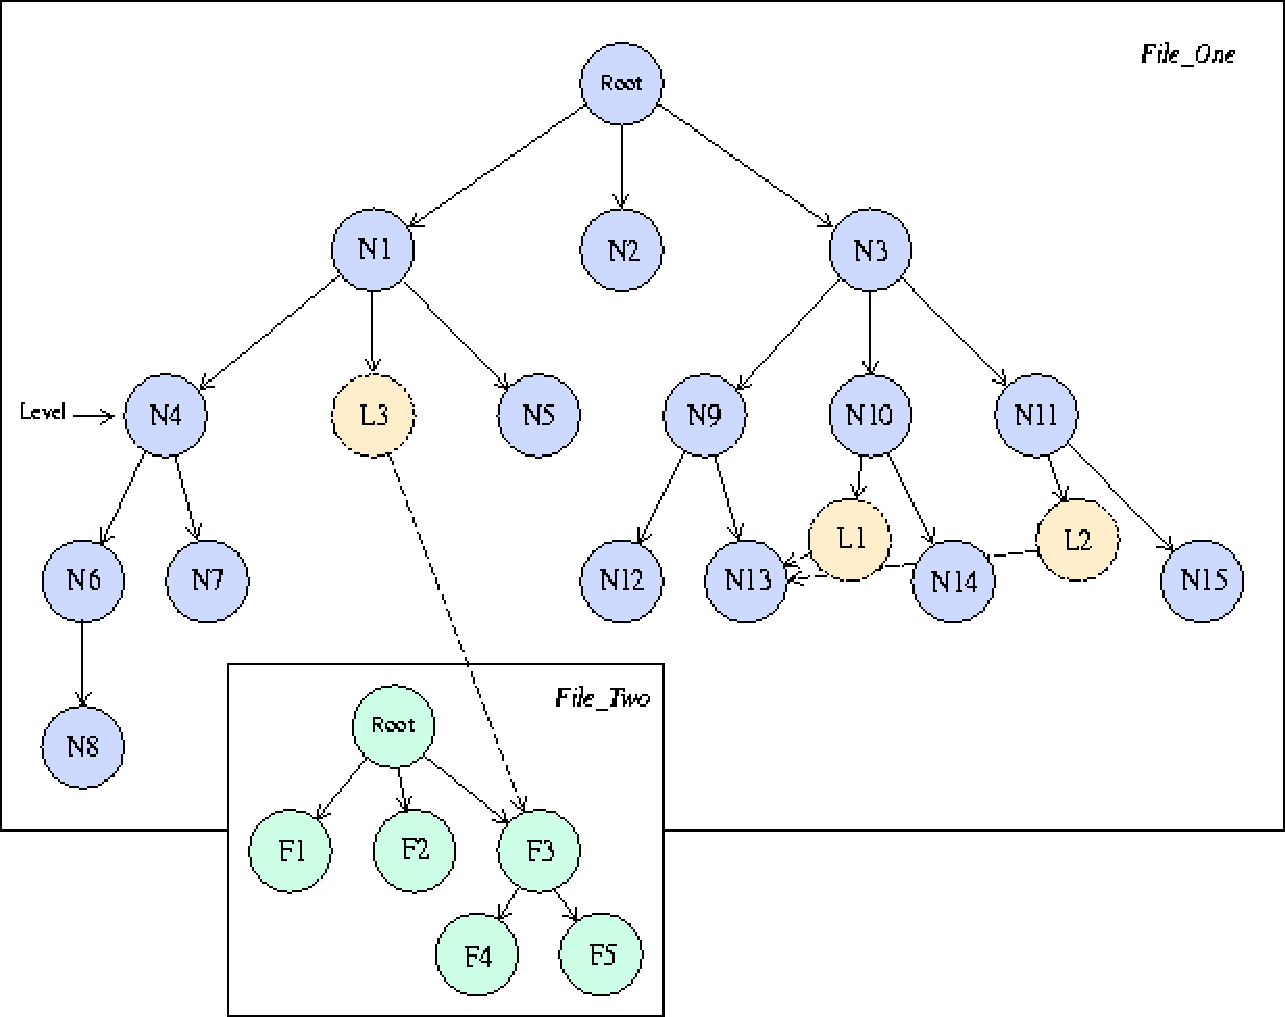
\includegraphics[width=6.0in]{figure}
   \caption{Example Database Hierarchy of Nodes}
   \label{f:example}
\end{figure}

A node knows about itself and its children, but it does not know
anything about its parent.
This means that it is possible to traverse ``down'' the tree by making
queries about what lies below the current node, but it is not possible
to traverse ``up'' the tree by making queries about nodes above a given
node.
If it is desired to move back up the tree, the user must keep track of
that information.

All database files start with a root node, which is created automatically
when a new file is opened.
There is only one root node in a database file, and may be referenced
by the database Root ID or by name as ``\key{/}''.

\subsection{Node Attributes}
\label{s:attributes}

Each node in the database may have zero to many subnodes that are
associated with it, as well as its own data.
The following are a list of attributes accessible by the user for a node
in the hierarchical database system.

\begin{Ventryi}{Number of Dimensions}
\item [Data]
      The data associated with a node.
\item [Data Type]
      A 2-byte character field, blank filled, case sensitive.
      Specifies the type of data (e.g., real, integer, character)
      associated with this node.
      The supported data types are listed in \autoref{t:datatype}
      on p.~\pageref*{t:datatype}.
\item [Dimensions]
      An integer vector containing the number of elements within
      each dimension.
      For example, if the array \fort{A} was declared (using Fortran) as
      \fort{A(10,20)}, the Dimension vector would contain two entries
      (10,20).
\item [ID]
      A unique identifier to access a given node within a file.
      This field contains sufficient information for the database manager
      to locate the node within a file.
      For any given node, the ID is generated only after the file it
      resides in has been opened by a program and the user requests
      information about the node.
      The ID is valid only within the program that opened the file and
      while that file is open.
      If the file is closed and reopened, the ID for any given node
      may be different.
      Within different programs, the node ID for the same node may
      also be different.
      The ID is never actually written into a file.
\item [Label]
      A 32-byte character field.
      The rules for Labels are identical to those for Names.
      Unlike names, Labels do not have to be unique.
      The Label field was introduced to allow ``data typing'' similar to
      the ``typedef'' concept in C.
      Using the Label field in this way allows programs to know some
      additional information about the use of the node itself or its
      child nodes and to call specific subroutines to read the data or
      react in specific ways upon detection of the type.
\item [Name]
      A 32-byte character field.
      The names of child nodes directly attached to a parent node must
      be unique.
      For example, in \autoref{f:example}, all nodes directly attached
      to N3 must have unique names.
      When a request to create a new node is made, the databse manager
      checks the requested name against the other names of the child
      nodes of the specified parent.
      If the requested name is not unique, an error is returned.

      Legal characteristics of a name are a A-Z, a-z, 0-9, and special
      characters (ASCII values from 32 to 126, except for the forward
      slash ``/'' (ASCII number 47)).
      Names will be blank filled to 32 bytes; they are case sensitive.
      Leading blanks are discarded and trailing blanks are ignored,
      whereas internal blanks are significant.

      \emph{Note}: Names passed from C must have the null
      ``\textbackslash0'' character appended to them.
      Names returned through the C interface will have the
      null character appended to them.
      Therefore, C programs should allocate 33 bytes for any Name in
      order to accommodate the null character.

      Fortran programs can allocate 32 characters for Names.
      The Fortran interface takes care of adding or removing the null
      character as required.
\item [Names of Subnodes]
      A list of names of the subnodes (children) of a node.
      (This is the information contained in the child table.)
\item [Number of Dimensions]
      The dimensionality of the data.
      ADF views all data as an array and can handle from zero (i.e., no
      data) to 12 dimensions.
      A ``0'' is used if the data type is empty.
      Thus, a scalar is viewed as a vector with one dimension and
      length 1.
\item [Number of Subnodes]
      The number of child nodes directly attached to any given node.
      Each node can have zero or more child nodes directly associated
      with it.
\item [Pointer]
      An address, from the point of view of a programming language.
      Pointers are like jumps, leading from one part of the data
      structure to another.
\end{Ventryi}

\subsection{Supported Data Types}

\begin{longtable}{l >{\quad}l >{\quad}l >{\quad}l}
\caption[Data Types]{\textbf{Data Types}}
\label{t:datatype}
\\ \hline\hline \\*[-2ex]
\bold{Notation} & \bold{Data Type} & \bold{C Type} & \bold{Fortran Type}
\\*[1ex] \hline\hline \\*[-2ex]
\key{MT} & No Data                 &  & \\
\key{I4} & 32-bit Integer          &  \key{int} & \fort{integer*4} \\
\key{I8} & 64-bit Integer          &  \key{cglong\_t} & \fort{integer*8}\\
\key{U4} & 32-bit Unsigned Integer &  \key{unsigned int} & \fort{integer*4} \\
\key{U8} & 64-bit Unsigned Integer &  \key{cgulong\_t} & \fort{integer*8} \\
\key{R4} & 32-bit Real             &  \key{float} & \fort{real*4} \\
\key{R8} & 64-bit Real             &  \key{double} & \fort{real*8} \\
\key{C1} & Character               &  \key{char} & \fort{character} \\
\key{B1} & Byte (unsigned byte)    &  \key{unsigned char} & \fort{character*1} \\
\key{LK} & Link                    &  &
\\*[1ex] \hline\hline
\end{longtable}

The \key{MT} node contains no data, and is typically used as a
container for subnodes (children).

A link is denoted by \key{LK}, and defines the
linkage between nodes and subnodes. A link provides a mechanism for
referring to a node that physically resides in a different part of the
hierarchy or a different database file. The link parallels a soft link
in the UNIX operating system in that it does not guarantee that the
referenced node exists. The database manager will ``resolve'' the link
only when information is requested about the linked node or it's children.

\subsection{Glossary of Terms}
\label{s:glossary}

\begin{Ventryi}{Node Name}
\item [Child]
      One of the subnodes of a Parent.
      A child node does not have knowledge of its parent node.
      The user must keep track of this relationship.
\item [Database]
      The representation of a hierarchy of nodes on disk files.
      By use of links, it may physically span multiple files.
\item [File]
      An database file, which a single root node and its underlying structure.
\item [ID]
      A unique identifier to access a given node within a database file.
      This field contains sufficient information for the database manager
      to locate the node within a file.
      For any given node, the ID is generated only after the file it
      resides in has been opened by a program and the user requests
      information about the node.
      The ID is valid only within the program that opened the file and
      while that file is open.
      If the file is closed and reopened, the ID for any given node
      may be different. Within different programs, the node-ID for the
      same node may also be different.
      The ID is never actually written into a file.
\item [Link-Node]
      A special type of node.
      Links are created using the
      \hyperlink{create_link}{\key{cgio\_create\_link}}
      subroutine.
      The data type of this node is \key{LK}, and its data is a
      one-dimensional array containing the name of the file (if other
      than the current file) containing the node to be linked and the
      full path name in that file from the root node to the desired
      node.

      Links provide a mechanism for referring to a node that physically
      resides in a different part of the hierarchy.
      The node pointed to by a link may or may not reside in the same
      file as the link itself.
      A link within ADF is very similar to a ``soft'' link in the
      UNIX operating system in that it does not guarantee that the
      referenced node exists.
      ADF will ``resolve'' the link only when information is requested
      about the node.
      If the ID of a link-node is used in an ADF call, the effect of
      the call is the same as if the ID of the linked-to node was used.
      Note that a link node does not have children itself.
      In \autoref{f:example} on p.~\pageref*{f:example}, the children
      seen for \key{L3} are \key{F4} and \key{F5}.
      If a child is ``added'' to \key{L3}, then in reality, the child
      is added to \key{F3}.
      There are specialized subroutines provided to create link nodes
      and extract the link details.
\item [Node]
      The single component used to construct a database.
\item [Node name]
      A node has a 32-character name.
      Every child node directly under a given parent must have a unique
      name.
      Legal characteristics in a name are \key{A-Z}, \key{a-z},
      \key{0-9}, and special characters (ASCII values from 32 to
      126, omitting the forward slash ``\key{/}'', ASCII number 47).
      Names will be blank filled to 32 bytes; they are case sensitive.
      Leading blanks are discarded and trailing blanks are ignored,
      whereas internal blanks are significant.
\item [Parent]
      A node that has subnodes directly associated with it.
\item [Pathname]
      Within a database, nodes can be referenced using the name of a node
      along with its parent ID, or by using a ``pathname'' whose syntax is
      roughly the same as a path name in the UNIX environment.
      A pathname that begins with a leading slash ``\key{/}'' is
      assumed to begin at the root node of the file.
      If no leading slash is given, the name is assumed to begin at the
      node specified by the parent ID.
      Although there is a 32-character limitation on the node Name,
      there is no restriction on the length of the pathname.
      For example, equivalent ways to refer to node \key{N8} in
      \autoref{f:example} are:
      \begin{itemize}
      \item Node-ID for \key{N6} and name = ``\key{N8}''
      \item Node-ID for \key{N4} and name = ``\key{N6/N8}''
      \item Node-ID for \key{N1} and name = ``\key{N4/N6/N8}''
      \item Node-ID for the \key{Root\_Node} and name =
            ``\key{/N1/N4/N6/N8}''
      \end{itemize}
\end{Ventryi}

\subsection{Conventions and Implementations}
\label{s:conventions}

\begin{Ventryi}{return codes}
\item [C]
      All input strings are to be null terminated.
      All returned strings will have the trailing blanks removed and
      will be null terminated.
      Variables declared to hold Names, Labels, and Data-Types should
      be at least 33 characters long.
      \textit{cgns\_io.h} has a number of variables defined.
      An example declaration would be:
\begin{indlefttt}
char name[CGIO\_MAX\_NAME\_LENGTH+1];
\end{indlefttt}
\item [Fortran]
      Strings will be determined using inherited length.
      Returned strings will be blank filled to the specified length.
      All returned names will be left justified and blank filled on the
      right.
      There will be no null character.
      An example declaration would be:
\begin{indlefttt}
PARAMETER CGIO\_MAX\_NAME\_LENGTH=32
CHARACTER*(CGIO\_MAX\_NAME\_LENGTH) NAME
\end{indlefttt}
      or include the Fortran header file \textit{cgns\_io\_f.h}
      which defines these parameters.
\item [ID]
      A unique identifier to access a given node within a database.
      For any given node, the ID is generated only after the file it
      resides in has been opened by a program and the user requests
      information about the node.
      The ID is valid only within the program that opened the file and
      while that file is open.
      If the file is closed and reopened, the ID for any given node
      may be different.
      Within different programs, the node ID for the same node may
      also be different.
      The ID is not ever actually written into a file.

      The declaration for variables that will hold node IDs should be
      for an 8-byte real number.
\item [Indexing]
      All indexing is Fortran-like in that the starting index is 1 and
      the last is \fort{N} for $N$ items in an index or array
      dimension.
      The array structure is assumed to be the same as in Fortran
      with the first array dimension varying the fastest and the last
      dimension varying the slowest.
 
      The index starting at one is used in
      \hyperlink{read_data}{\key{cgio\_read\_data}},
      \hyperlink{write_data}{\key{cgio\_write\_data}},
      \hyperlink{children_names}{\key{cgio\_children\_names}}, and
      \hyperlink{children_ids}{\key{cgio\_children\_ids}}.
 
      The user should be aware of the differences in array indexing
      between Fortran and C.
      The subroutines
      \hyperlink{read_all_data}{\key{cgio\_read\_all\_data}} and
      \hyperlink{write_all_data}{\key{cgio\_write\_all\_data}}
      merely take a pointer to the beginning of the data, compute how
      much data is to be read/written, and process as many bytes as
      have been requested.
      Thus, these routines effectively make a copy of memory onto disk
      or vice versa.
      Given this convention, it is possible for a C program to
      use standard C conventions for array indexing and use
      \key{cgio\_write\_all\_data} to store the array on disk.
      Then a Fortran program might use \key{cgio\_read\_all\_data} to
      read the data set.
      Unless the user is aware of the structure of the data, it is
      possible for the array to be transposed relative to what is
      expected.
 
      The implications of the assumed array structure convention can be
      quite subtle.
      The subroutines \key{cgio\_write\_data} and
      \key{cgio\_read\_data} assume the Fortran array structure in
      order to index the data.
      Again, unless the user is aware of the implications of this, it
      is possible to write an array on disk and later try to change a
      portion of the data and not change the correct numbers.
 
      As long as users are aware of how their data structure maps onto
      the database, there will not be any problems.
\item [return codes]
      The CGIO routines return an integer code indicating whether they
      were successfull or not. On success, 0 (\key{CGIO\_ERR\_NONE}) is
      returned. A non-zero return indicates an error. Return codes < 0
      indicate an error at the CGIO level; codes > 0 indicate an
      error in the database manager. See
      \hyperlink{s:messages}{Error Messages} for a list of
       error codes and mesages.
\end{Ventryi}

\subsection{Limits and Sizes}
\label{s:defaults}

The following default values, sizes, and limits are defined in the
header file \textit{cgns\_io.h}.

\begin{longtable}{l >{\quad}l >{\quad}l}
\caption[Default Values and Sizes]{\textbf{Default Values and Sizes}}
\label{t:defaults}
\\ \hline\hline \\*[-2ex]
\bold{Define} & \bold{Value} & \bold{Attribute}
\\*[1ex] \hline\hline \\*[-2ex]
\key{CGIO\_MAX\_DATATYPE\_LENGTH} & 2    & Data type length \\
\key{CGIO\_MAX\_DIMENSIONS}       & 12   & Maximum dimensions \\
\key{CGIO\_MAX\_NAME\_LENGTH}     & 32   & Name length \\
\key{CGIO\_MAX\_LABEL\_LENGTH}    & 32   & Label length \\
\key{CGIO\_MAX\_VERSION\_LENGTH}  & 32   & Version length \\
\key{CGIO\_MAX\_DATE\_LENGTH}     & 32   & Date length \\
\key{CGIO\_MAX\_ERROR\_LENGTH}    & 80   & Maximum length of error string \\
\key{CGIO\_MAX\_LINK\_DEPTH}      & 100  & Maximum link depth \\
\key{CGIO\_MAX\_FILE\_LENGTH}     & 1024 & File name length \\
\key{CGIO\_MAX\_LINK\_LENGTH}     & 4096 & Maximum link data size
\\*[1ex] \hline\hline\hline
\end{longtable}



\clearemptydoublepage
\appendix
\section{ADF Glossary of Terms}
\label{s:glossary}
\thispagestyle{plain}

\begin{Ventryi}{Node Name}
\item [ADF]
      The initialism (acronym) for Advanced Data Format.
\item [Child]
      One of the subnodes of a Parent.
      A child node does not have knowledge of its parent node.
      The user must keep track of this relationship.
\item [Database]
      A hierarchy of ADF nodes.
      By use of links, it may physically span multiple files.
\item [File]
      An ADF file, which a single root node and its underlying structure.
\item [ID]
      A unique identifier to access a given node within a file.
      This 8-byte field contains sufficient information for ADF to
      locate the node within a file.
      For any given node, the ID is generated only after the file it
      resides in has been opened by a program and the user requests
      information about the node.
      The ID is valid only within the program that opened the file and
      while that file is open.
      If the file is closed and reopened, the ID for any given node
      will be different.
      Within different programs, the node-ID for the same node will be
      different.
      The ID is never actually written into a file.
\item [Link-Node]
      A special type of node.
      Links are created using the \hyperlink{sub:Link}{\fort{ADF\_Link}}
      subroutine.
      The data type of this node is \fort{LK}, and its data is a
      one-dimensional array containing the name of the file (if other
      than the current file) containing the node to be linked and the
      full path name in that file from the root node to the desired
      node.

      Links provide a mechanism for referring to a node that physically
      resides in a different part of the hierarchy.
      The node pointed to by a link may or may not reside in the same
      file as the link itself.
      A link within ADF is very similar to a ``soft'' link in the
      UNIX operating system in that it does not guarantee that the
      referenced node exists.
      ADF will ``resolve'' the link only when information is requested
      about the node.
      If the ID of a link-node is used in an ADF call, the effect of
      the call is the same as if the ID of the linked-to node was used.
      Note that a link node does not have children itself.
      In \autoref{f:example} on p.~\pageref*{f:example}, the children
      seen for \fort{L3} are \fort{F4} and \fort{F5}.
      If a child is ``added'' to \fort{L3}, then in reality, the child
      is added to \fort{F3}.
      There are specialized subroutines provided to create link nodes
      and extract the link details.
\item [Node]
      The single component used to construct an ADF database.
\item [Node name]
      A node has a 32-character name.
      Every child node directly under a given parent must have a unique
      name.
      Legal characteristics in a name are \fort{A-Z}, \fort{a-z},
      \fort{0-9}, and special characters (ASCII values from 32 to
      126, omitting the forward slash ``\fort{/}'', ASCII number 47).
      Names will be blank filled to 32 bytes; they are case sensitive.
      Leading blanks are discarded and trailing blanks are ignored,
      whereas internal blanks are significant.
\item [Parent]
      A node that has subnodes directly associated with it.
\item [Pathname]
      Within a database, nodes can be referenced using the name of a node
      along with its parent ID, or by using a ``pathname'' whose syntax is
      roughly the same as a path name in the UNIX environment.
      A pathname that begins with a leading slash ``\fort{/}'' is
      assumed to begin at the root node of the file.
      If no leading slash is given, the name is assumed to begin at the
      node specified by the parent ID.
      Although there is a 32-character limitation on the node Name,
      there is no restriction on the length of the pathname.
      For example, equivalent ways to refer to node \fort{N8} in
      \autoref{f:example} are:
      \begin{itemize}
      \item Node-ID for \fort{N6} and name = ``\fort{N8}''
      \item Node-ID for \fort{N4} and name = ``\fort{N6/N8}''
      \item Node-ID for \fort{N1} and name = ``\fort{N4/N6/N8}''
      \item Node-ID for the \fort{Root\_Node} and name =
            ``\fort{/N1/N4/N6/N8}''
      \end{itemize}
\end{Ventryi}


\clearemptydoublepage
\section{History and Current Status}
\label{s:history}
\thispagestyle{plain}

\subsection{Initial Development}

\enlargethispage{\baselineskip}
The initial development of CGNS took place from March 1995 through
May 1998, when Version 1.0 of the CGNS software was released.
The project originated through a series of meetings in 1994-1995 between
NASA, Boeing, and McDonnell Douglas, who were then working under the
Integrated Wing Design element of NASA's Advanced Subsonic Technology
Program.
The work being planned involved extensive use of CFD, and the
possibility of collaborative analyses by many organizations.
It was thus necessary to establish a common data format suitable to meet
the needs of production CFD tools in the mid- to late-1990s.
This format would be used to enable interchange of data among different
CFD-related tools and different computing platforms, and to provide a
mechanism for archive and retrieval of CFD data

At that time, the \textit{de facto} standard for CFD data was the file
format used by Plot3D, a flow visualization program developed at NASA
Ames.
However, the Plot3D format was developed to expedite post-processing,
and was never intended as a general-purpose standard for the storage
and exchange of CFD data.
By the early 1990s, as CFD became more sophisticated, the limitations of
the Plot3D format as a general-purpose standard had become apparent.
It had no provisions for storing data associated with modern CFD
technology, such as unstructured grids, turbulence models based on
solutions of partial differential equations, and flows with multiple
chemical species.

Individual organizations were overcoming these limitations by defining
extensions to the Plot3D format to meet their needs.
These extensions were not coordinated among different organizations, and
therefore data stored in these extended formats generally could not be
utilized outside the originating organization.
Further, the Plot3D format was not self-documenting, and it was
necessary to rely on file-naming conventions or external notes to
maintain awareness of the flow conditions and analyzed geometry of each
PLOT3D data file.

To overcome these limitations, several database options were considered
by the NASA~/ Boeing~/ McDonnell Douglas team from December 1994 to
March 1995.
In March 1995, the decision was made to build a new data standard called
CGNS (Complex Geometry Navier Stokes).
This standard was a ``clean sheet'' development, but it was heavily
influenced by the McDonnell Douglas Common File Format (CFF), which had
been established and deployed in 1989 and heavily revised in 1992.

Agreement was reached to develop CGNS at Boeing, under NASA Contract
NAS1-20267, with active participation by a team of CFD researchers from

\begin{itemize*}
   \item NASA Langley Research Center
   \item NASA Glenn Research Center
   \item NASA Ames Research Center
   \item McDonnell Douglas Corporation (now Boeing St. Louis)
   \item Boeing Commercial Airplane Group (Seattle) Aerodynamics
   \item Boeing Commercial Airplane Group (Seattle) Propulsion
   \item ICEM CFD Engineering Corporation
\end{itemize*}

The original development work itself occurred from 1995--1998, and
consisted of essentially four activities:

\begin{itemize*}
\item Development of the standalone database manager (the ADF Core)
\item Identification and layout of the CFD data (the SIDS and File
      Mapping)
\item Development of an API for use in applications codes (the
      Mid-Level Library)
\item Demonstration of system capability
\end{itemize*}

\subsubsection{Development of ADF}

As noted earlier, the decision to develop CGNS was made after an
examination of several existing formats.
Because of its hierarchical structure, the CFF (Common File Format) that
was then in use at McDonnell Douglas was judged the most compatible with
the SIDS.
However, CFF had known limitations, and it was decided to adopt the CFF
structure but recast it in a more general form.
This gave the developers control over the software and facilitated the
development of a robust, portable, reliable, and flexible database
manager, which could be distributed freely within the system.

These low-level routines were developed during 1995, and make up the
ADF (Advanced Data Format) Core.
ADF was written and extensively tested at Boeing by a small subteam
familiar with standard software development practices, and it may now be
considered a stable product.

\subsubsection{Identification and layout of the CFD data}

Another task, undertaken in parallel with the development of ADF, was to
identify the data associated with CFD and establish a means of encoding
it within the ADF format.
This task was the primary concern of the national team, with Boeing
proposing the standards and the remainder of the team serving to
critique, test, and improve them.
This began with the development of the SIDS and its language.
The hierarchical nature of the SIDS was used to suggest the SIDS-to-ADF
File Mapping conventions, which were developed slightly after the SIDS
but along the same track.

\subsubsection{Development of an API}

At a review in June 1997, the CGNS team (NASA, Boeing, and McDonnell
Douglas) determined that additional support would be required to produce
an adequate Mid-Level Library.
Subcontracts were issued to the ICEM CFD Engineering Company, in
Berkeley, CA, following this decision.
ICEM CFD in effect became the lead organization for the development of
the Mid-Level Library.

Also at this time, the acronym ``CGNS'' was re-defined to mean ``CFD
Generalized Notation System'', which was more in keeping with the evolved
goals of this project.

Version 1.0 of the Mid-Level Library, which met the original goal of
supporting structured multi-block analysis codes, was released in May
1998.
This set of higher-level routines enables a user to implement the CFD
standards defined by the SIDS, without specific knowledge of the File
Mapping or the ADF Core.
This activity was crucial to the acceptance and implementation of CGNS
among the CFD community.

NASA and the informal CGNS committee determined that there was no
need for export authority so the CGNS standard, the ADF Core and the
Mid-Level Library, and all supporting documentation could be distributed
worldwide as freeware.
Appropriate legal reviews and approvals were obtained at both NASA and
Boeing to validate this decision.

\subsubsection{Demonstration of system capability}

\paragraph{Prototypes.}
To test the CGNS data recording and retrieval mechanisms and to
gain experience with the installation of the software into common
applications codes, the developers modified two CFD solvers (namely,
NPARC and TLNS3D) to operate in the CGNS environment.
In addition, NASA Langley Research Center modified CFL3D similarly.
These modifications were made early in the project and predate the
Mid-Level Library and some later portions of the SIDS.

Separate data cases were prepared for each of the prototypes.
Each prototype proved capable of starting, exiting, and restarting its
data case as expected.
In addition, in all three cases, transfer of the CGNS data between
workstation (SGI) and mainframe (CRAY) platforms was successfully
demonstrated.

Dissimilarity of the \emph{content} of the data required by NPARC
and the other two codes (i.e., nodal vs. cell-centered data) prevented
restarting NPARC from TLNS3D/CFL3D data and vice versa.
However, this type of restart was demonstrated between TLNS3D and CFL3D.

These prototypes were limited in certain ways and, therefore, were not
suitable as a final implementation of their respective capabilities in
CGNS.
The principal limitations are:

\begin{itemize}
\item The prototypes implement only the grid coordinates, flow solution,
      boundary condition, and 1-to-1 interface connectivity portions of
      the CGNS data specification.
\item No attempt was made to modify the internal structure of any of
      the codes in order to improve compatibility with CGNS data
      organization.
\item The prototypes accessed the ADF files primarily using routines
      at the ADF Core level.
      There were some higher-level routines included, and these, in many
      cases, suggested the content of the CGNS Mid-Level Libraries.
      But the high-level prototype routines often intermingled
      ADF functions with CGNS functions and, in some cases, were
      code-specific or dependent on internal directives to make them so.
      They were thus less broadly applicable than the current Mid-Level
      Library routines.
\item These codes exercised only a portion of the CGNS boundary
      condition specifications. 
\item The prototypes sometimes incorporated extra nodes into their ADF
      files to carry code-specific data.
      This practice arose partially from the lack of complete CGNS data
      specifications at the time the prototypes were written, but it
      resulted also, in part, because the current code input structure
      required a different (but equivalent) form of the CGNS data, and
      the developers opted to duplicate it within the CGNS database.
\end{itemize}

The general lesson learned from the construction of the prototypes
was that professional programmers had no conceptual difficulty in
implementing CGNS at the ADF Core level.
But the resulting code was cumbersome, and the development of the
Mid-Level Library was needed to facilitate dissemination of CGNS among
those disinclined to work with the ADF Core.

\paragraph{System Demonstrator.}
As the CGNS effort progressed, an additional activity was undertaken
to demonstrate the capability of the mature system.
Known as the ``system demonstrator'', this tested the ability of CGNS to
transfer data seamlessly between applications that had never operated
together before.
The system demonstrator used most of that portion of the currently
existing SIDS that has been included in the Mid-Level Library.

The geometry chosen for the test was a high-lift configuration known as
the trapezoidal wing.
This is a multielement airfoil with a full-span slat and flap, and a
generic fuselage.

Three separate CGNS-compatible application codes were involved in the
system demonstrator.

\begin{Ventryic}{OVERFLOW}
\item [GMAN]
      A pre-processor and grid generation tool developed by Boeing
      St. Louis
\item [OVERFLOW]
      A CFD flow solver developed by NASA Ames
\item [Visual3]
      A flow visualization tool from ICEM CFD, originally developed at
      MIT
\end{Ventryic}

The system demonstrator consisted of the following tasks:

\begin{enumerate}
\item The grid was generated using NASA Ames grid tools and written
      as a Plot3D file.
\item The grid file was sent to Boeing St. Louis, where it was processed
      by a locally-modified version of GMAN.
      GMAN calculated the grid connectivity information, and wrote the
      grid and connectivity data into a CGNS database.
      Boundary conditions were also added to the CGNS database at this
      time.
\item The CGNS file was returned to NASA Ames, where it was read by the
      newly-modified OVERFLOW code.
      (Some iteration was necessary here, because the definition of
      overset holes used by GMAN differs from that normally expected by
      OVERFLOW.
      The CGNS file was intact, and served, as intended, to highlight the
      discrepancy.)
      OVERFLOW computed the flow field, writing the results into the
      CGNS database.
\item The CGNS file was next sent to ICEM CFD.
      There, the CGNS database was read and displayed using Visual3.
\end{enumerate}

The system demonstrator involved significant cross-platform transfer
among various workstation and mainframe computing facilities.
The results indicated that universal data exchange was well supported by
CGNS.

\subsection{Subsequent Development}

\subsubsection{Software}

Since the release of Version 1.0 of the CGNS software in May 1998,
several improvements and extensions have been made to the SIDS, the File
Mapping, and the Mid-Level Library.

\begin{itemize}
\item Version 1.1, released in June 1999, added support for
      unstructured grids, and for associating CAD geometric entities
      with grid surfaces.
\item Version 2.0, released in December 2000, added support for
      moving and/or deforming grids, and for iterative/time-dependent
      data.
\item Version 2.1, released in May 2002, added support for
      user-defined data arrays, chemistry, and linked nodes.
\item Version 2.2, released in May 2003, added support for axisymmetry
      information, rotating coordinates, special properties associated
      with particular grid connectivity patches, such as periodicity or
      averaging, special properties associated with particular boundary
      condition patches, such as wall functions and bleed, and gravity.
\item Version 2.3, released in Jan 2004, restored the capability to
      specify a boundary condition patch using \fort{ElementRange} or
      \fort{ElementList}.
\item Version 2.4, released in Aug 2005, added support for describing
      electric field, magnetic field, and conductivity models used
      in electromagnetic flows, specification of units for electric
      current, substance amount, and luminous intensity, more flexible
      specification of boundary condition locations, and additional
      user-defined data.
      Also new in Version 2.4 is the ability to choose, at build time,
      either ADF or HDF5 as the underlying database manager.
\item Version 2.5, released in Sep 2007, added Mid-Level Library
      functions to check file validity, configure some internal CGNS
      library options, and provide alternate ways to access a node.
      Some changes were also made in the use of functions for partial
      writes of coordinate, element, and solution data.
      Support was also added for building the CGNS library as a DLL under
      Windows.
\end{itemize}
A more detailed list of revisions to the CGNS software is available at
the CGNS web site.

ICEM CFD served as the focal point for CGNS software development through
the release of Version 2.0, plus the changes in Version 2.5, using
internal company resources.
New features in Version 2.1 and 2.4 were added by Intelligent Light,
with funding from NASA Langley.
Eagle Aeronautics, with additional participation by ICEM CFD, added the
new features in Version 2.2, again with funding from NASA Langley.
Support for HDF as the underlying database in Version 2.4 was added
by personnel from ONERA, ICEM CFD, and the U. S. Air Force Arnold
Engineering Development Center.

\subsubsection{Management and Support}

In 1998 NASA announced that the Advanced Subsonic Technology program,
which had funded the initial CGNS development, would end in September
1999.
Several organizations interested in the continued development of CGNS
met in May 1999 to discuss options.
The decision was made to create the CGNS Steering Committee, a voluntary
public forum made up of international representatives from government
and private industry.

The Steering Committee is responsible for coordinating the further
development and dissemination of the CGNS standard and its supporting
software and documentation.
In Jan 2000, the CGNS Steering Committee became a Sub-committee of the
AIAA CFD Committee on Standards.
Additional details about the mission and responsibilities of the
Steering Committee, and its organization, are in the \textit{CGNS Steering
Committee Charter}.

The basic CGNS documentation has of course been updated to reflect the
software changes described above.
In addition, all the documentation has been converted to LaTeX (used
to create PDF versions for printing), and to HTML (for interactive
use).
A new document, \textit{A User's Guide to CGNS}, was made available in
October 2001, and is very useful for new and prospective users of the
Mid-Level Library.

To encourage communication between CGNS users, a mailing list called
CGNStalk was created in Oct 2000.
Instructions for subscribing are available at the CGNS web site.

\subsection{Current Status}

Since the initial release of the Mid-Level Library in May 1998,
interest in CGNS has continued to grow throughout the global CFD
community.
The system is being used by engineers and scientists in academia,
industry, and government.
By January 2002, 591 users from more than 25 countries had formally
registered at the CGNS web site.
As of September 2007, the CGNStalk mailing list had 224 participants
from 20 different countries and at least 79 different organizations.

\subsubsection{Software}

The current ``production'' release of CGNS is Version 2.5, released in
September 2007.

Several extensions to CGNS have been formally proposed.
Documentation supporting these extensions, and information on their
current status, is available via the ``Proposals for Extensions'' link at
the CGNS web site.

\subsubsection{Standards}

Between 1999 and 2002, an effort was spearheaded by Boeing to establish
an ISO-STEP standard for the representation, storage, and exchange of
digital data in fluid dynamics based on the CGNS standard.
Unfortunately, the effort had to be curtailed because of budget
problems.
It was subsequently decided that an existing ISO standard on finite
element solid mechanics would be rewritten and submitted to include CGNS
as well as an integrated engineering analysis framework.

As part of its role as a sub-committee of the AIAA CFD Committee
on Standards, the CGNS Steering Committee is also involved in the
development of the AIAA Recommended Practice for the storage of CFD
data.
The Recommended Practice consists of the CGNS Standard Interface
Data Structures (SIDS) document, reformatted to conform to AIAA's
requirements.
The current AIAA Recommended Practice (corresponding to CGNS Version
2.4) is available at the
\href{http://www.aiaa.org/content.cfm?pageid=363&id=1657}{AIAA
Online Store}, and as a
\href{http://www.grc.nasa.gov/www/cgns/sids/aiaa/R_101A_2005.pdf}{PDF file}
(1.01M, 200 pages) at the CGNS Documentation web site.

\subsection{Noteworthy Contributions}

The entire CGNS team deserves credit for its accomplishments.
The project might easily be cited as a prime example of effective
voluntary cooperation between government and industry.
Every member has contributed ideas, enthusiasm, and improvements, and
enabled us to represent a cross-section of knowledge and practice from
the CFD community.

It would not be practical to outline each member's contributions to a
project of this complexity.
Nevertheless, it is appropriate to note the contributions of a few
individuals who dedicated special effort during the crucial stages
leading to the initial release of CGNS in May 1998.

\begin{itemize}
\item Steve Allmaras conceived, pursued, and completed the SIDS and
      developed the language in which it is written.
\item Tom Dickens, Matt Smith, and Wayne Jones designed the ADF Core.
\item Tom Dickens wrote the ADF Core.
\item Dan Owen maintained and tuned the ADF Core after Tom left the group.
\item Chuck Keagle designed and executed stringent testing procedures
      for the ADF Core; that is to say, he did everything he could think
      of to break it.
\item Diane Poirier designed and wrote the CGNS Midlevel Library and
      drafted the original proposals for unstructured grid.
      She and Alan Magnuson drafted the proposals for CAD-to-geometry
      specifications.
\item Gary Shurtleff wrote the TLNS3D and NPARC prototypes and provided
      us with what was, for a long time, the only examples of working
      CGNS software.
\item Chris Rumsey served as liaison with NASA Langley, responding in
      detail to requests for criticism and improvements and testing the
      system by writing the CFL3D prototype.
\item Cetin Kiris converted the OVERFLOW code to CGNS, twice.
\item Wayne Jones tested our abstractions with real code, which found
      its way into the ADF Midlevel Library and the CGNS Toolkit.
\item Matt Smith wrote much of the File Mapping and ADF Core documents
      and, with knowledge of both CFD and software design, brought good
      sense to bear on proposals that needed it.
\item Ray Cosner's retrospective vantage point made him a reliable
      supporter who was often able to move things forward when progress
      slowed.
\item Susan Jacob supplied initial guidance as a Productivity+ coach and
      got us all moving in (more or less) the same direction.
\item Doug McCarthy led the project to completion.
\item Shay Gould made the documentation intelligible and presentable.
\end{itemize}

\noindent
And, a particularly special mention:

\begin{itemize}
\item Ben Paul secured the initial funding and shepherded the project
      through the early phases of the contract.
      We will never forget the many meetings Ben held to make sure that
      he thought that he knew that we thought that we knew what we needed
      to do, and that we were doing it.
      His patience and good-natured perseverance could not have been
      replaced.
\end{itemize}


\clearemptydoublepage
\section{ADF File System Architectures}
\label{s:arch}
\thispagestyle{plain}

The following platform architectures have been tested and used both for
functionality testing of the ADF core software libraries and for testing
and running the prototype.

\begin{longtable}{l >{\quad}l >{\quad}l >{\quad}l}
\caption[Platform Architectures]{\textbf{Platform Architectures}}
\label{t:arch}
\\ \hline\hline \\*[-2ex]
\bold{Release} & \bold{Machine} & \bold{OS Version} & \bold{Native Format}
\\*[1ex] \hline\hline \\*[-2ex]
A01 & Cray          & Unicos 8.0  & Unicos 8.0 \\
A01 & SGI/IRIS      & 4.0.5       & IEEE Big Endian\footnote{
   In the table, ``Endian'' refers to the ordering of bytes in a
   multi-byte number.
   Big endian is a computer architecture in which, within a given
   multi-byte numeric representation, the most significant byte has the
   lowest address (the word is stored ``big-end-first'').
   Little endian is a computer architecture in which, within a given 16-
   or 32-bit word, bytes at lower addresses have lower significance (the
   word is stored ``little-end-first'').} \\
B01 & HP            & 9.05        & IEEE Big Endian \\
B01 & SGI/IRIS      & 5.03        & IEEE Little Endian \\
C00 & Intel Paragon & ---         & IEEE Little Endian \\
C00 & Dec Alpha     & ---         & IEEE Little Endian \\
C00 & SGI/IRIS      & 6.2         & IEEE Big Endian \\
C00 & Cray T90      & Unicos 9.02 & Cray Format
\\*[1ex] \hline\hline
\end{longtable}


\clearemptydoublepage
\section{ADF File Version Control Numbering}
\label{s:versions}
\thispagestyle{plain}

The ADF file version control number scheme is described below.
The format for the version number is a field of six digits or characters:
\begin{indlefttt}
AXXxxx
\end{indlefttt}
where:

\begin{Ventryi}{\fort{xxx}}
\item [\fort{A}]
      Major revision number.
      Major internal structure changes.
      This number is not expected to change very often, if at all,
      because the backward compatibility is only available by explicit
      policy decision.

      One alphabetic character.

      Range of values: \fort{A-Z}, \fort{a-z}

      In the unlikely event of reaching \fort{z}, then use any other
      unused printable ASCII character, except the blank or symbols
      used by the ``\textit{what}'' command 
\begin{indlefttt}
@()#~>\textbackslash
\end{indlefttt}
\item [\fort{XX}]
      Minor revision number.
      New features, minor changes, and bug fixes.
      Backward but not forward compatible.

      Two-digit hexadecimal number (uppercase letters).

      Range of values: \fort{00-FF}

      Reset to \fort{00} with changes in major revision number.
\item [\fort{xxx}]
      Incremental number.
      Incremented with every new version of the library (even if no
      changes are made to the file format).
      Files are forward and backward compatible.

      Three-digit hexadecimal number (lowercase letters).

      Range of values: \fort{000-fff}

      Does not reset.
\end{Ventryi}

\noindent
The following definitions are used:

\begin{Ventryi}{Backward compatible}
\item [Forward compatible]
      Older versions of libraries can read and write to files created
      by newer versions of libraries.
\item [Backward compatible]
      Newer versions of libraries can read and write to files created
      by older versions of libraries.
\end{Ventryi}



\clearemptydoublepage
\section{ADF Design Considerations}
\label{s:design}
\thispagestyle{plain}

This section provides a summary of the design considerations that were
used in the construction of the ADF software library.

\subsection{ADF File Header Information}

Every ADF file has a header section that contains information about the
file itself.
The following information from this header is available to the user:

\begin{itemize}
\item ADF version number of the library that created the database.
\item File creation date and time.
\item File modification date and time.
\item Data format used in database (IEEE big endian, IEEE little endian,
      etc.)
\end{itemize}

[Under data format, ``endian'' refers to the ordering of bytes in a
multi-byte number.
Big endian is a computer architecture in which, within a given
multi-byte numeric representation, the most significant byte has the
lowest address (the word is stored ``big-end-first'').
Little endian is a computer architecture in which, within a given 16- or
32-bit word, bytes at lower addresses have lower significance (the word
is stored ``little-end-first'').]

\subsection{ADF File Optimizations}

To optimize the performance of ADF, the following techniques have been
incorporated into the ADF software to enhance performance of the file:

\begin{itemize}
\item Use block-based, unbuffered (raw mode) I/O where available, with
      block sizes of 4096 bytes.
\item Align medium to large data chunks on block boundaries.
\item If the data size is equal to or greater than 2048, then
      \begin{itemize}
      \item align data to the next block and
      \item add extra to free (garbage) lists
      \end{itemize}
\item Avoid, where possible, small- to medium-sized chunks of data that
      span block boundaries.
\item Align, where possible, to the next block and add extra to free
      (garbage) lists.
\end{itemize}

Allow data space to grow by linking data chunks.
It is possible to increase the last dimension; doing so will extend the
data.
However, internal dimensional changes will corrupt the existing data.

The pointer table for child nodes will also contain the child node names.

\subsection{ADF File Portability}

To address code portability and future needs, the following design
decisions were made:

\begin{itemize}
\item Use larger than 32-bit file pointers to allow for files larger than
      4 Gigabytes.
      (C routine \fort{lseek} may not handle this, but ADF files should
      allow it.)
\item Use 48-bit pointers within a block of data.
      32-bit pointers to 4096-byte blocks and a 16-bit pointer to a
      position within the block.
      This allows for files with 4 gigabyte blocks, in other words
      $2^{32} \times 4096 = 17.5922 + 12$ bytes or 17.59 Tera bytes.
\item The ID pointers will be 64-bit coded IDs.
      Users may use double data type (\fort{real*8}).
      This is parceled as follows: 32 bits for block number, 12 bits for
      block offset, and 20 bits for file identifier.
\item Encode the integer information, other than data, in ASCII,
      Hex-based notation.
\end{itemize}

\subsection{ADF File Error Checking}

Error checking has been implemented for the ADF file and is summarized
here.
Each item in the ADF file will have item-specific boundary tags
surrounding it to provide file-based corruption checking.
For variable-sized items, the associated boundary tags will include
file-based size information.
Information will be written to the disk in a sequence that will not
allow corrupt files.
For example, when adding a new child node, the complete child
information will be written before the parent's child-table is updated.
An ADF-core subroutine for downloading data to disk will be provided.

\subsection{ADF Source Code Considerations}

The ADF library of source code will incorporate the use of UNIX ``what''
strings for the ADF version number and also RCS versioning information
in the source code and in the object code.
The source code is written in portable ANSI C, using POSIX-defined system
calls.

\subsection{ADF Node Header Information}

The following information is contained in an ADF node header:

\begin{itemize}
\item node boundary tag
\item name (32 characters)
\item label (32 characters)
      \begin{itemize}
      \item number of subnodes (\fort{num\_sub\_nodes}) is an integer
            (ASCII, Hex encoded in file).
      \item address pointer of the subnodes indicated by the variable.
      \end{itemize}
\item \fort{sub\_nodes}, which are pointers (ASCII, Hex encoded in file)
      to a table (the ``child table'') of file pointers and names for each
      of the node's children.
      Note that the child name information is redundant and included for
      performance.
\item data type is specified in \fort{data\_type} (32 characters allowed).
\item dimensionality of the data, called \fort{num\_dimensions}.
      It is ASCII, Hex encoded in the file.
\item dimension values are listed in the integer array of 12,
      \fort{dimension\_values}.
      The dimension values are Hex encoded.
\item integer value for the number of data chunks is found in
      \fort{num\_data\_chunks} (ASCII, Hex encoded).
\item data address, which is as follows:
      \begin{itemize}
      \item if \fort{num\_data\_chunks} $= 1$, then a file pointer to data
      \item if \fort{num\_data\_chunks} $> 1$, then a file pointer to
            a table of \fort{num\_data\_chunks} file pointers and
            associated data sizes
      \end{itemize}
%
%      \settowidth{\tmplengtha}{if \fort{num\_data\_chunks}}
%      \settowidth{\tmplengthb}{\ $= 1,\mbox{\ }$}
%      \setlength{\Pwidth}{\linewidth-2\tabcolsep-\tmplengtha-\tmplengthb}
%      \begin{tabular}{l @{}l @{\raggedright\arraybackslash}p{\Pwidth}}
%      if \fort{num\_data\_chunks} & $\ = 1,\mbox{\ }$ &
%                                    then a file pointer to data \\
%                                  & $\ > 1,\mbox{\ }$ &
%                                    then a file pointer to a table
%                                    of \fort{num\_data\_chunks} file
%                                    pointers and associated data sizes
%      \end{tabular}
\item ending node boundary tag.
\end{itemize}

\subsection{Fortran Character Array Portability Concerns}
\label{s:design:fortran}

Fortran character arrays are different from any other array type because
they inherently include declared length information.
Abstractly, they are a compound type: an array and an integer.
The ANSI standards do not specify the implementation mechanism for
handling this data type and so it is left to the vendor.
As one might expect, vendors have devised different policies.
This is particularly evident in how argument lists are created and used.
The matter is further complicated when writing functions in other
languages that are to be called from Fortran.

To keep the interfaces simple and to keep the Fortran and C data I/O
calls similar (as opposed to having separate data I/O functions for
character data), ADF suggests abiding by the following rules (these are
required for Cray T90-mode users):

\begin{itemize}
\item Do not pass character arrays as the actual data arguments to any
      ADF read or write function unless that node has been defined with a
      data type of \fort{C1}.
\item If a node has been defined as data type \fort{C1}, then pass
      character arrays only as the actual data arguments to all ADF read
      and write function.
\end{itemize}

\emph{Note to Cray T90-mode users:} The above rules must be followed.
In addition, the given node must be available and have its data type
correctly defined.
Error handling is not possible otherwise, and ADF will abort or fail
regardless of how the error state flag is set.

\subsection{Integer 64 Data Type Portability Concerns}

For portability reasons, it is suggested that the use of the \fort{I8}
data type be restricted to a 64-bit environment.

\subsection{Compound Data Types Portability Concerns}

For the transportability reasons discussed below, use of compound data
types is not recommended.

When using compound data types (e.g., with structures in C), it is
important to be aware of data alignment issues.
If one is not careful, the actual size of the structure in memory may be
larger than the sum of the individual members.
The total size depends on the order and word boundary alignment
requirements of the specific data types.
This is platform and compiler dependent and not handled by ADF.
In order to provide the greatest portability (at least up to 64-bit
environments), it is recommended that

\begin{itemize}
\item 8-byte data types (\fort{I8}, \fort{R8}) be aligned on 8 byte
      boundaries, and
\item data types smaller than the word size be padded to a size equal to
      the word size.
\end{itemize}

So a 4-byte data type (e.g., \fort{I4[1]}) needs ``padding'' (e.g.,
\fort{I4[2]}) if it is to be followed by an 8-byte data type.
And assuming a word size of 4 bytes, all \fort{C1}-data-type elements
need dimension values of multiples of 4 bytes (e.g., \fort{C1[4]},
\fort{C1[8]}, etc.).
To be even more careful, size everything in multiples of 8 bytes,
for example, ``\fort{C1[8]}, \fort{I4[2]}, \fort{C1[16]},
\fort{R4[6]}, \fort{R8[5]}, \fort{I8[1]}''.

For a given architecture and compiler, and taking into consideration the
restrictions given above, compound data types should work.
It is more portable and highly recommended that users write out the
individual components of a structure into separate nodes.
It would probably be best to copy the individual components of a list of
structures into an appropriate array type and write the temporary array
out using the write-all or write-strided routines.


\clearemptydoublepage
\section{ADF Conventions and Implementations}
\label{s:conventions}
\thispagestyle{plain}

\begin{Ventryi}{\fort{error\_return}}
\item [C]
      All input strings are to be null terminated.
      All returned strings will have the trailing blanks removed and
      will be null terminated.
      Variables declared to hold Names, Labels, and Data-Types should
      be at least 33 characters long.
      \textit{ADF.h} has a number of variables defined.
      An example declaration would be:
\begin{indlefttt}
char name[ADF\_NAME\_LENGTH+1];
\end{indlefttt}
\item [Fortran]
      Strings will be determined using inherited length.
      Returned strings will be blank filled to the specified length.
      All returned names will be left justified and blank filled on the
      right.
      There will be no null character.
      An example declaration would be:
\begin{indlefttt}
PARAMETER ADF\_NAME\_LENGTH=32
CHARACTER*(ADF\_NAME\_LENGTH) NAME
\end{indlefttt}
\item [ID]
      A unique identifier to access a given node within a file.
      This 8-byte field contains sufficient information for ADF to
      locate the node within a file.
      For any given node, the ID is generated only after the file it
      resides in has been opened by a program and the user requests
      information about the node.
      The ID is valid only within the program that opened the file and
      while that file is open.
      If the file is closed and reopened, the ID for any given node
      will be different.
      Within different programs, the node ID for the same node will be
      different.
      The ID is not ever actually written into a file.

      The declaration for variables that will hold node IDs should be
      for an 8-byte real number.

      The ID is actually a 64-bit combination of a system-generated
      file index along with the block and offset of the location of the
      node on the disk.
      In general, users do not need to know the internal coding of this
      information.
\item [\fort{error\_return}]
      The error code for the ADF routines is the following:
      \begin{Ventryi}{$n$ ($> 0$)}
      \item [$-1$]
            No error.
      \item [$n$ ($> 0$)]
            ADF error code.
            The routine
            \hyperlink{sub:Error_Message}{\fort{ADF\_Error\_Message}}
            is used to get a textual description of the error.
      \item [0]
            ADF should never return the value zero.
      \end{Ventryi}
\item [Indexing]
      All indexing is Fortran-like in that the starting index is 1 and
      the last is \fort{N} for $N$ items in an index or array
      dimension.
      The array structure is assumed to be the same as in Fortran
      with the first array dimension varying the fastest and the last
      dimension varying the slowest.
 
      The index starting at one is used in
      \hyperlink{sub:Read_Data}{\fort{ADF\_Read\_Data}},
      \hyperlink{sub:Write_Data}{\fort{ADF\_Write\_Data}}, and
      \hyperlink{sub:Children_Names}{\fort{ADF\_Children\_Names}}.
 
      The user should be aware of the differences in array indexing
      between Fortran and C.
      The subroutines
      \hyperlink{sub:Read_All_Data}{\fort{ADF\_Read\_All\_Data}} and
      \hyperlink{sub:Write_All_Data}{\fort{ADF\_Write\_All\_Data}}
      merely take a pointer to the beginning of the data, compute how
      much data is to be read/written, and process as many bytes as
      have been requested.
      Thus, these routines effectively make a copy of memory onto disk
      or vice versa.
      Given this convention, it is possible for a C program to
      use standard C conventions for array indexing and use
      \fort{ADF\_Write\_All\_Data} to store the array on disk.
      Then a Fortran program might use \fort{ADF\_Read\_All\_Data} to
      read the data set.
      Unless the user is aware of the structure of the data, it is
      possible for the array to be transposed relative to what is
      expected.
 
      The implications of the assumed array structure convention can be
      quite subtle.
      The subroutines \fort{ADF\_Write\_Data} and
      \fort{ADF\_Read\_Data} assume the Fortran array structure in
      order to index the data.
      Again, unless the user is aware of the implications of this, it
      is possible to write an array on disk and later try to change a
      portion of the data and not change the correct numbers.
 
      As long as users are aware of how their data structure maps onto
      ADF, there will not be any problems.
\end{Ventryi}


\clearemptydoublepage
\section{Error Handling Routines}
\label{s:errors}

\begin{fctbox}
\textcolor{output}{\textit{ier}} = cgio\_error\_message(\textcolor{output}{\textit{char *error\_msg}}); & - - - \\
void cgio\_error\_code(\textcolor{output}{\textit{int *errcode}}, \textcolor{output}{\textit{int *file\_type}}); & - - - \\
void cgio\_error\_exit(\textcolor{input}{const char *msg}); & - - - \\
void cgio\_error\_abort(\textcolor{input}{int abort\_flag}); & - - - \\
\hline
call cgio\_error\_message\_f(\textcolor{output}{\textit{error\_msg}}, \textcolor{output}{\textit{ier}}) & - - - \\
call cgio\_error\_code\_f(\textcolor{output}{\textit{errcode}}, \textcolor{output}{\textit{file\_type}}) & - - - \\
call cgio\_error\_exit\_f(\textcolor{input}{msg}) & - - - \\
call cgio\_error\_abort\_f(\textcolor{input}{abort\_flag}) & - - - \\
\end{fctbox}

\noindent
\textbf{\textcolor{input}{Input}/\textcolor{output}{\textit{Output}}}

\begin{Ventryi}{\texttt{abort\_flag}}\raggedright
\item [\texttt{error\_msg}]
      Error message from CGIO or the underlying database manager.
\item [\texttt{errcode}]
      The last error code from CGIO or the underlying database manager.
\item [\texttt{file\_type}]
      Where the last error was encountered. \texttt{CGIO\_FILE\_NONE} for an
      error coming from CGIO, else the type of database.
\item [\texttt{msg}]
      An additional message to print, which prefixes the error message
      before exiting. This may be \texttt{NULL} or an empty string, in
      which case it is not printed.
\item [\texttt{abort\_flag}]
      Abort on error flag.
\item [\texttt{ier}]
      Error status.
\end{Ventryi}

\subsection{Function Descriptions}

\subsubsection{\texttt{cgio\_error\_message}} \label{error_message}
    \noindent
    Gets the error message for the last error encountered, and returns
    it in \texttt{error\_msg}, Maximum length of the error message is
    \texttt{CGIO\_MAX\_ERROR\_LENGTH} (80). In C, \texttt{error\_msg} should
    be dimensioned at least 81 in the calling routine
    to allow for the terminating '0'. The function returns the error
    code corresponding to the error message.

\subsubsection{\texttt{cgio\_error\_code}} \label{error_code}
    \noindent
    Returns the last error code in \texttt{errcode} and where is was
    generated in \texttt{file\_type}. If the error code is < 0, then
    the error is from the CGIO library, and \texttt{file\_type} will be
    \texttt{CGIO\_FILE\_NONE}, otherwise \texttt{file\_type} will be the
    type of database.

\subsubsection{\texttt{cgio\_error\_exit}} \label{error_exit}
    \noindent
    Prints \texttt{msg} and any error message to \textit{stderr} and exits.
    The exit code will be \texttt{abort\_flag} if it is set, else -1.
    If \texttt{msg} is \texttt{NULL} or
    an empty string, then it is not printed.

\subsubsection{\texttt{cgio\_error\_abort}} \label{error_abort}
    \noindent
    Sets the flag to abort (exit) when an error is encountered. If
    \texttt{abort\_flag} is non-zero, then an error in the CGIO routines
    or database managers will cause \texttt{cgio\_error\_exit} to be called.
    The exceptions are
    \texttt{cgio\_is\_supported} (\autoref{is_supported}),
    \texttt{cgio\_check\_file} (\autoref{check_file}), and
    \texttt{cgio\_is\_link} (\autoref{is_link}). These routines
    will not cause an abort on an error.

\subsection{Error Messages} \label{s:messages}

\setlength{\LTleft}{0pt}
\setlength{\LTright}{0pt}
\settowidth{\tmplength}{\bold{Code}}
\setlength{\Pwidth}{\linewidth-4\tabcolsep-\tmplength}

\begin{longtable}{c >{\raggedright\arraybackslash}p{\Pwidth}}
\caption[CGIO Errors]{\textbf{CGIO Errors}}
\label{t:cgioerrors}
\\ \hline\hline \\*[-2ex]
\bold{Code} & \bold{Error Message}
\\*[1ex] \hline\hline \\*[-2ex]
\endfirsthead

\multicolumn{2}{l}{{\bfseries \autoref{t:cgioerrors}: CGIO Errors} (\emph{Continued})}
\\*[1ex] \hline\hline \\*[-2ex]
\bold{Code} & \bold{Error Message}
\\*[1ex] \hline\hline \\*[-2ex]
\endhead

\\*[-2ex]\hline
\multicolumn{2}{r}{\emph{Continued on next page}} \\
\endfoot
\\*[-2ex] \hline\hline
\endlastfoot
0   & no error \\
-1  & invalid cgio index \\
-2  & malloc/realloc failed \\
-3  & unknown file open mode \\
-4  & invalid file type \\
-5  & filename is NULL or empty \\
-6  & character string is too small \\
-7  & file was not found \\
-8  & pathname is NULL or empty \\
-9  & no match for pathname \\
-10 & error opening file for reading \\
-11 & file opened in read-only mode \\
-12 & NULL or empty string \\
-13 & invalid configure option \\
-14 & rename of tempfile file failed \\
-15 & too many open files \\
-16 & dimensions exceed that for a 32-bit integer
\end{longtable}

\begin{longtable}{c >{\raggedright\arraybackslash}p{\Pwidth}}
\caption[ADF/HDF5 Errors]{\textbf{ADF/HDF5 Errors}}
\label{t:dberrors}
\\ \hline\hline \\*[-2ex]
\bold{Code} & \bold{Error Message}
\\*[1ex] \hline\hline \\*[-2ex]
\endfirsthead

\multicolumn{2}{l}{{\bfseries \autoref{t:dberrors}: ADF/HDF5 Errors} (\emph{Continued})}
\\*[1ex] \hline\hline \\*[-2ex]
\bold{Code} & \bold{Error Message}
\\*[1ex] \hline\hline \\*[-2ex]
\endhead

\\*[-2ex]\hline
\multicolumn{2}{r}{\emph{Continued on next page}} \\
\endfoot
\\*[-2ex] \hline\hline
\endlastfoot
1   & Integer number is less than a given minimum value \\
2   & Integer value is greater than given maximum value \\
3   & String length of zero of blank string detected \\
4   & String length longer than maximum allowable length \\
5   & String length is not an ASCII-Hex string \\
6   & Too many ADF files opened \\
7   & ADF file status was not recognized \\
8   & ADF file open error \\
9   & ADF file not currently opened \\
10  & ADF file index out of legal range \\
11  & Block/offset out of legal range \\
12  & A string pointer is null \\
13  & FSEEK error \\
14  & FWRITE error \\
15  & FREAD error \\
16  & Internal error: Memory boundary tag bad \\
17  & Internal error: Disk boundary tag bad \\
18  & File Open Error: NEW - File already exists \\
19  & ADF file format was not recognized \\
20  & Attempt to free the RootNode disk information \\
21  & Attempt to free the FreeChunkTable disk information \\
22  & File Open Error: OLD - File does not exist \\
23  & Entered area of unimplemented code \\
24  & Subnode entries are bad \\
25  & Memory allocation failed \\
26  & Duplicate child name under a parent node \\
27  & Node has no dimensions \\
28  & Node's number of dimensions is not in legal range \\
29  & Specified child is not a child of the specified parent \\
30  & Data-Type is too long \\
31  & Invalid Data-Type \\
32  & A pointer is null \\
33  & Node had no data associated with it \\
34  & Error zeroing out of memory \\
35  & Requested data exceeds actual data available \\
36  & Bad end value \\
37  & Bad stride values \\
38  & Minimum value is greater than maximum value \\
39  & The format of this machine does not match a known signature \\
40  & Cannot convert to or from an unknown native format \\
41  & The two conversion formats are equal; no conversion done \\
42  & The data format is not supported on a particular machine \\
43  & File close error \\
44  & Numeric overflow/underflow in data conversion \\
45  & Bad start value \\
46  & A value of zero is not allowable \\
47  & Bad dimension value \\
48  & Error state must be either a 0 (zero) or a 1 (one) \\
49  & Dimensional specifications for disk and memory are unequal \\
50  & Too many link levels are used; may be caused by a recursive link \\
51  & The node is not a link. It was expected to be a link. \\
52  & The linked-to node does not exist \\
53  & The ADF file of a linked node is not accessible \\
54  & A node ID of 0.0 is not valid \\
55  & Incomplete data when reading multiple data blocks \\
56  & Node name contains invalid characters \\
57  & ADF file version incompatible with this library version \\
58  & Nodes are not from the same file \\
59  & Priority stack error \\
60  & Machine format and file format are incomplete \\
61  & Flush error \\
62  & The node ID pointer is NULL \\
63  & The maximum size for a file exceeded \\
64  & Dimensions exceed that for a 32-bit integer \\
70  & H5Glink:soft link creation failed \\
71  & Node attribute doesn't exist \\
72  & H5Aopen:open of node attribute failed \\
73  & H5Iget\_name:failed to get node path from ID \\
74  & H5Gmove:moving a node group failed \\
75  & H5Gunlink:node group deletion failed \\
76  & H5Gopen:open of a node group failed \\
77  & H5Dget\_space:couldn't get node dataspace \\
78  & H5Dopen:open of the node data failed \\
79  & H5Dextend:couldn't extend the node dataspace \\
80  & H5Dcreate:node data creation failed \\
81  & H5Screate\_simple:dataspace creation failed \\
82  & H5Acreate:node attribute creation failed \\
83  & H5Gcreate:node group creation failed \\
84  & H5Dwrite:write to node data failed \\
85  & H5Dread:read of node data failed \\
86  & H5Awrite:write to node attribute failed \\
87  & H5Aread:read of node attribute failed \\
88  & H5Fmount:file mount failed \\
89  & Can't move a linked-to node \\
90  & Can't change the data for a linked-to node \\
91  & Parent of node is a link \\
92  & Can't delete a linked-to node \\
93  & File does not exist or is not a HDF5 file \\
94  & unlink (delete) of file failed \\
95  & couldn't get file index from node ID \\
96  & H5Tcopy:copy of existing datatype failed \\
97  & H5Aget\_type:couldn't get attribute datatype \\
98  & H5Tset\_size:couldn't set datatype size \\
99  & routine not implemented \\
100 & H5L: Link target is not an HDF5 external link \\
101 & HDF5: No external link feature available \\
102 & HDF5: Internal problem with objinfo \\
103 & HDF5: No value for external link \\
104 & HDF5: Cannot unpack external link \\
106 & HDF5: Root descriptor is NULL \\
107 & dimensions need transposed - open in modify mode \\
108 & invalid configuration option
\end{longtable}


\clearemptydoublepage
\section{Default Values and Sizes and Limits of Dimensions and Arrays}
\label{s:defaults}
\thispagestyle{plain}

The following default values, sizes, and limits are defined in the
header file \textit{ADF.h}.

\begin{table}[htbp]
\centering
\caption[Default Values and Sizes]{\textbf{Default Values and Sizes}}
\label{t:defaults}
\begin{tabular}{l >{\quad}l}
\\ \hline\hline \\*[-2ex]
\bold{Attribute} & \bold{Limit, Size, or Value}
\\*[1ex] \hline\hline \\*[-2ex]
Data type length               & 32-byte character field \\
Date length                    & 32-byte character field \\
File name length               & 1024-byte character field \\
Format length                  & 20-byte character field \\
Label length                   & 32-byte character field \\
Maximum link depth             & 100 \\
Maximum dimension              & 12 \\
Maximum length of error string & 80 characters \\
Maximum link data size         & 4096 \\
Name length                    & 32-byte character field \\
Length of status               & 32-byte character field \\
Version length                 & 32-byte character field \\
Maximum children               & None \\
Pointer size                   & 48-bit pointer is used for a block
                                 size of 4096 \\
                               & 32-bit pointer is used for blocks
                                 less than 4096 \\
                               & 16-bit pointer is used for blocks
                                 within blocks
\\*[1ex] \hline\hline
\end{tabular}
\end{table}


\clearemptydoublepage
\section{ADF Library of Subroutines}
\label{s:subs}
\thispagestyle{plain}

This appendix contains a listing of all the ADF routines for release
2.0.
Each is described in detail for both C and Fortran use.
There are examples, hints, and diagnostics included in some of the
synopses and discussions of the routines.

\subsection{Major Functional Groupings of Subroutines}
\label{s:subs_functional}

The routines are summarized under the following major functional
groupings:

\subsubsection*{Database-Level Routines}

\setlength{\LTleft}{0pt}
\setlength{\LTright}{0pt}
\setlength{\LTpre}{0pt}
%\settowidth{\tmplength}{\fort{ADF\_Database\_Get\_Format}}
\settowidth{\tmplength}{\fort{ADF\_Database\_Garbage\_Collection}}
\settowidth{\tmplengtha}{\bold{Fortran}}
\settowidth{\tmplengthb}{\bold{Page}}
\setlength{\Pwidth}{\linewidth-8\tabcolsep-\tmplength-\tmplengtha-\tmplengthb}
\begin{longtable}{>{\ttfamily}l >{\ttfamily}l >{\raggedright\arraybackslash}p{\Pwidth} c}
\\ \hline\hline \\*[-2ex]
\bold{C} & \bold{Fortran} & \bold{Description} & \bold{Page}
\\*[1ex] \hline\hline \\*[-2ex]
ADF\_Database\_Garbage\_Collection &
   ADFDGC &
   Garbage collection &
   Page \kill
\hyperlink{sub:Database\_Close}{ADF\_Database\_Close} &
   \hyperlink{sub:Database\_Close}{ADFDCLO} &
   Close an opened database &
   \pageref*{sub:Database_Close} \\
\hyperlink{sub:Database\_Delete}{ADF\_Database\_Delete} &
   \hyperlink{sub:Database\_Delete}{ADFDDEL} &
   Delete an existing database\footnote{
      Not implemented in the current release} &
   \pageref*{sub:Database_Delete} \\
\hyperlink{sub:Database\_Get\_Format}{ADF\_Database\_Get\_Format} &
   \hyperlink{sub:Database\_Get\_Format}{ADFDGF} &
   Get the data format in existing database &
   \pageref*{sub:Database_Get_Format} \\
\hyperlink{sub:Database\_Open}{ADF\_Database\_Open} &
   \hyperlink{sub:Database\_Open}{ADFDOPN} &
   Open a database &
   \pageref*{sub:Database_Open} \\
\hyperlink{sub:Database\_Set\_Format}{ADF\_Database\_Set\_Format} &
   \hyperlink{sub:Database\_Set\_Format}{ADFDSF} &
   Set the data format in an existing database &
   \pageref*{sub:Database_Set_Format}
\\*[1ex] \hline\hline
\end{longtable}

\subsubsection*{Data Structure and Management Routines}

\setlength{\LTleft}{0pt}
\setlength{\LTright}{0pt}
\setlength{\LTpre}{0pt}
%\settowidth{\tmplength}{\fort{ADF\_Number\_of\_Children}}
\settowidth{\tmplength}{\fort{ADF\_Database\_Garbage\_Collection}}
\settowidth{\tmplengtha}{\bold{Fortran}}
\settowidth{\tmplengthb}{\bold{Page}}
\setlength{\Pwidth}{\linewidth-8\tabcolsep-\tmplength-\tmplengtha-\tmplengthb}
\begin{longtable}{>{\ttfamily}l >{\ttfamily}l >{\raggedright\arraybackslash}p{\Pwidth} c}
\\ \hline\hline \\*[-2ex]
\bold{C} & \bold{Fortran} & \bold{Description} & \bold{Page}
\\*[1ex] \hline\hline \\*[-2ex]
ADF\_Database\_Garbage\_Collection &
   ADFDGC &
   Garbage collection &
   Page \kill
\hyperlink{sub:Create}{ADF\_Create} &
   \hyperlink{sub:Create}{ADFCRE} &
   Create a node &
   \pageref*{sub:Create} \\
\hyperlink{sub:Delete}{ADF\_Delete} &
   \hyperlink{sub:Delete}{ADFDEL} &
   Delete a node &
   \pageref*{sub:Delete} \\
\hyperlink{sub:Children\_Names}{ADF\_Children\_Names} &
   \hyperlink{sub:Children\_Names}{ADFCNAM} &
   Get the child names of a node &
   \pageref*{sub:Children_Names} \\
\hyperlink{sub:Number\_of\_Children}{ADF\_Number\_of\_Children} &
   \hyperlink{sub:Number\_of\_Children}{ADFNCLD} &
   Get the number of children of a node &
   \pageref*{sub:Number_of_Children} \\
\hyperlink{sub:Get\_Node\_ID}{ADF\_Get\_Node\_ID} &
   \hyperlink{sub:Get\_Node\_ID}{ADFGNID} &
   Get a unique identifier of a node &
   \pageref*{sub:Get_Node_ID} \\
\hyperlink{sub:Get\_Name}{ADF\_Get\_Name} &
   \hyperlink{sub:Get\_Name}{ADFGNAM} &
   Get the name of a node &
   \pageref*{sub:Get_Name} \\
\hyperlink{sub:Put\_Name}{ADF\_Put\_Name} &
   \hyperlink{sub:Put\_Name}{ADFPNAM} &
   Put (change) the name of a node &
   \pageref*{sub:Put_Name} \\
\hyperlink{sub:Move\_Child}{ADF\_Move\_Child} &
   \hyperlink{sub:Move\_Child}{ADFMOVE} &
   Change a parent (move a child) &
   \pageref*{sub:Move_Child} \\
\hyperlink{sub:Link}{ADF\_Link} &
   \hyperlink{sub:Link}{ADFLINK} &
   Create a link &
   \pageref*{sub:Link} \\
\hyperlink{sub:Is\_Link}{ADF\_Is\_Link} &
   \hyperlink{sub:Is\_Link}{ADFISLK} &
   Test if a node is a link &
   \pageref*{sub:Is_Link} \\
\hyperlink{sub:Get\_Link\_Path}{ADF\_Get\_Link\_Path} &
   \hyperlink{sub:Get\_Link\_Path}{ADFGLKP} &
   Get the path information from a link &
   \pageref*{sub:Get_Link_Path} \\
\hyperlink{sub:Get\_Root\_ID}{ADF\_Get\_Root\_ID} &
   \hyperlink{sub:Get\_Root\_ID}{ADFGRID} &
   Get the root ID of the ADF file &
   \pageref*{sub:Get_Root_ID}
\\*[1ex] \hline\hline
\end{longtable}

\newpage
\subsubsection*{Data Query Routines}

\setlength{\LTleft}{0pt}
\setlength{\LTright}{0pt}
\setlength{\LTpre}{0pt}
%\settowidth{\tmplength}{\fort{ADF\_Put\_Dimension\_Information}}
\settowidth{\tmplength}{\fort{ADF\_Database\_Garbage\_Collection}}
\settowidth{\tmplengtha}{\bold{Fortran}}
\settowidth{\tmplengthb}{\bold{Page}}
\setlength{\Pwidth}{\linewidth-8\tabcolsep-\tmplength-\tmplengtha-\tmplengthb}
\begin{longtable}{>{\ttfamily}l >{\ttfamily}l >{\raggedright\arraybackslash}p{\Pwidth} c}
\\ \hline\hline \\*[-2ex]
\bold{C} & \bold{Fortran} & \bold{Description} & \bold{Page}
\\*[1ex] \hline\hline \\*[-2ex]
ADF\_Database\_Garbage\_Collection &
   ADFDGC &
   Garbage collection &
   Page \kill
\hyperlink{sub:Get\_Label}{ADF\_Get\_Label} &
   \hyperlink{sub:Get\_Label}{ADFGLB} &
   Get a label &
   \pageref*{sub:Get_Label} \\
\hyperlink{sub:Set\_Label}{ADF\_Set\_Label} &
   \hyperlink{sub:Set\_Label}{ADFSLB} &
   Set a label &
   \pageref*{sub:Set_Label} \\
\hyperlink{sub:Get\_Data\_Type}{ADF\_Get\_Data\_Type} &
   \hyperlink{sub:Get\_Data\_Type}{ADFGDT} &
   Get the data type &
   \pageref*{sub:Get_Data_Type} \\
\hyperlink{sub:Get\_Number\_of\_Dimensions}{ADF\_Get\_Number\_of\_Dimensions} &
   \hyperlink{sub:Get\_Number\_of\_Dimensions}{ADFGND} &
   Get the number of dimensions &
   \pageref*{sub:Get_Number_of_Dimensions} \\
\hyperlink{sub:Get\_Dimension\_Values}{ADF\_Get\_Dimension\_Values} &
   \hyperlink{sub:Get\_Dimension\_Values}{ADFGDV} &
   Get the dimension values of a node &
   \pageref*{sub:Get_Dimension_Values} \\
\hyperlink{sub:Put\_Dimension\_Information}{ADF\_Put\_Dimension\_Information} &
   \hyperlink{sub:Put\_Dimension\_Information}{ADFPDIM} &
   Set the data type and dimension information &
   \pageref*{sub:Put_Dimension_Information}
\\*[1ex] \hline\hline
\end{longtable}

\subsubsection*{Data I/O Routines}

\setlength{\LTleft}{0pt}
\setlength{\LTright}{0pt}
\setlength{\LTpre}{0pt}
%\settowidth{\tmplength}{\fort{ADF\_Write\_All\_Data}}
\settowidth{\tmplength}{\fort{ADF\_Database\_Garbage\_Collection}}
\settowidth{\tmplengtha}{\bold{Fortran}}
\settowidth{\tmplengthb}{\bold{Page}}
\setlength{\Pwidth}{\linewidth-8\tabcolsep-\tmplength-\tmplengtha-\tmplengthb}
\begin{longtable}{>{\ttfamily}l >{\ttfamily}l >{\raggedright\arraybackslash}p{\Pwidth} c}
\\ \hline\hline \\*[-2ex]
\bold{C} & \bold{Fortran} & \bold{Description} & \bold{Page}
\\*[1ex] \hline\hline \\*[-2ex]
ADF\_Database\_Garbage\_Collection &
   ADFDGC &
   Garbage collection &
   Page \kill
\hyperlink{sub:Read\_Data}{ADF\_Read\_Data} &
   \hyperlink{sub:Read\_Data}{ADFREAD} &
   Read the data from a node (with partial capabilities) &
   \pageref*{sub:Read_Data} \\
\hyperlink{sub:Read\_All\_Data}{ADF\_Read\_All\_Data} &
   \hyperlink{sub:Read\_All\_Data}{ADFRALL} &
   Read all the data into a contiguous memory space &
   \pageref*{sub:Read_All_Data} \\
\hyperlink{sub:Read\_Block\_Data}{ADF\_Read\_Block\_Data} &
   \hyperlink{sub:Read\_Block\_Data}{ADFRBLK} &
   Read a contiguous block of data from a node &
   \pageref*{sub:Read_Block_Data} \\
\hyperlink{sub:Write\_Data}{ADF\_Write\_Data} &
   \hyperlink{sub:Write\_Data}{ADFWRIT} &
   Write the data to a node (with partial capabilities) &
   \pageref*{sub:Write_Data} \\
\hyperlink{sub:Write\_All\_Data}{ADF\_Write\_All\_Data} &
   \hyperlink{sub:Write\_All\_Data}{ADFWALL} &
   Write all the data from a contiguous memory space &
   \pageref*{sub:Write_All_Data} \\
\hyperlink{sub:Write\_Block\_Data}{ADF\_Write\_Block\_Data} &
   \hyperlink{sub:Write\_Block\_Data}{ADFWBLK} &
   Write a contiguous block of data to a node &
   \pageref*{sub:Write_Block_Data}
\\*[1ex] \hline\hline
\end{longtable}

\subsubsection*{Miscellaneous Routines}

\setlength{\LTleft}{0pt}
\setlength{\LTright}{0pt}
\setlength{\LTpre}{0pt}
\settowidth{\tmplength}{\fort{ADF\_Database\_Garbage\_Collection}}
\settowidth{\tmplengtha}{\bold{Fortran}}
\settowidth{\tmplengthb}{\bold{Page}}
\setlength{\Pwidth}{\linewidth-8\tabcolsep-\tmplength-\tmplengtha-\tmplengthb}
\begin{longtable}{>{\ttfamily}l >{\ttfamily}l >{\raggedright\arraybackslash}p{\Pwidth} c}
\\ \hline\hline \\*[-2ex]
\bold{C} & \bold{Fortran} & \bold{Description} & \bold{Page}
\\*[1ex] \hline\hline \\*[-2ex]
\hyperlink{sub:Flush\_to\_Disk}{ADF\_Flush\_to\_Disk} &
   \hyperlink{sub:Flush\_to\_Disk}{ADFFTD} &
   Flush the data to a disk &
   \pageref*{sub:Flush_to_Disk} \\
\hyperlink{sub:Database\_Garbage\_Collection}{ADF\_Database\_Garbage\_Collection} &
   \hyperlink{sub:Database\_Garbage\_Collection}{ADFDGC} &
   Garbage collection\footnote{Not implemented in the current release} &
   \pageref*{sub:Database_Garbage_Collection} \\
\hyperlink{sub:Error\_Message}{ADF\_Error\_Message} &
   \hyperlink{sub:Error\_Message}{ADFERR} &
   Return an error message &
   \pageref*{sub:Error_Message} \\
\hyperlink{sub:Set\_Error\_State}{ADF\_Set\_Error\_State} &
   \hyperlink{sub:Set\_Error\_State}{ADFSES} &
   Set the error state &
   \pageref*{sub:Set_Error_State} \\
\hyperlink{sub:Get\_Error\_State}{ADF\_Get\_Error\_State} &
   \hyperlink{sub:Get\_Error\_State}{ADFGES} &
   Get the error state &
   \pageref*{sub:Get_Error_State} \\
\hyperlink{sub:Database\_Version}{ADF\_Database\_Version} &
   \hyperlink{sub:Database\_Version}{ADFDVER} &
   Get the ADF file version ID &
   \pageref*{sub:Database_Version} \\
\hyperlink{sub:Library\_Version}{ADF\_Library\_Version} &
   \hyperlink{sub:Library\_Version}{ADFLVER} &
   Get the ADF library version ID &
   \pageref*{sub:Library_Version}
\\*[1ex] \hline\hline
\end{longtable}

\newpage
\subsection{Alphabetical Listing of Subroutines}
\label{s:subs_alphabetical}

All the routines are listed alphabetically below, according to their C
name, along with the page number for each routine.

\setlength{\LTleft}{0pt}
\setlength{\LTright}{0pt}
\setlength{\LTpre}{0pt}
\settowidth{\tmplength}{\fort{ADF\_Database\_Garbage\_Collection}}
\settowidth{\tmplengtha}{\bold{Fortran}}
\settowidth{\tmplengthb}{\bold{Page}}
\setlength{\Pwidth}{\linewidth-8\tabcolsep-\tmplength-\tmplengtha-\tmplengthb}
\begin{longtable}{>{\ttfamily}l >{\ttfamily}l >{\raggedright\arraybackslash}p{\Pwidth} c}
\\ \hline\hline \\*[-2ex]
\bold{C} & \bold{Fortran} & \bold{Description} & \bold{Page}
\\*[1ex] \hline\hline \\*[-2ex]
\endfirsthead

\\*[1ex] \hline\hline \\*[-2ex]
\bold{C} & \bold{Fortran} & \bold{Description} & \bold{Page}
\\*[1ex] \hline\hline \\*[-2ex]
\endhead

\\*[-2ex]\hline
\multicolumn{4}{r}{\emph{Continued on next page}} \\
\endfoot
\\*[-2ex] \hline\hline
\endlastfoot
\hyperlink{sub:Children\_Names}{ADF\_Children\_Names} &
   \hyperlink{sub:Children\_Names}{ADFCNAM} &
   Get the child names of a node &
   \pageref*{sub:Children_Names} \\
\hyperlink{sub:Create}{ADF\_Create} &
   \hyperlink{sub:Create}{ADFCRE} &
   Create a node &
   \pageref*{sub:Create} \\
\hyperlink{sub:Database\_Close}{ADF\_Database\_Close}	 &
   \hyperlink{sub:Database\_Close}{ADFDCLO} &
   Close an opened database &
   \pageref*{sub:Database_Close} \\
\hyperlink{sub:Database\_Delete}{ADF\_Database\_Delete} &
   \hyperlink{sub:Database\_Delete}{ADFDDEL} &
   Delete an existing database\footnote{
      Not implemented in the current release} &
   \pageref*{sub:Database_Delete} \\
\hyperlink{sub:Database\_Garbage\_Collection}{ADF\_Database\_Garbage\_Collection} &
   \hyperlink{sub:Database\_Garbage\_Collection}{ADFDGC} &
   Garbage collection\footnote{Not implemented in the current release} &
   \pageref*{sub:Database_Garbage_Collection} \\
\hyperlink{sub:Database\_Get\_Format}{ADF\_Database\_Get\_Format} &
   \hyperlink{sub:Database\_Get\_Format}{ADFDGF} &
   Get the data format in existing database &
   \pageref*{sub:Database_Get_Format} \\
\hyperlink{sub:Database\_Open}{ADF\_Database\_Open} &
   \hyperlink{sub:Database\_Open}{ADFDOPN} &
   Open a database &
   \pageref*{sub:Database_Open} \\
\hyperlink{sub:Database\_Set\_Format}{ADF\_Database\_Set\_Format} &
   \hyperlink{sub:Database\_Set\_Format}{ADFDSF} &
   Set the data format in an existing database &
   \pageref*{sub:Database_Set_Format} \\
\hyperlink{sub:Database\_Version}{ADF\_Database\_Version} &
   \hyperlink{sub:Database\_Version}{ADFDVER} &
   Get the ADF file version ID &
   \pageref*{sub:Database_Version} \\
\hyperlink{sub:Delete}{ADF\_Delete} &
   \hyperlink{sub:Delete}{ADFDEL} &
   Delete a node &
   \pageref*{sub:Delete} \\
\hyperlink{sub:Error\_Message}{ADF\_Error\_Message} &
   \hyperlink{sub:Error\_Message}{ADFERR} &
   Return an error message &
   \pageref*{sub:Error_Message} \\
\hyperlink{sub:Flush\_to\_Disk}{ADF\_Flush\_to\_Disk} &
   \hyperlink{sub:Flush\_to\_Disk}{ADFFTD} &
   Flush the data to a disk &
   \pageref*{sub:Flush_to_Disk} \\
\hyperlink{sub:Get\_Data\_Type}{ADF\_Get\_Data\_Type} &
   \hyperlink{sub:Get\_Data\_Type}{ADFGDT} &
   Get the data type &
   \pageref*{sub:Get_Data_Type} \\
\hyperlink{sub:Get\_Dimension\_Values}{ADF\_Get\_Dimension\_Values} &
   \hyperlink{sub:Get\_Dimension\_Values}{ADFGDV} &
   Get the dimension values of a node &
   \pageref*{sub:Get_Dimension_Values} \\
\hyperlink{sub:Get\_Error\_State}{ADF\_Get\_Error\_State} &
   \hyperlink{sub:Get\_Error\_State}{ADFGES} &
   Get the error state &
   \pageref*{sub:Get_Error_State} \\
\hyperlink{sub:Get\_Label}{ADF\_Get\_Label} &
   \hyperlink{sub:Get\_Label}{ADFGLB} &
   Get a label &
   \pageref*{sub:Get_Label} \\
\hyperlink{sub:Get\_Link\_Path}{ADF\_Get\_Link\_Path} &
   \hyperlink{sub:Get\_Link\_Path}{ADFGLKP} &
   Get the path information from a link &
   \pageref*{sub:Get_Link_Path} \\
\hyperlink{sub:Get\_Name}{ADF\_Get\_Name} &
   \hyperlink{sub:Get\_Name}{ADFGNAM} &
   Get the name of a node &
   \pageref*{sub:Get_Name} \\
\hyperlink{sub:Get\_Node\_ID}{ADF\_Get\_Node\_ID} &
   \hyperlink{sub:Get\_Node\_ID}{ADFGNID} &
   Get a unique identifier of a node &
   \pageref*{sub:Get_Node_ID} \\
\hyperlink{sub:Get\_Number\_of\_Dimensions}{ADF\_Get\_Number\_of\_Dimensions} &
   \hyperlink{sub:Get\_Number\_of\_Dimensions}{ADFGND} &
   Get the number of dimensions &
   \pageref*{sub:Get_Number_of_Dimensions} \\
\hyperlink{sub:Get\_Root\_ID}{ADF\_Get\_Root\_ID} &
   \hyperlink{sub:Get\_Root\_ID}{ADFGRID} &
   Get the root ID of the ADF file &
   \pageref*{sub:Get_Root_ID} \\
\hyperlink{sub:Is\_Link}{ADF\_Is\_Link} &
   \hyperlink{sub:Is\_Link}{ADFISLK} &
   Test if a node is a link &
   \pageref*{sub:Is_Link} \\
\hyperlink{sub:Library\_Version}{ADF\_Library\_Version} &
   \hyperlink{sub:Library\_Version}{ADFLVER} &
   Get the ADF library version ID &
   \pageref*{sub:Library_Version} \\
\hyperlink{sub:Link}{ADF\_Link} &
   \hyperlink{sub:Link}{ADFLINK} &
   Create a link &
   \pageref*{sub:Link} \\
\hyperlink{sub:Move\_Child}{ADF\_Move\_Child} &
   \hyperlink{sub:Move\_Child}{ADFMOVE} &
   Change a parent (move a child) &
   \pageref*{sub:Move_Child} \\
\hyperlink{sub:Number\_of\_Children}{ADF\_Number\_of\_Children} &
   \hyperlink{sub:Number\_of\_Children}{ADFNCLD} &
   Get the number of children of a node &
   \pageref*{sub:Number_of_Children} \\
\hyperlink{sub:Put\_Dimension\_Information}{ADF\_Put\_Dimension\_Information} &
   \hyperlink{sub:Put\_Dimension\_Information}{ADFPDIM} &
   Set the data type and dimension information &
   \pageref*{sub:Put_Dimension_Information} \\
\hyperlink{sub:Put\_Name}{ADF\_Put\_Name} &
   \hyperlink{sub:Put\_Name}{ADFPNAM} &
   Put (change) the name of a node &
   \pageref*{sub:Put_Name} \\
\hyperlink{sub:Read\_All\_Data}{ADF\_Read\_All\_Data} &
   \hyperlink{sub:Read\_All\_Data}{ADFRALL} &
   Read all the data into a contiguous memory space &
   \pageref*{sub:Read_All_Data} \\
\hyperlink{sub:Read\_Block\_Data}{ADF\_Read\_Block\_Data} &
   \hyperlink{sub:Read\_Block\_Data}{ADFRBLK} &
   Read a contiguous block of data from a node &
   \pageref*{sub:Read_Block_Data} \\
\hyperlink{sub:Read\_Data}{ADF\_Read\_Data} &
   \hyperlink{sub:Read\_Data}{ADFREAD} &
   Read the data from a node (with partial capabilities) &
   \pageref*{sub:Read_Data} \\
\hyperlink{sub:Set\_Error\_State}{ADF\_Set\_Error\_State} &
   \hyperlink{sub:Set\_Error\_State}{ADFSES} &
   Set the error state &
   \pageref*{sub:Set_Error_State} \\
\hyperlink{sub:Set\_Label}{ADF\_Set\_Label} &
   \hyperlink{sub:Set\_Label}{ADFSLB} &
   Set a label &
   \pageref*{sub:Set_Label} \\
\hyperlink{sub:Write\_All\_Data}{ADF\_Write\_All\_Data} &
   \hyperlink{sub:Write\_All\_Data}{ADFWALL} &
   Write all the data from a contiguous memory space &
   \pageref*{sub:Write_All_Data} \\
\hyperlink{sub:Write\_Block\_Data}{ADF\_Write\_Block\_Data} &
   \hyperlink{sub:Write\_Block\_Data}{ADFWBLK} &
   Write a contiguous block of data to a node &
   \pageref*{sub:Write_Block_Data} \\
\hyperlink{sub:Write\_Data}{ADF\_Write\_Data} &
   \hyperlink{sub:Write\_Data}{ADFWRIT} &
   Write the data to a node (with partial capabilities) &
   \pageref*{sub:Write_Data}
\end{longtable}

\newpage
\subsection{Database-Level Routines}
\label{s:subs_database}

\fcthdra{Database\_Open}{Open a Database}
\label{sub:Database_Open}

\begin{fctbox}
   {ADF\_Database\_Open}
   {ADFDOPN}
   {(filename,status,format,root\_ID,error\_return)}
\hline
Input  & const char *filename & character*(*) filename \\
       & const char *status   & character*(*) status \\
       & const char *format   & character*(*) format \\
\hline
Output & double *root\_ID     & real*8 root\_ID \\
       & int *error\_return   & integer error\_return \\
\hline
\end{fctbox}

\begin{Ventryi}{\textit{error\_return}}
\item[\textit{filename}]
     A legal file name that may include a relative or absolute path
     where it is directly usable by the C \fort{fopen()} system
     routine (no environment expansion is done).
\item[\textit{status}]
     Similar to a Fortran \fort{OPEN()} status.
     Input is required: there is no default.
     Allowable values are:
     \begin{Ventryic}{\fort{READ\_ONLY}}
     \item[\fort{READ\_ONLY}]
         File must exist; writing is not allowed.
     \item[\fort{OLD}]
          File must exist; reading and writing are allowed.
     \item[\fort{NEW}]
          File must not exist.
     \item[\fort{SCRATCH}]
          Temporary new file is created with a system name, and
          \textit{filename} is ignored.
          The temporary file is deleted when the program exits or
          the file is closed.
     \item[\fort{UNKNOWN}]
          \fort{OLD} if file exists or else \fort{NEW} is used.
     \end{Ventryic}
\item[\textit{format}]
     Specifies the numeric format for the file.
     This field is used only when a file is created and is ignored
     when \textit{status} = \fort{OLD}.
     Allowable values are:
     \begin{Ventryic}{\fort{IEEE\_LITTLE}}
     \item[\fort{NATIVE}]
          Use the native numeric format of the computer that creates
          the file.
          This is the default for a new file if the input string for
          format is null.
          Note that if the native numeric format is not one of the
          supported formats listed here, then the file cannot be
          read on machines using any other format.
     \item[\fort{IEEE\_BIG}]
          Use the IEEE big endian format.
     \item[\fort{IEEE\_LITTLE}]
          Use the IEEE little endian format.
     \item[\fort{CRAY}]
          Use the native CRAY format.
     \end{Ventryic}
\item[\textit{root\_ID}]
     The root identity of the database.
\item[\textit{error\_return}]
     Error return code.
     (See \hyperref[s:errors]{Appendix~\ref*{s:errors}}.)
\end{Ventryi}

This routine, \fort{ADF\_Database\_Open}, opens a new or existing database.
If links to other ADF files exist in the current file, they will be
opened only as required.
Using this routine is similar to opening a file in Fortran with the
corresponding clarifiers, such as whether it is \fort{READ\_ONLY},
\fort{OLD}, \fort{NEW}, or named as \fort{SCRATCH} file.

The format of the file, which is ignored when the status of the file is
\fort{OLD}, is used when the file is first created.
Big endian is a binary format in which the most significant byte or bit
comes first, whereas in little endian, the most significant byte or bit
comes last.
To specify the format more explicitly, you can use the following formats:
\begin{alltt}
   IEEE\_BIG\_32
   IEEE\_BIG\_64
   IEEE\_LITTLE\_32
   IEEE\_LITTLE\_64
\end{alltt}
for IEEE big or little endian formats.

\Example

This example opens a new database using the native format of the host
computer.
Note that the default format is specified by using the empty string.
In the C programming language, a null string could have been used.

\begin{alltt}
   PROGRAM TEST
      CHARACTER*(80) MSG
      REAL*8 RID
      INTEGER IERR
      CALL ADFDOPN('db.adf','NEW',' ',RID,IERR)
      IF (IERR .GT. 0) THEN
         CALL ADFERR(IERR,MSG)
         PRINT *,MSG
         STOP
      ENDIF
      STOP
      END
\end{alltt}

\fcthdr{Database\_Close}{Close a Database}
\label{sub:Database_Close}

\begin{fctbox}
   {ADF\_Database\_Close}
   {ADFDCLO}
   {(root\_ID,error\_return))}
\hline
Input  & const double *root\_ID & real*8 root\_ID \\
\hline
Output & int *error\_return     & integer error\_return \\
\hline
\end{fctbox}

\begin{Ventryi}{\textit{error\_return}}
\item[\textit{root\_ID}]
     The root identification of the database.
     This can be a valid node ID for this database.
\item[\textit{error\_return}]
     Error return code.
     (See \hyperref[s:errors]{Appendix~\ref*{s:errors}}.)
\end{Ventryi}

This routine, \fort{ADF\_Database\_Close}, closes an existing database,
as well as the other ADF files that may be attached through links.
For example, if there is another ADF file that is opened and linked to
this database, only the file stream associated with this database will
be closed.
This routine is similar to the close of a file in Fortran.

\Example

This example closes a database.
Note that while the root ID is used in the call to \fort{ADFDCLO}, any
valid node ID for this file will work.
Also, in general, it is not necessary to close open ADF files when the
program exits normally.
The standard shutdown procedures will flush all buffers and bring files
up to date.
The primary use of \fort{ADFDCLO} is to clean up file tables or to
release unused files.

\begin{alltt}
   PROGRAM TEST
      CHARACTER*(80) MSG
      REAL*8 RID
      INTEGER IERR
      CALL ADFDOPN('db.adf','NEW',' ',RID,IERR)
      IF (IERR .GT. 0) THEN
         CALL ADFERR(IERR,MSG)
         PRINT *,MSG
         STOP
      ENDIF
      .
      ...\ital{do useful stuff (hopefully)}
      .
      CALL ADFDCLO(RID,IERR)
      STOP
      END
\end{alltt}

\fcthdr{Database\_Delete}{Delete a File}
\label{sub:Database_Delete}

\begin{fctbox}
   {ADF\_Database\_Delete}
   {ADFDDEL}
   {(filename,error\_return))}
\hline
Input  & const char *filename & character*(*) filename \\
\hline
Output & int *error\_return   & integer error\_return \\
\hline
\end{fctbox}

\begin{Ventryi}{\textit{error\_return}}
\item[\textit{filename}]
     A legal file name of an existing ADF database.
     The filename may include a relative or absolute path where it
     is directly usable by the C \fort{fopen()} system routine (no
     environment expansion is done).
\item[\textit{error\_return}]
     Error return code.
     (See \hyperref[s:errors]{Appendix~\ref*{s:errors}}.)
\end{Ventryi}

This routine, \fort{ADF\_Database\_Delete}, deletes an existing database
file.
It does not delete links referenced in the database.
This routine is similar to the deletion of a file in Fortran.

\noindent
\emph{Note: This routine will be implemented in a future release.}

\fcthdr{Database\_Get\_Format}{Get the Data Format}
\label{sub:Database_Get_Format}

\begin{fctbox}
   {ADF\_Database\_Get\_Format}
   {ADFDGF}
   {(root\_ID,format,error\_return))}
\hline
Input  & const double *root\_ID & real*8 root\_ID \\
\hline
Output & char *format           & character*(*) format \\
       & int *error\_return     & integer error\_return \\
\hline
\end{fctbox}

\begin{Ventryi}{\textit{error\_return}}
\item[\textit{root\_ID}]
     Any valid node ID for the given ADF file.
\item[\textit{format}]
     The format for the file.
\item[\textit{error\_return}]
     Error return code.
     (See \hyperref[s:errors]{Appendix~\ref*{s:errors}}.)
\end{Ventryi}

This routine, \fort{ADF\_Database\_Get\_Format}, gets the data format for
an existing database.

\Example

This example opens an existing ADF database, creates a new node, and
then uses the node ID for the new node to ask what the file type is.
Note that the file \textit{format} is ignored because the
database already exists.

\begin{alltt}
   PROGRAM TEST
      CHARACTER*(80) MSG
      CHARACTER*(32) FORM
      REAL*8 RID,CID
      INTEGER IERR
      CALL ADFDOPN('db.adf','OLD',' ',RID,IERR)
      IF (IERR .GT. 0) THEN
         CALL ADFERR(IERR,MSG)
         PRINT *,MSG
         STOP
      ENDIF
      CALL ADFCRE(RID,'junk_node',CID,IERR)
      CALL ADFDGF(CID,FORM,IERR)
      PRINT *,'FILE FORMAT = ',FORM
      STOP
      END
\end{alltt}

\fcthdr{Database\_Set\_Format}{Set the Data Format}
\label{sub:Database_Set_Format}

\begin{fctbox}
   {ADF\_Database\_Set\_Format}
   {ADFDSF}
   {(root\_ID,format,error\_return))}
\hline
Input  & const double *root\_ID & real*8 root\_ID \\
\hline
Output & char *format           & character*(*) format \\
       & int *error\_return     & integer error\_return \\
\hline
\end{fctbox}

\begin{Ventryi}{\textit{error\_return}}
\item[\textit{root\_ID}]
     The root identity of the database.
\item[\textit{format}]
     The numeric format for the file.
\item[\textit{error\_return}]
     Error return code.
     (See \hyperref[s:errors]{Appendix~\ref*{s:errors}}.)
\end{Ventryi}

This routine, \fort{ADF\_Database\_Set\_Format}, sets the data format in
an existing database.

\noindent
\emph{Note: Use with extreme caution. This routine is needed only for the
data conversion utilities and not intended for the general user.}

\newpage
\subsection{Data Structure and Management Routines}
\label{s:subs_structure}

\fcthdra{Create}{Create a Node}
\label{sub:Create}

\begin{fctbox}       
   {ADF\_Create}
   {ADFCRE}
   {(PID,name,ID,error\_return)}
\hline
Input  & const double PID   & real*8 PID \\
       & const char *name   & character*(*) name \\
\hline
Output & double *ID         & real*8 ID \\
       & int *error\_return & integer error\_return \\
\hline
\end{fctbox}

\begin{Ventryi}{\textit{error\_return}}
\item[\textit{PID}]
     ID of the parent node of the created child node.
\item[\textit{name}]
     Name of the parent node.
\item[\textit{ID}]
     The ID of the newly created child node.
\item[\textit{error\_return}]
     Error return code.
     (See \hyperref[s:errors]{Appendix~\ref*{s:errors}}.)
\end{Ventryi}

This routine, \fort{ADF\_Create}, creates a new node (not a link) as a
child of a given parent node.

Default node header values in this new node are:
\begin{itemize*}
\item label = blank
\item number of subnodes = 0
\item datatype = \fort{MT}
\item number of dimensions = 0
\item data = \fort{NULL}
\end{itemize*}

\Example

This example opens a database and creates a node under the root node.
Note that the default values for a newly created node are label = \fort{' '},
datatype = \fort{MT}, dimension = \fort{null}, data = none.
These are reset as required using the routines
\hyperlink{sub:Set\_Label}{\fort{ADFSLB}},
\hyperlink{sub:Put\_Dimension\_Information}{\fort{ADFPDIM}} and
\hyperlink{sub:Write\_All\_Data}{\fort{ADFWALL}}/\hyperlink{sub:Write\_Data}{\fort{ADFWRIT}}.
Note also that the root node is named ``\fort{ADF MotherNode}''.
This name is generated when the database is first opened.
If desired, it could be reset using \hyperlink{sub:Put\_Name}{\fort{ADFPNAM}}.

\begin{alltt}
   PROGRAM TEST
   C
         PARAMETER (MAXCHR=32)
   C
         CHARACTER*(MAXCHR) NODNAM
   C
   C *** NODE IDS
   C
         REAL*8 RID,PID,CID
         INTEGER I,J,IERR,NUMCLD
   C
   C *** OPEN DATABASE
   C
         CALL ADFDOPN('db.adf','NEW',' ',RID,IERR)
   C
   C *** CREATE NODES AT FIRST LEVEL
   C
         DO 150 I = 1,3
            WRITE(NODNAM,'(A7,I1)')'PARENT.',I
            CALL ADFCRE(RID,NODNAM,PID,IERR)
   C
   C ****** CREATE NODES AT SECOND LEVEL
   C
            NUMCLD = I*I
            DO 110 J = 1,NUMCLD
               WRITE(NODNAM,'(A6,I1,A1,I1)')'CHILD.',I,'x',J
               CALL ADFCRE(PID,NODNAM,CID,IERR)
     110    CONTINUE
   C
   C ****** PRINT NODE NAMES JUST CREATED
   C
            CALL PRTCLD(PID)
     150 CONTINUE
   C
   C *** PRINT NAMES OF NODES ATTACHED TO ROOT NODE
   C
         CALL PRTCLD(RID)
   C
         STOP
         END
   C
   C ************* SUBROUTINES ****************
   C
         SUBROUTINE ERRCHK(IERR)
   C
   C *** CHECK ERROR CONDITION
   C
         CHARACTER*80 MESS
         IF (IERR .GT. 0) THEN
            CALL ADFERR(IERR,MESS)
            PRINT *,MESS
            CALL ABORT('ADF ERROR')
         ENDIF
         RETURN
         END

         SUBROUTINE PRTCLD(PID)
   C
   C *** PRINT TABLE OF CHILDREN GIVEN A PARENT NODE-ID
   C
         PARAMETER (MAXCLD=10)
         PARAMETER (MAXCHR=32)
         REAL*8 PID
         CHARACTER*(MAXCHR) NODNAM,NDNMS(MAXCLD)
         CALL ADFGNAM(PID,NODNAM,IERR)
         CALL ERRCHK(IERR)
         CALL ADFNCLD(PID,NUMC,IERR)
         CALL ERRCHK(IERR)
         WRITE(*,120)NODNAM,NUMC
     120 FORMAT(/,' PARENT NODE NAME = ',A,/,
        X       '     NUMBER OF CHILDREN = ',I2,/,
        X       '     CHILDREN NAMES: ')
         NLEFT = NUMC
         ISTART = 1
   C     --- TOP OF DO-WHILE LOOP
     130 CONTINUE
            CALL ADFCNAM(PID,ISTART,MAXCLD,LEN(NDNMS),
        X                NUMRET,NDNMS,IERR)
            CALL ERRCHK(IERR)
            WRITE(*,140)(NDNMS(K),K=1,NUMRET)
     140    FORMAT(2(8X,A))
            NLEFT = NLEFT - MAXCLD
            ISTART = ISTART + MAXCLD
         IF (NLEFT .GT. 0) GO TO 130
         RETURN
         END
\end{alltt}

\noindent
The resulting output is:

\begin{alltt}
   PARENT NODE NAME = PARENT.1
       NUMBER OF CHILDREN =  1
       CHILDREN NAMES:
          CHILD.1.1

   PARENT NODE NAME = PARENT.2
       NUMBER OF CHILDREN =  4
       CHILDREN NAMES:
          CHILD.2.1                               CHILD.2.2
          CHILD.2.3                               CHILD.2.4

   PARENT NODE NAME = PARENT.3
       NUMBER OF CHILDREN =  9
       CHILDREN NAMES:
          CHILD.3.1                               CHILD.3.2
          CHILD.3.3                               CHILD.3.4
          CHILD.3.5                               CHILD.3.6
          CHILD.3.7                               CHILD.3.8
          CHILD.3.9

   PARENT NODE NAME = ADF MotherNode
       NUMBER OF CHILDREN =  3
       CHILDREN NAMES:
          PARENT.1                                PARENT.2
          PARENT.3
\end{alltt}

\fcthdr{Delete}{Delete a Node}
\label{sub:Delete}

\begin{fctbox}
   {ADF\_Delete}
   {ADFDEL}
   {(PID,ID,error\_return)}
\hline
Input  & const double PID   & real*8 PID \\
       & const double ID    & real*8 ID \\
\hline
Output & int *error\_return & integer error\_return \\
\hline
\end{fctbox}

\begin{Ventryi}{\textit{error\_return}}
\item[\textit{PID}]
     The ID of the node's parent.
\item[\textit{ID}]
     The ID of the node to use.
\item[\textit{error\_return}]
     Error return code.
     (See \hyperref[s:errors]{Appendix~\ref*{s:errors}}.)
\end{Ventryi}

In general, this routine, \fort{ADF\_Delete}, deletes a node and all of
its children.
Given the starting node, a recursive search is done down the hierarchy,
deleting all nodes.
If a ``link'' is encountered during the deletion (i.e., the specified node
or any of its children), then the link is deleted, and the downward
search stops.
That is, the link information is deleted, but not the actual node it
refers to.

To understand the deletion of a node that is a link, it must be
remembered that a link is merely a reference to another node.
Therefore, the deletion of a node that is a link is the deletion of that
reference, not the referred node itself.
The reason for this is that a link may actually point to data in another
file that may be owned by another user.
Therefore, it would not be proper for ADF to try to delete that node.
Therefore, ADF stops at the link.

When a node is deleted, any links that reference it are left ``dangling.''
In other words, the existing links to the node still reference the node,
but if ADF is asked to resolve that reference, it will determine that
the referred to node doesn't exist and will return an error flag.

Note that the parent ID of the node to be deleted is required.
This is due to the fact that child nodes do not know the ID of their
parent node.
Thus when a node is deleted, in order for the child table of the parent
to be updated properly, the parent ID must be supplied as an input.

\Example

This example opens a database and creates three nodes attached to the
root node.
It also generates nodes to each of these base nodes.
Then one of the base nodes is deleted.
Not only is the node ``\fort{PARENT.2}'' deleted; all of its children
are deleted at the same time.

\begin{alltt}
   PROGRAM TEST
   C
         PARAMETER (MAXCHR=32)
   C
         CHARACTER*(MAXCHR) NODNAM
   C
   C *** NODE IDS
   C
         REAL*8 RID,PID,CID
         INTEGER I,J,IERR,NUMCLD
   C
   C *** OPEN DATABASE
   C
         CALL ADFDOPN('db.adf','NEW',' ',RID,IERR)
   C
   C *** CREATE NODES AT FIRST LEVEL
   C
         DO 150 I = 1,3
            WRITE(NODNAM,'(A7,I1)')'PARENT.',I
            CALL ADFCRE(RID,NODNAM,PID,IERR)
   C
   C ****** CREATE NODES AT SECOND LEVEL
   C
            NUMCLD = I*I
            DO 110 J = 1,NUMCLD
               WRITE(NODNAM,'(A6,I1,A1,I1)')'CHILD.',I,'.',J
               CALL ADFCRE(PID,NODNAM,CID,IERR)
     110    CONTINUE
     150 CONTINUE
   C
   C *** PRINT NAMES OF NODES ATTACHED TO ROOT NODE
   C
         CALL PRTCLD(RID)
   C
   C *** PRINT NAMES OF CHILDREN UNDER PARENT.2
   C
         CALL ADFGNID(RID,'PARENT.2',PID,IERR)
         CALL PRTCLD(PID)
   C
   C *** NOW DELETE PARENT.2
   C
         CALL ADFDEL(RID,PID,IERR)
         CALL PRTCLD(RID)
   C
   C *** JUST FOR GRINS, LOOK FOR CHILDREN UNDER ORIGINAL ID
   C
         CALL ADFGNID(RID,'/PARENT.2/CHILD.2.1',CID,IERR)
         CALL ERRCHK(IERR)
   C
         STOP
         END
   C
   C ************* SUBROUTINES ****************
   C
         SUBROUTINE ERRCHK(IERR)
   C
   C *** CHECK ERROR CONDITION
   C
         CHARACTER*80 MESS
         IF (IERR .GT. 0) THEN
            CALL ADFERR(IERR,MESS)
            PRINT *,MESS
            CALL ABORT('ADF ERROR')
         ENDIF
         RETURN
         END

         SUBROUTINE PRTCLD(PID)
   C
   C *** PRINT TABLE OF CHILDREN GIVEN A PARENT NODE-ID
   C
         PARAMETER (MAXCLD=10)
         PARAMETER (MAXCHR=32)
         REAL*8 PID
         CHARACTER*(MAXCHR) NODNAM,NDNMS(MAXCLD)
         CALL ADFGNAM(PID,NODNAM,IERR)
         CALL ERRCHK(IERR)
         CALL ADFNCLD(PID,NUMC,IERR)
         CALL ERRCHK(IERR)
         WRITE(*,120)NODNAM,NUMC
     120 FORMAT(/,' PARENT NODE NAME = ',A,/,
        X       '     NUMBER OF CHILDREN = ',I2,/,
        X       '     CHILDREN NAMES:')
         NLEFT = NUMC
         ISTART = 1
   C     --- TOP OF DO-WHILE LOOP
     130 CONTINUE
            CALL ADFCNAM(PID,ISTART,MAXCLD,LEN(NDNMS),
        X                NUMRET,NDNMS,IERR)
            CALL ERRCHK(IERR)
            WRITE(*,140)(NDNMS(K),K=1,NUMRET)
     140    FORMAT(2(8X,A))
            NLEFT = NLEFT - MAXCLD
            ISTART = ISTART + MAXCLD
         IF (NLEFT .GT. 0) GO TO 130
         RETURN
         END
\end{alltt}

\noindent
The resulting output is:

\begin{alltt}
   PARENT NODE NAME = ADF MotherNode
       NUMBER OF CHILDREN = 3
       CHILDREN NAMES:
          PARENT.1                                PARENT.2
          PARENT.3

   PARENT NODE NAME = PARENT.2
       NUMBER OF CHILDREN = 4
       CHILDREN NAMES:
          CHILD.2.1                               CHILD.2.2
          CHILD.2.3                               CHILD.2.4

   PARENT NODE NAME = ADF MotherNode
       NUMBER OF CHILDREN = 2
       CHILDREN NAMES:
          PARENT.1                                PARENT.3

   ADF 29: Specified child is NOT a child of the specified parent.
  IOT Trap
  Abort - core dumped
\end{alltt}

\fcthdr{Children\_Names}{Get the Names of the Child Nodes}
\label{sub:Children_Names}

\setlength{\savearrayrulewidth}{\arrayrulewidth}
\setlength{\arrayrulewidth}{0.8pt}
\noindent
\begin{tabularx}{\textwidth}{|>{\bfseries\columncolor{subcolor}}r%
   |>{\ttfamily\columncolor{subcolor}}X%
   |>{\ttfamily\columncolor{subcolor}}X%
   |}
\hline
\multicolumn{3}{|>{\columncolor{subcolor}}c|}{} \\
\multicolumn{3}{|>{\ttfamily\columncolor{subcolor}}l|}{ADF\_Children\_Names (PID,istart,imax\_num,imax\_name\_length,inum\_ret,names,} \\
\multicolumn{3}{|>{\ttfamily\columncolor{subcolor}}l|}{~~~~~~~~~~~~~~~~~~~~error\_return)} \\
\multicolumn{3}{|>{\columncolor{subcolor}}c|}{} \\
\hline
Language &
   \multicolumn{1}{>{\bfseries\columncolor{subcolor}}c|}{C} &
   \multicolumn{1}{>{\bfseries\columncolor{subcolor}}c|}{Fortran} \\
\hline
Routine Name &
   \multicolumn{1}{>{\ttfamily\columncolor{subcolor}}c|}{ADF\_Children\_Names} &
   \multicolumn{1}{>{\ttfamily\columncolor{subcolor}}c|}{ADFCNAM} \\
\hline
Input  & const double PID             & real*8 PID \\
       & const int istart             & integer istart \\
       & const int imax\_num          & integer imax\_num \\
       & const int imax\_name\_length & integer imax\_name\_length \\
\hline
Output & int *inum\_ret               & integer inum\_ret \\
       & char *names                  & character*(*) names \\
       & int *error\_return           & integer error\_return \\
\hline
\end{tabularx}
\setlength{\arrayrulewidth}{\savearrayrulewidth}

\begin{Ventryi}{\textit{imax\_name\_length}}
\item[\textit{PID}]
     The ID of the parent node to use.
\item[\textit{istart}]
     The $n$th child's name (to start with the first, use
     $\text{\textit{istart}} = 1$).
\item[\textit{imax\_num}]
     The maximum number of names to return.
\item[\textit{imax\_name\_length}]
     The number of characters allocated to hold the name of each
     child node.
\item[\textit{inum\_ret}]
     The number of names returned.
\item[\textit{names}]
     The names of the children.
\item[\textit{error\_return}]
     Error return code.
     (See \hyperref[s:errors]{Appendix~\ref*{s:errors}}.)
\end{Ventryi}

This routine, \fort{ADF\_Children\_Names}, returns the child names
directly associated with a parent node.
The names of the children are not guaranteed to be returned in any
particular order.
For example, if four child nodes were created in the order:
\fort{node1}, \fort{node2}, \fort{node3}, \fort{node4}, when the
call to \fort{ADFCNAM} is made, there is no guarantee that the order
of the node names in the character array names will be the same.

The reason for not guaranteeing node ordering has to do with efficient
use of disk space.
Although the concept of ``linked lists'' works fine in central memory, it
is not particularly efficient on disk.
Therefore, static tables are used to maintain parent/child lists.
The order in which children names are returned is the order found in the
static table.
If a child node is deleted, an empty slot is created and will be used by
the next child node created under that parent node.

The indexing of a child is Fortran-like and begins with 1, but as noted
above, this does not imply a notion of node ordering.
To start with a child node listed as the first index, use an
\textit{istart} value of 1.

\noindent
\uline{\textit{C Programming Notes}}
\begin{itemize}
\item Node names can be up to 32 characters.
      ADF appends the null (\fort{{\textbackslash}0}) character to the
      end of each node name.
      Therefore, at least 33 characters should be allocated for each
      node name to be returned.
\item \textit{imax\_name\_length} is used to ``stride'' through the
      character array passed to ADF.
      For example, if 50 characters per name were allocated, the first
      character of the first name would be in the first allocated byte
      (position [0]), and the second name would start in the 51st byte
      (position [50]) and so on.
      The length of the individual names can be determined using the
      \fort{strlen} function.
\end{itemize}

\noindent
\uline{\textit{Fortran Programming Notes}}
\begin{itemize}
\item Node names can be up to 32 characters.
      The returned names are left justified and blank filled within the
      array.
      No null (\fort{{\textbackslash}0}) character is appended to the
      name; therefore, an appropriate declaration would be
      \fort{CHARACTER*(32)}.
\end{itemize}

\hypertarget{ex:Children\_Names}{}
\Example

This example creates three nodes attached to the root node.
It then creates a varying number of child nodes under each of the base
nodes.
Lastly, it queries the database to find out how many children were
created and then gets the child names.
The thing to notice in this example is that the character array
\fort{NDNMS} is not large enough to hold all the names under
\fort{PARENT.3}.
The array \fort{NDNMS} will hold only five names at a time; therefore,
a loop was set up to read a subset of the name list during each pass.
Note also that the call to \fort{ADFCNAM} may request more names than
are present.
If this occurs, the routine will return all that is available in the
output array \textit{names} and return that number in the
\textit{inum\_ret} variable.

\begin{alltt}
   PROGRAM TEST
   C
         PARAMETER (MAXCLD=5)
         PARAMETER (NDATA=10)
         PARAMETER (MAXCHR=32)
   C
         CHARACTER*(MAXCHR) NODNAM,NDNMS(MAXCLD)
   C
   C     RID - ROOT ID
   C     CID - CHILD ID
   C     PID - PARENT ID
   C
         REAL*8 RID,CID,PID
         INTEGER I,J,K,IERR,NUMCLD,NLEFT,ISTART
   C
   C *** OPEN DATABASE
   C
         CALL ADFDOPN('DB.ADF','NEW',' ',RID,IERR)
         CALL ERRCHK(IERR)
   C
   C *** CREATE NODES AT FIRST LEVEL
   C
         DO 150 I = 1,3
            WRITE(NODNAM,'(A7,I1)')'PARENT.',I
            CALL ADFCRE(RID,NODNAM,PID,IERR)
            CALL ERRCHK(IERR)
   C
   C ****** CREATE NODES AT SECOND LEVEL
   C
            NUMCLD = I*I
            DO 110 J = 1,NUMCLD
               WRITE(NODNAM,'(A6,I1,A1,I1)')'CHILD.',I,'.',J
               CALL ADFCRE(PID,NODNAM,CID,IERR)
               CALL ERRCHK(IERR)
     110    CONTINUE
   C
   C ****** GET NUMBER AND NAMES OF CHILDREN JUST CREATED
   C        AND PRINT THEM OUT
   C
            CALL ADFGNAM(PID,NODNAM,IERR)
            CALL ERRCHK(IERR)
            CALL ADFNCLD(PID,NUMC,IERR)
            CALL ERRCHK(IERR)
            WRITE(*,120)I,NODNAM,NUMC
     120    FORMAT(' LEVEL = ',I2,' PARENT NODE NAME = ',A,/,
        X          '     NUMBER OF CHILDREN = ',I2,/,
        X          '     CHILDREN NAMES:')
            NLEFT = NUMC
            ISTART = 1
   C        --- TOP OF DO-WHILE LOOP
     130    CONTINUE
               CALL ADFCNAM(PID,ISTART,MAXCLD,LEN(NDNMS),
        X                   NUMRET,NDNMS,IERR)
               CALL ERRCHK(IERR)
               PRINT *,' FETCHED: ',NUMRET,' NAMES'
               WRITE(*,140)(NDNMS(K),K=1,NUMRET)
     140       FORMAT(8X,A)
               NLEFT = NLEFT - MAXCLD
               ISTART = ISTART + MAXCLD
            IF (NLEFT .GT. 0) GO TO 130
     150 CONTINUE
         STOP
         END
   C
   C ************* SUBROUTINES ****************
   C
         SUBROUTINE ERRCHK(IERR)
         CHARACTER*80 MESS
         IF (IERR .GT. 0) THEN
            CALL ADFERR(IERR,MESS)
            PRINT *,MESS
            CALL ABORT('ADF ERROR')
         ENDIF
         RETURN
         END
\end{alltt}

\noindent
The resulting output is:

\begin{alltt}
   PARENT = 1 PARENT NODE NAME = PARENT.1
       NUMBER OF CHILDREN =  1
       CHILDREN NAMES:
        FETCHED            1 NAMES
          CHILD.1.1

   PARENT = 2 PARENT NODE NAME = PARENT.2
       NUMBER OF CHILDREN =  4
       CHILDREN NAMES:
        FETCHED            4 NAMES
          CHILD.2.1
          CHILD.2.2
          CHILD.2.3
          CHILD.2.4

   PARENT = 3 PARENT NODE NAME = PARENT.3
       NUMBER OF CHILDREN =  9
       CHILDREN NAMES:
        FETCHED            5 NAMES
          CHILD.3.1
          CHILD.3.2
          CHILD.3.3
          CHILD.3.4
          CHILD.3.5
        FETCHED            4 NAMES
          CHILD.3.6
          CHILD.3.7
          CHILD.3.8
          CHILD.3.9
\end{alltt}

\fcthdr{Number\_of\_Children}{Get the Number of Children Nodes}
\label{sub:Number_of_Children}

\begin{fctbox}
   {ADF\_Number\_of\_Children}
   {ADFNCLD}
   {(PID,num\_children,error\_return)}
\hline
Input  & const double PID   & real*8 PID \\
\hline
Output & int *num\_children & integer num\_children \\
       & int *error\_return & integer error\_return \\
\hline
\end{fctbox}

\begin{Ventryi}{\textit{num\_children}}
\item[\textit{PID}]
     The ID of the parent node to use.
\item[\textit{num\_children}]
     The number of children directly associated with this node.
\item[\textit{error\_return}]
     Error return code.
     (See \hyperref[s:errors]{Appendix~\ref*{s:errors}}.)
\end{Ventryi}

This routine, \fort{ADF\_Number\_of\_Children}, returns the number of
child names directly associated with a parent node.

\Example

See the \hyperlink{ex:Children\_Names}{example for \fort{ADF\_Children\_Names}}.

\fcthdr{Get\_Node\_ID}{Get the ID of a Child Node}
\label{sub:Get_Node_ID}

\begin{fctbox}
   {ADF\_Get\_Node\_ID}
   {ADFGNID}
   {(PID,name,ID,error\_return)}
\hline
Input  & const double PID   & real*8 PID \\
       & const char *name   & character*(*) name \\
\hline
Output & double *ID         & real*8 ID \\
       & int *error\_return & integer error\_return \\
\hline
\end{fctbox}

\begin{Ventryi}{\textit{error\_return}}
\item[\textit{PID}]
     The ID of the parent node.
\item[\textit{name}]
     The name of the node.
\item[\textit{ID}]
     The ID of the named node.
\item[\textit{error\_return}]
     Error return code.
     (See \hyperref[s:errors]{Appendix~\ref*{s:errors}}.)
\end{Ventryi}

This routine, \fort{ADF\_Get\_Node\_ID}, returns the ID of a child node,
given the parent node ID and the name of the child node.
To return the ID of the root node in an ADF file, use any known ID in
the ADF file and a name of ``\fort{/}''.
The syntax for \textit{name} is essentially the same as the ``path
name'' within the UNIX operating system.
It might look like \fort{/level.1/level.2/node}.
The name of the node may be one of two forms.
If the name begins with a ``\fort{/}'', then the name is relative to the
root node for the associated database.
If the name does not begin with a ``\fort{/}'', then the name is
relative to the parent node associated with the given PID.

To return the ID of the root node an ADF file, use any known ID in the
ADF file and a name of ``\fort{/}''.

\hypertarget{ex:Get\_Node\_ID}{}
\Example

This example illustrates the various ways to access a node.
Note that when a full path is specified (i.e., a leading slash
``\fort{/}'' is specified), all that is required for the ID is any valid
ID for the associated database.
It will probably be clearer to others if the root ID is used in that
situation.

\begin{alltt}
   PROGRAM TEST
   C
         PARAMETER (MAXCHR=32)
   C
         CHARACTER*(MAXCHR) NODNAM
   C
   C     RID - ROOT ID
   C     AL1ID - LEVEL 1 ID
   C     AL2ID - LEVEL 2 ID
   C     AL3ID - LEVEL 3 ID
   C     CID - CHILD ID
   C
         REAL*8 RID,AL1ID,AL2ID,AL3ID,CID
   C
   C *** OPEN DATABASE
   C
         CALL ADFDOPN('DB.ADF','NEW',' ',RID,IERR)
         CALL ERRCHK(IERR)
   C
   C *** CREATE NODE AT FIRST LEVEL
   C
         CALL ADFCRE(RID,'LEVEL.1',AL1ID,IERR)
         CALL ERRCHK(IERR)
   C
   C *** CREATE NODE AT SECOND LEVEL
   C
         CALL ADFCRE(AL1ID,'LEVEL.2',AL2ID,IERR)
         CALL ERRCHK(IERR)
   C
   C *** CREATE NODE AT THIRD LEVEL
   C
         CALL ADFCRE(AL2ID,'LEVEL.3',AL3ID,IERR)
         CALL ERRCHK(IERR)
   C
   C *** EQUIVALENT WAYS TO GET THE LOWER LEVEL NODE ID
   C
   C ****** FULL PATH NAME
   C
         CALL ADFGNID(RID,'/LEVEL.1/LEVEL.2/LEVEL.3',CID,IERR)
         CALL ERRCHK(IERR)
         CALL ADFGNAM(CID,NODNAM,IERR)
         PRINT *,' '
         PRINT *,' FULL PATH EXAMPLE: ROOT NODE ID: NODE NAME = ',NODNAM
   C
   C ****** FULL PATH NAME - GIVEN ANY VALID NODE ID FOR FILE
   C
         CALL ADFGNID(AL3ID,'/LEVEL.1/LEVEL.2/LEVEL.3',CID,IERR)
         CALL ERRCHK(IERR)
         CALL ADFGNAM(CID,NODNAM,IERR)
         PRINT *,' '
         PRINT *,' FULL PATH EXAMPLE - VALID NODE ID: NODE NAME = ',NODNAM
   C
   C ****** PARTIAL PATH NAME
   C
         CALL ADFGNID(AL1ID,'LEVEL.2/LEVEL.3',CID,IERR)
         CALL ERRCHK(IERR)
         CALL ADFGNAM(CID,NODNAM,IERR)
         PRINT *,' '
         PRINT *,' PARTIAL PATH EXAMPLE: NODE NAME = ',NODNAM
   C
   C ****** DIRECT USE OF PARENT ID
   C
         CALL ADFGNID(AL2ID,'LEVEL.3',CID,IERR)
         CALL ERRCHK(IERR)
         CALL ADFGNAM(CID,NODNAM,IERR)
         PRINT *,' '
         PRINT *,' GIVEN PARENT NAME EXAMPLE: NODE NAME = ',NODNAM
         STOP
         END
   C
   C ************* SUBROUTINES ****************
   C
         SUBROUTINE ERRCHK(IERR)
         CHARACTER*80 MESS
         IF (IERR .GT. 0) THEN
            CALL ADFERR(IERR,MESS)
            PRINT *,MESS
            CALL ABORT('ADF ERROR')
         ENDIF
         RETURN
         END
\end{alltt}

\noindent
The resulting output is:

\begin{alltt}
   FULL PATH EXAMPLE: ROOT NODE ID: NODE NAME = LEVEL.3

   FULL PATH EXAMPLE - VALID NODE ID: NODE NAME = LEVEL.3

   PARTIAL PATH EXAMPLE: NODE NAME = LEVEL.3

   GIVEN PARENT NAME EXAMPLE: NODE NAME = LEVEL.3
\end{alltt}

\fcthdr{Get\_Name}{Get the Name of a Node}
\label{sub:Get_Name}

\begin{fctbox}
   {ADF\_Get\_Name}
   {ADFGNAM}
   {(ID,name,error\_return)}
\hline
Input  & const double ID    & real*8 ID \\
\hline
Output & char *name         & character*(*) name \\
       & int *error\_return & integer error\_return \\
\hline
\end{fctbox}

\begin{Ventryi}{\textit{error\_return}}
\item[\textit{ID}]
     The ID of the node to use.
\item[\textit{name}]
     The simple name of the node.
\item[\textit{error\_return}]
     Error return code.
     (See \hyperref[s:errors]{Appendix~\ref*{s:errors}}.)
\end{Ventryi}

This routine, \fort{ADF\_Get\_Name}, returns the 32-character name of a
node, given the node's ID.
In C, the name will be null terminated after the last nonblank
character; therefore, 33 characters should be used (32 for the name,
plus 1 for the null).
In Fortran, the null character is not returned; therefore, the character
variable declaration for name should be for 32 characters (e.g.,
\fort{CHARACTER*(32) NAME}).

\Example

See the \hyperlink{ex:Get\_Node\_ID}{example for \fort{ADF\_Get\_Node\_ID}}.

\fcthdr{Put\_Name}{Put a Name on a Node}
\label{sub:Put_Name}

\begin{fctbox}
   {ADF\_Put\_Name}
   {ADFPNAM}
   {(PID,ID,name,error\_return)}
\hline
Input  & const double PID   & real*8 PID \\
       & const double ID    & real*8 ID \\
       & const char *name   & character*(*) name \\
\hline
Output & int *error\_return & integer error\_return \\
\hline
\end{fctbox}

\begin{Ventryi}{\textit{error\_return}}
\item[\textit{PID}]
     The ID of the node's parent.
\item[\textit{ID}]
     The ID of the node to use.
\item[\textit{name}]
     The new name of the node.
\item[\textit{error\_return}]
     Error return code.
     (See \hyperref[s:errors]{Appendix~\ref*{s:errors}}.)
\end{Ventryi}

This routine, \fort{ADF\_Put\_Name}, changes the name of a node.

Note that the parent ID of the node to be deleted is required.
This is due to the fact that child nodes do not know the ID of their
parent node.
Thus, when a node is deleted, in order for the child table of the parent
to be updated properly, the parent ID must be supplied as an input.

\emph{Warning: If the node is pointed to by a link node, changing the
node's name will break the link.}

\Example

This example illustrates the creation of a node with an initial name.
Later, the name of the node is changed.
The routine \fort{ADFCNAM} is used to get the new name from the
parent's information table.

\begin{alltt}
   PROGRAM TEST
   C
         PARAMETER (MAXCHR=32)
   C
         CHARACTER*(MAXCHR) NODNAM,CLDNAM
   C
   C     RID - ROOT ID
   C     CID - CHILD ID
   C
         REAL*8 RID,AL1ID,AL2ID,AL3ID,CID
   C
   C *** OPEN DATABASE
   C
         CALL ADFDOPN('db.adf','NEW',' ',RID,IERR)-*9+
   C
         CALL ERRCHK(IERR)
   C
   C *** CREATE NODE
   C
         CALL ADFCRE(RID,'LEVEL.1',CID,IERR)
         CALL ERRCHK(IERR)
   C
   C *** GET NODE NAME AND CHECK PARENTS TABLE
   C
         CALL ADFGNAM(CID,NODNAM,IERR)
         CALL ERRCHK(IERR)
         PRINT *,' '
         PRINT *,' NODE NAME = ',NODNAM
         CALL ADFCNAM(RID,1,1,LEN(CLDNAM),
        X             NUMRET,CLDNAM,IERR)
         CALL ERRCHK(IERR)
         PRINT *,' NODE NAME IN PARENTS TABLE = ',CLDNAM
   C
   C *** CHANGE THE NODE NAME
   C
         CALL ADFPNAM(RID,CID,'NEW_NAME',IERR)
         CALL ERRCHK(IERR)
   C
   C *** GET NEW NODE NAME AND CHECK PARENTS TABLE
   C
         CALL ADFGNAM(CID,NODNAM,IERR)
         CALL ERRCHK(IERR)
         PRINT *,' '
         PRINT *,' NEW NODE NAME = ',NODNAM
         CALL ADFCNAM(RID,1,1,LEN(CLDNAM),
        X             NUMRET,CLDNAM,IERR)
         CALL ERRCHK(IERR)
         PRINT *,' NODE NAME IN PARENTS TABLE = ',CLDNAM
         STOP
         END
   C
   C ************* SUBROUTINES ****************
   C
         SUBROUTINE ERRCHK(IERR)
         CHARACTER*80 MESS
         IF (IERR .GT. 0) THEN
            CALL ADFERR(IERR,MESS)
            PRINT *,MESS
            CALL ABORT('ADF ERROR')
         ENDIF
         RETURN
         END
\end{alltt}

\noindent
The resulting output is:

\begin{alltt}
   NODE NAME     = LEVEL.1
   NODE NAME IN PARENTS TABLE = LEVEL.1

   NEW NODE NAME = NEW_NAME
   NODE NAME IN PARENTS TABLE = NEW_NAME
\end{alltt}

\fcthdr{Move\_Child}{Move a Child Node to a Different Parent}
\label{sub:Move_Child}

\begin{fctbox}
   {ADF\_Move\_Child}
   {ADFMOVE}
   {(PID,ID,NPID,error\_return)}
\hline
Input  & const double PID   & real*8 PID \\
       & const double ID    & real*8 ID \\
       & double NPID        & real*8 NPID \\
\hline
Output & int *error\_return & integer error\_return \\
\hline
\end{fctbox}

\begin{Ventryi}{\textit{error\_return}}
\item[\textit{PID}]
     ID of the node's current parent.
\item[\textit{ID}]
     ID of the node to use.
\item[\textit{NPID}]
     ID of the node's new parent.
\item[\textit{error\_return}]
     Error return code.
     (See \hyperref[s:errors]{Appendix~\ref*{s:errors}}.)
\end{Ventryi}

This routine, \fort{ADF\_Move\_Child}, deletes the given child node from
the current parent's child table and adds it to the new parent's child
table.
\fort{ADF\_Move\_Child} is restricted to moves within the same physical
file.
If the node is pointed to by a link-node, moving the node's name will
break the link.

\Example

This example creates a simple hierarchy.
It then picks up a node from its original parent and moves it to a new
parent node.

\begin{alltt}
   PROGRAM TEST
   C
         PARAMETER (MAXCHR=32)
   C
         CHARACTER*(MAXCHR) NODNAM
   C
   C *** NODE IDS
   C
         REAL*8 RID,PID,CID,PID1,PID3
         INTEGER I,J,IERR
   C
   C *** OPEN DATABASE
   C
         CALL ADFDOPN('db.adf','NEW',' ',RID,IERR)
         CALL ERRCHK(IERR)
   C
   C *** CREATE NODES AT FIRST LEVEL
   C
         WRITE(*,100)
     100 FORMAT(/,' *** ORIGINAL DATABASE SETUP ***')
         DO 150 I = 1,3
            WRITE(NODNAM,'(A7,I1)')'PARENT.',I
            CALL ADFCRE(RID,NODNAM,PID,IERR)
            CALL ERRCHK(IERR)
   C
   C ****** CREATE NODES AT SECOND LEVEL
   C
            NUMCLD = I*I
            DO 110 J = 1,NUMCLD
               WRITE(NODNAM,'(A6,I1,A1,I1)')'CHILD.',I,'.',J
               CALL ADFCRE(PID,NODNAM,CID,IERR)
               CALL ERRCHK(IERR)
     110    CONTINUE
   C
   C ****** GET NUMBER AND NAMES OF CHILDREN JUST CREATED
   C        AND PRINT THEM OUT
   C
            CALL PRTCLD(PID)
     150 CONTINUE
   C
   C *** PICK UP NODE /PARENT.3/CHILD.3.4 AND MOVE IT
   C     TO /PARENT.1
   C
         CALL ADFGNID(RID,'PARENT.3',PID3,IERR)
         CALL ERRCHK(IERR)
   C
         CALL ADFGNID(PID3,'CHILD.3.4',CID,IERR)
         CALL ERRCHK(IERR)
   C
         CALL ADFGNID(RID,'PARENT.1',PID1,IERR)
         CALL ERRCHK(IERR)
   C
         CALL ADFMOVE(PID3,CID,PID1,IERR)
         CALL ERRCHK(IERR)
   C
   C *** CHECK TO MAKE SURE THE NODE WAS ACTUALLY MOVED
   C
         WRITE(*,160)
     160 FORMAT(/,'*** PARENT.1 AND PARENT.3 AFTER MOVE ***')
         CALL PRTCLD(PID1)
         CALL PRTCLD(PID3)
   C
         STOP
         END
   C
   C ************* SUBROUTINES ****************
   C
         SUBROUTINE ERRCHK(IERR)
   C
   C *** CHECK ERROR CONDITION
   C
         CHARACTER*80 MESS
         IF (IERR .GT. 0) THEN
            CALL ADFERR(IERR,MESS)
            PRINT *,MESS
            CALL ABORT('ADF ERROR')
         ENDIF
         RETURN
         END

         SUBROUTINE PRTCLD(PID)
   C
   C *** PRINT TABLE OF CHILDREN GIVEN A PARENT NODE-ID
   C
         PARAMETER (MAXCLD=10)
         PARAMETER (MAXCHR=32)
         REAL*8 PID
         CHARACTER*(MAXCHR) NODNAM,NDNMS(MAXCLD)
         CALL ADFGNAM(PID,NODNAM,IERR)
         CALL ERRCHK(IERR)
         CALL ADFNCLD(PID,NUMC,IERR)
         CALL ERRCHK(IERR)
         WRITE(*,120)NODNAM,NUMC
     120 FORMAT(/,' PARENT NODE NAME = ',A,/,
        X       '     NUMBER OF CHILDREN = ',I2,/,
        X       '     CHILDREN NAMES:')
         NLEFT = NUMC
         ISTART = 1
   C     --- TOP OF DO-WHILE LOOP
     130 CONTINUE
            CALL ADFCNAM(PID,ISTART,MAXCLD,LEN(NDNMS),
        X                NUMRET,NDNMS,IERR)
            CALL ERRCHK(IERR)
            WRITE(*,140)(NDNMS(K),K=1,NUMRET)
     140    FORMAT(2(8X,A))
            NLEFT = NLEFT - MAXCLD
            ISTART = ISTART + MAXCLD
         IF (NLEFT .GT. 0) GO TO 130
         RETURN
         END
\end{alltt}

\noindent
The resulting output is:

\begin{alltt}
   *** ORIGINAL DATABASE SETUP ***

   PARENT NODE NAME = PARENT.1
       NUMBER OF CHILDREN =  1
       CHILDREN NAMES:
          CHILD.1.1

   PARENT NODE NAME = PARENT.2
       NUMBER OF CHILDREN =  4
       CHILDREN NAMES:
          CHILD.2.1                       CHILD.2.2
          CHILD.2.3                       CHILD.2.4

   PARENT NODE NAME = PARENT.3
       NUMBER OF CHILDREN =  9
       CHILDREN NAMES:
          CHILD.3.1                       CHILD.3.2
          CHILD.3.3                       CHILD.3.4
          CHILD.3.5                       CHILD.3.6
          CHILD.3.7                       CHILD.3.8
          CHILD.3.9

   *** PARENT.1 AND PARENT.3 AFTER MOVE ***

   PARENT NODE NAME = PARENT.1
       NUMBER OF CHILDREN =  2
       CHILDREN NAMES:
          CHILD.1.1                       CHILD.3.4

   PARENT NODE NAME = PARENT.3
       NUMBER OF CHILDREN =  8
       CHILDREN NAMES:
          CHILD.3.1                       CHILD.3.2
          CHILD.3.3                       CHILD.3.5
          CHILD.3.6                       CHILD.3.7
          CHILD.3.8                       CHILD.3.9
\end{alltt}

\fcthdr{Link}{Create a Link to a Node}
\label{sub:Link}

\begin{fctbox}
   {ADF\_Link}
   {ADFLINK}
   {(PID,name,file,name\_in\_file,ID,error\_return)}
\hline
Input  & const double PID           & real*8 PID \\
       & const char *name           & character*(*) name \\
       & const char *file           & character*(*) file \\
       & const char *name\_in\_file & character*(*) name\_in\_file \\
\hline
Output & double ID                  & real*8 ID \\
       & int *error\_return         & integer error\_return \\
\hline
\end{fctbox}

\begin{Ventryi}{\textit{name\_in\_file}}
\item[\textit{PID}]
     The ID of the node's parent.
\item[\textit{name}]
     The name of the link node.
\item[\textit{file}]
     The file name to use for the link directly usable by a C
     \fort{open()} routine.
     If blank (null), the link is assumed to be within the same file
     as the parent (\textit{PID}).
\item[\textit{name\_in\_file}]
     The name of the node that the link will point to.
     This can be a simple or a compound node.
\item[\textit{ID}]
     The ID of the created node.
\item[\textit{error\_return}]
     Error return code.
     (See \hyperref[s:errors]{Appendix~\ref*{s:errors}}.)
\end{Ventryi}

This routine, \fort{ADF\_Link}, will create a link (reference) to a
node somewhere within the same ADF database file or another ADF database
file.
The node that the newly created link node refers to (points to) does not
have to exist when the link is created.
The ADF library does not check to make sure that the referenced node
actually exists at the time \fort{ADF\_Link} is called.
However, when information from the referenced node is requested by
routines such as \hyperlink{sub:Get\_Label}{\fort{ADF\_Get\_Label}}
or \hyperlink{sub:Read\_Data}{\fort{ADF\_Read\_Data}}, the
referenced node is then accessed.
If the referenced node is not in existence at that time, an error will
occur.
\fort{ADF\_Link} behaves like a ``soft link'' in the UNIX operating system.

\Examplearg{1}

This example creates a link to another node that exists in the same
physical file.
Note that the length of \textit{name\_in\_file} is not limited to 32
characters but can be any length required to fully specify the desired
node.

\begin{alltt}
   PROGRAM TEST
   C
         PARAMETER (MAXCHR=32)
   C
         CHARACTER*(MAXCHR) NODNAM,NODLBL,TSTLBL
         CHARACTER*(72) FN,PATH
   C
   C *** NODE IDS
   C
         REAL*8 RID,PID,CID,PID1,PID3
         INTEGER I,J,IERR
   C
   C *** OPEN DATABASE
   C
         CALL ADFDOPN('db.adf','NEW',' ',RID,IERR)
         CALL ERRCHK(IERR)
   C
   C *** CREATE NODES AT FIRST LEVEL
   C
         WRITE(*,100)
     100 FORMAT(/,' *** ORIGINAL DATABASE SETUP ***')
         DO 150 I = 1,3
            WRITE(NODNAM,'(A7,I1)')'PARENT.',I
            CALL ADFCRE(RID,NODNAM,PID,IERR)
            CALL ERRCHK(IERR)
   C
   C ****** CREATE NODES AT SECOND LEVEL
   C
            NUMCLD = I*I
            DO 110 J = 1,NUMCLD
               WRITE(NODNAM,'(A6,I1,A1,I1)')'CHILD.',I,'.',J
               CALL ADFCRE(PID,NODNAM,CID,IERR)
               CALL ERRCHK(IERR)
               WRITE(NODLBL,105)I,J
     105       FORMAT('LABEL STRING IN CHILD.',I1,'.',I1)
               CALL ADFSLB(CID,NODLBL,IERR)
               CALL ERRCHK(IERR)
     110    CONTINUE
   C
   C ****** GET NUMBER AND NAMES OF CHILDREN JUST CREATED
   C        AND PRINT THEM OUT
   C
            CALL PRTCLD(PID)
     150 CONTINUE
   C
   C *** LINK NODE /PARENT.3/CHILD.3.4 TO /PARENT.1
   C
         CALL ADFGNID(RID,'PARENT.1',PID1,IERR)
         CALL ERRCHK(IERR)
   C
         CALL ADFLINK(PID1,'LINKED_NODE',' ',
        X             '/PARENT.3/CHILD.3.4',CID,IERR)
         CALL ERRCHK(IERR)
   C
   C *** CHECK TO MAKE SURE THE NODE WAS ACTUALLY LINKED
   C
         WRITE(*,160)
     160 FORMAT(/,'*** PARENT.1 AFTER LINK ***')
         CALL PRTCLD(PID1)
   C
   C *** FOR FINAL CONFIRMATION, GET ORIGINAL LABEL
   C     GOING THROUGH NEW LINK
   C
         CALL ADFGLB(CID,TSTLBL,IERR)
         CALL ERRCHK(IERR)
         WRITE(*,170)TSTLBL
     170 FORMAT(/,'LINKED_NODE LABEL = ',A)
   C
         STOP
         END
   C
   C ************* SUBROUTINES ****************
   C
         SUBROUTINE ERRCHK(IERR)
   C
   C *** CHECK ERROR CONDITION
   C
         CHARACTER*80 MESS
         IF (IERR .GT. 0) THEN
            CALL ADFERR(IERR,MESS)
            PRINT *,MESS
            CALL ABORT('ADF ERROR')
         ENDIF
         RETURN
         END

         SUBROUTINE PRTCLD(PID)
   C
   C *** PRINT TABLE OF CHILDREN GIVEN A PARENT NODE-ID
   C
         PARAMETER (MAXCLD=10)
         PARAMETER (MAXCHR=32)
         REAL*8 PID
         CHARACTER*(MAXCHR) NODNAM,NDNMS(MAXCLD)
         CALL ADFGNAM(PID,NODNAM,IERR)
         CALL ERRCHK(IERR)
         CALL ADFNCLD(PID,NUMC,IERR)
         CALL ERRCHK(IERR)
         WRITE(*,120)NODNAM,NUMC
     120 FORMAT(/,' PARENT NODE NAME = ',A,/,
        X       '     NUMBER OF CHILDREN = ',I2,/,
        X       '     CHILDREN NAMES:')
         NLEFT = NUMC
         ISTART = 1
   C     --- TOP OF DO-WHILE LOOP
     130 CONTINUE
            CALL ADFCNAM(PID,ISTART,MAXCLD,LEN(NDNMS),
        X                NUMRET,NDNMS,IERR)
            CALL ERRCHK(IERR)
            WRITE(*,140)(NDNMS(K),K=1,NUMRET)
     140    FORMAT(2(8X,A))
            NLEFT = NLEFT - MAXCLD
            ISTART = ISTART + MAXCLD
         IF (NLEFT .GT. 0) GO TO 130
         RETURN
         END
\end{alltt}

\noindent
The resulting output is:

\begin{alltt}
   *** ORIGINAL DATABASE SETUP ***

   PARENT NODE NAME = PARENT.1
       NUMBER OF CHILDREN =  1
       CHILDREN NAMES:
          CHILD.1.1

   PARENT NODE NAME = PARENT.2
       NUMBER OF CHILDREN =  4
       CHILDREN NAMES:
          CHILD.2.1                       CHILD.2.2
          CHILD.2.3                       CHILD.2.4

   PARENT NODE NAME = PARENT.3
       NUMBER OF CHILDREN =  9
       CHILDREN NAMES:
          CHILD.3.1                       CHILD.3.2
          CHILD.3.3                       CHILD.3.4
          CHILD.3.5                       CHILD.3.6
          CHILD.3.7                       CHILD.3.8
          CHILD.3.9

   *** PARENT.1 AFTER LINK ***

   PARENT NODE NAME = PARENT.1
       NUMBER OF CHILDREN =  2
       CHILDREN NAMES:
          CHILD.1.1                       LINKED_NODE

   LINKED_NODE LABEL = LABEL STRING IN CHILD.3.4
\end{alltt}

\Examplearg{2}

This example illustrates the linking of nodes across files.

\begin{alltt}
   PROGRAM TEST
   C
         PARAMETER (MAXCHR=32)
   C
         CHARACTER*(MAXCHR) TSTLBL
   C
   C *** NODE IDS
   C
         REAL*8 RID,PID,CID
         INTEGER IERR
   C
   C *** 1.) OPEN 1ST DATABASE
   C     2.) CREATE TWO NODES
   C     3.) PUT LABEL ON 2ND NODE
   C     4.) CLOSE DATABASE
   C
         CALL ADFDOPN('db1.adf','NEW',' ',RID,IERR)
         CALL ERRCHK(IERR)
         CALL ADFCRE(RID,'DB1_NODE1',PID,IERR)
         CALL ERRCHK(IERR)
         CALL ADFCRE(PID,'DB1_NODE2',CID,IERR)
         CALL ERRCHK(IERR)
         CALL ADFSLB(CID,'LABEL IN FILE.1: NODE2',IERR)
         CALL ERRCHK(IERR)
         CALL ADFDCLO(RID,IERR)
         CALL ERRCHK(IERR)
   C
   C *** 1.) OPEN 2ND DATABASE
   C
         CALL ADFDOPN('db2.adf','NEW',' ',RID,IERR)
         CALL ERRCHK(IERR)
         CALL ADFCRE(RID,'DB2_NODE1',PID,IERR)
         CALL ERRCHK(IERR)
         CALL ADFCRE(PID,'DB2_NODE2',CID,IERR)
         CALL ERRCHK(IERR)
   C
   C *** LINK NODE /DB1_NODE1/DB1_NODE2 TO /DB2_NODE1
   C
         CALL ADFLINK(PID,'LINKED_NODE','db1.adf',
        X             '/DB1_NODE1/DB1_NODE2',CID,IERR)
         CALL ERRCHK(IERR)
   C
   C *** CHECK TO MAKE SURE THE NODE WAS ACTUALLY LINKED
   C
         WRITE(*,160)
     160 FORMAT(/,'*** PARENT AFTER LINK ***')
         CALL PRTCLD(PID)
   C
   C *** FOR FINAL CONFIRMATION, GET ORIGINAL LABEL
   C     GOING THROUGH NEW LINK
   C
         CALL ADFGLB(CID,TSTLBL,IERR)
         CALL ERRCHK(IERR)
         WRITE(*,170)TSTLBL
     170 FORMAT(/,'LINKED_NODE LABEL = ',A)
   C
         STOP
         END
   C
   C ************* SUBROUTINES ****************
   C
         SUBROUTINE ERRCHK(IERR)
   C
   C *** CHECK ERROR CONDITION
   C
         CHARACTER*80 MESS
         IF (IERR .GT. 0) THEN
            CALL ADFERR(IERR,MESS)
            PRINT *,MESS
            CALL ABORT('ADF ERROR')
         ENDIF
         RETURN
         END

         SUBROUTINE PRTCLD(PID)
   C
   C *** PRINT TABLE OF CHILDREN GIVEN A PARENT NODE-ID
   C
         PARAMETER (MAXCLD=10)
         PARAMETER (MAXCHR=32)
         REAL*8 PID
         CHARACTER*(MAXCHR) NODNAM,NDNMS(MAXCLD)
         CALL ADFGNAM(PID,NODNAM,IERR)
         CALL ERRCHK(IERR)
         CALL ADFNCLD(PID,NUMC,IERR)
         CALL ERRCHK(IERR)
         WRITE(*,120)NODNAM,NUMC
     120 FORMAT(/,' PARENT NODE NAME = ',A,/,
        X       '     NUMBER OF CHILDREN = ',I2,/,
        X       '     CHILDREN NAMES:')
         NLEFT = NUMC
         ISTART = 1
   C     --- TOP OF DO-WHILE LOOP
     130 CONTINUE
            CALL ADFCNAM(PID,ISTART,MAXCLD,LEN(NDNMS),
        X                NUMRET,NDNMS,IERR)
            CALL ERRCHK(IERR)
            WRITE(*,140)(NDNMS(K),K=1,NUMRET)
     140    FORMAT(2(8X,A))
            NLEFT = NLEFT - MAXCLD
            ISTART = ISTART + MAXCLD
         IF (NLEFT .GT. 0) GO TO 130
         RETURN
         END
\end{alltt}

\noindent
The resulting output is:

\begin{alltt}
   *** PARENT AFTER LINK ***

   PARENT NODE NAME = DB2_NODE1
       NUMBER OF CHILDREN =  2
       CHILDREN NAMES:
          DB2_NODE2                       LINKED_NODE

  LINKED_NODE LABEL = LABEL IN FILE.1: NODE2
\end{alltt}

\fcthdr{Is\_Link}{See If the Node Is a Link}
\label{sub:Is_Link}

\begin{fctbox}
   {ADF\_Is\_Link}
   {ADFISLK}
   {(ID,link\_path\_length,error\_return)}
\hline
Input  & const double ID         & real*8 ID \\
\hline
Output & int *link\_path\_length & integer link\_path\_length \\
       & int *error\_return      & integer error\_return \\
\hline
\end{fctbox}

\begin{Ventryi}{\textit{link\_path\_length}}
\item[\textit{ID}]
     The ID of the node to use.
\item[\textit{link\_path\_length}]
     This returned value is zero if the node is not a link.
     If the node referenced by \textit{ID} is a link within the same
     file, the number of characters in the path is returned.
     If the node referenced by \textit{ID} is a link in another file,
     the sum of the number of characters in the referenced file name
     and the number of characters in the path $+ 1$ is returned.
\item[\textit{error\_return}]
     Error return code.
     (See \hyperref[s:errors]{Appendix~\ref*{s:errors}}.)
\end{Ventryi}

This routine, \fort{ADF\_Is\_Link}, tests to see if the node is a link.
If the actual data type of the node is \fort{LK} (created with
\hyperlink{sub:Link}{\fort{ADF\_Link}}), the routine returns the link
path length; otherwise it returns 0.

\Example

This example creates a link into a second file, and then calls
\fort{ADF\_Is\_Link} to determine whether the requested node is indeed a
link or a normal node.

\begin{alltt}
   PROGRAM TEST
   C
         PARAMETER (MAXCHR=32)
   C
         CHARACTER*(MAXCHR) TSTLBL
   C
   C *** NODE IDS
   C
         REAL*8 RID,PID,CID
         INTEGER IERR
   C
   C *** 1.) OPEN 1ST DATABASE
   C     2.) CREATE TWO NODES
   C     3.) PUT LABEL ON 2ND NODE
   C     4.) CLOSE DATABASE
   C
         CALL ADFDOPN('db1.adf','NEW',' ',RID,IERR)
         CALL ERRCHK(IERR)
         CALL ADFCRE(RID,'DB1_NODE1',PID,IERR)
         CALL ERRCHK(IERR)
         CALL ADFCRE(PID,'DB1_NODE2',CID,IERR)
         CALL ERRCHK(IERR)
         CALL ADFDCLO(RID,IERR)
         CALL ERRCHK(IERR)
   C
   C *** 1.) OPEN 2ND DATABASE
   C
         CALL ADFDOPN('db2.adf','NEW',' ',RID,IERR)
         CALL ERRCHK(IERR)
         CALL ADFCRE(RID,'DB2_NODE1',PID,IERR)
         CALL ERRCHK(IERR)
         CALL ADFCRE(PID,'DB2_NODE2',CID,IERR)
         CALL ERRCHK(IERR)
   C
   C *** LINK NODE FILE 1:/DB1_NODE1/DB1_NODE2 TO /DB2_NODE1
   C
         CALL ADFLINK(PID,'LINKED_NODE','db1.adf',
        X             '/DB1_NODE1/DB1_NODE2',CID,IERR)
         CALL ERRCHK(IERR)
   C
   C *** CHECK TO MAKE SURE THE NODE WAS ACTUALLY LINKED
   C
         CALL ADFISLK(CID,LEN,IERR)
         CALL ERRCHK(IERR)
         PRINT *,' PATH LENGTH FROM LINK IS: ',LEN
   C
         STOP
         END
   C
   C ************* SUBROUTINES ****************
   C
         SUBROUTINE ERRCHK(IERR)
   C
   C *** CHECK ERROR CONDITION
   C
         CHARACTER*80 MESS
         IF (IERR .GT. 0) THEN
            CALL ADFERR(IERR,MESS)
            PRINT *,MESS
            CALL ABORT('ADF ERROR')
         ENDIF
         RETURN
         END
\end{alltt}

\noindent
The resulting output is:

\begin{alltt}
   PATH LENGTH FROM LINK IS:           28
\end{alltt}

\fcthdr{Get\_Link\_Path}{Get the Path Information From a Link}
\label{sub:Get_Link_Path}

\begin{fctbox}
   {ADF\_Get\_Link\_Path}
   {ADFGLKP}
   {(ID,file,name\_in\_file,error\_return)}
\hline
Input  & const double ID      & real*8 ID \\
\hline
Output & char *file           & character*(*) file \\
       & char *name\_in\_file & character*(*) name\_in\_file \\
       & int *error\_return   & integer error\_return \\
\hline
\end{fctbox}

\begin{Ventryi}{\textit{name\_in\_file}}
\item[\textit{ID}]
     The ID of the node to use.
\item[\textit{file}]
     The file name to use for the link.
     It is directly usable by the C \fort{open()} routine.
     If blank (null), the link is within the same file.
\item[\textit{name\_in\_file}]
     The name of the node that the link points to.
\item[\textit{error\_return}]
     Error return code.
     (See \hyperref[s:errors]{Appendix~\ref*{s:errors}}.)
\end{Ventryi}

This routine, \fort{ADF\_Get\_Link\_Path}, gets the path information from
a link.
If the node is a link node, the routine returns the path information;
otherwise it returns an error.

\Example

This example opens two ADF files.
A link is created in the second file (\textit{db2.adf}) that references a
node in the first file (\textit{db1.adf}).
\fort{ADFGLKP} is used to extract the file name and path that the link
actually points to.
It is not anticipated that this information will be useful to the normal
user.
For most applications, it is best to allow ADF to resolve the link
internally, transparent to the user.

\begin{alltt}
   PROGRAM TEST
   C
         PARAMETER (MAXCHR=32)
   C
         CHARACTER*(MAXCHR) TSTLBL
         CHARACTER*(40) FILENM,PATH
   C
   C *** NODE IDS
   C
         REAL*8 RID,PID,CID
         INTEGER IERR
   C
   C *** 1.) OPEN 1ST DATABASE
   C     2.) CREATE TWO NODES
   C     3.) PUT LABEL ON 2ND NODE
   C     4.) CLOSE DATABASE
   C
         CALL ADFDOPN('db1.adf','NEW',' ',RID,IERR)
         CALL ADFCRE(RID,'DB1_NODE1',PID,IERR)
         CALL ADFCRE(PID,'DB1_NODE2',CID,IERR)
         CALL ADFDCLO(RID,IERR)
   C
   C *** 1.) OPEN 2ND DATABASE
   C
         CALL ADFDOPN('db2.adf','NEW',' ',RID,IERR)
         CALL ADFCRE(RID,'DB2_NODE1',PID,IERR)
         CALL ADFCRE(PID,'DB2_NODE2',CID,IERR)
   C
   C *** LINK NODE FILE 1:/DB1_NODE1/DB1_NODE2 TO /DB2_NODE1
   C
         CALL ADFLINK(PID,'LINKED_NODE','db1.adf',
        X             '/DB1_NODE1/DB1_NODE2',CID,IERR)
   C
   C *** CHECK TO MAKE SURE THE NODE WAS ACTUALLY LINKED
   C
         CALL ADFGLKP(CID,FILENM,PATH,IERR)
         PRINT *,' INFORMATION FROM LINK:'
         PRINT *,' FILE: ',FILENM
         PRINT *,' PATH: ',PATH
   C
         STOP
         END
   C
   C ************* SUBROUTINES ****************
   C
         SUBROUTINE ERRCHK(IERR)
   C
   C *** CHECK ERROR CONDITION
   C
         CHARACTER*80 MESS
         IF (IERR .GT. 0) THEN
            CALL ADFERR(IERR,MESS)
            PRINT *,MESS
            CALL ABORT('ADF ERROR')
         ENDIF
         RETURN
         END

         SUBROUTINE PRTCLD(PID)
   C
   C *** PRINT TABLE OF CHILDREN GIVEN A PARENT NODE-ID
   C
         PARAMETER (MAXCLD=10)
         PARAMETER (MAXCHR=32)
         REAL*8 PID
         CHARACTER*(MAXCHR) NODNAM,NDNMS(MAXCLD)
         CALL ADFGNAM(PID,NODNAM,IERR)
         CALL ERRCHK(IERR)
         CALL ADFNCLD(PID,NUMC,IERR)
         CALL ERRCHK(IERR)
         WRITE(*,120)NODNAM,NUMC
     120 FORMAT(/,' PARENT NODE NAME = ',A,/,
        X       '     NUMBER OF CHILDREN = ',I2,/,
        X       '     CHILDREN NAMES:')
         NLEFT = NUMC
         ISTART = 1
   C     --- TOP OF DO-WHILE LOOP
     130 CONTINUE
            CALL ADFCNAM(PID,ISTART,MAXCLD,LEN(NDNMS),
        X                NUMRET,NDNMS,IERR)
            CALL ERRCHK(IERR)
            WRITE(*,140)(NDNMS(K),K=1,NUMRET)
     140    FORMAT(2(8X,A))
            NLEFT = NLEFT - MAXCLD
            ISTART = ISTART + MAXCLD
         IF (NLEFT .GT. 0) GO TO 130
         RETURN
         END
\end{alltt}

\noindent
The resulting output is:

\begin{alltt}
   INFORMATION FROM LINK:
   FILE: db1.adf
   PATH: /DB1_NODE1/DB1_NODE2
\end{alltt}

\fcthdr{Get\_Root\_ID}{Get the Root ID for the ADF System}
\label{sub:Get_Root_ID}

\begin{fctbox}
   {ADF\_Get\_Root\_ID}
   {ADFGRID}
   {(ID,root\_ID,error\_return)}
\hline
Input  & const double ID    & real*8 ID \\
\hline
Output & double root\_ID    & real*8 root\_ID \\
       & int *error\_return & integer error\_return \\
\hline
\end{fctbox}

\begin{Ventryi}{\textit{error\_return}}
\item[\textit{ID}]
     Any valid node ID for the given ADF database.
\item[\textit{root\_ID}]
     The ID of the root node
\item[\textit{error\_return}]
     Error return code.
     (See \hyperref[s:errors]{Appendix~\ref*{s:errors}}.)
\end{Ventryi}

This routine, \fort{ADF\_Get\_Root\_ID}, returns the root ID for an ADF
file when given any valid node ID for that file.

\Example

This example illustrates that the root node ID can be obtained at any
time by using a currently valid node ID for that file.

\begin{alltt}
   PROGRAM TEST
   C
         PARAMETER (MAXCHR=32)
   C
         CHARACTER*(MAXCHR) NODNAM,ROOTNM
   C
   C *** NODE IDS
   C
         REAL*8 RID,PID,CID,TESTID
         INTEGER I,J,IERR,NUMCLD
   C
   C *** OPEN DATABASE
   C
         CALL ADFDOPN('db.adf','NEW',' ',RID,IERR)
         CALL ADFGNAM(RID,ROOTNM,IERR)
         PRINT *,' AFTER OPENING FILE, ROOT NAME = ',ROOTNM
   C
   C *** CREATE NODES AT FIRST LEVEL
   C
         DO 150 I = 1,2
            WRITE(NODNAM,'(A7,I1)')'PARENT.',I
            CALL ADFCRE(RID,NODNAM,PID,IERR)
            TESTID = 0.0
            ROOTNM =''
            CALL ADFGRID(PID,TESTID,IERR)
            CALL ADFGNAM(TESTID,ROOTNM,IERR)
            WRITE(*,100)NODNAM,ROOTNM
     100    FORMAT('USING NODE ID FROM: ',A,
        X          ' ROOT NAME = ',A)
   C
   C ****** CREATE NODES AT SECOND LEVEL
   C
            NUMCLD = 2*I
            DO 110 J = 1,NUMCLD
               WRITE(NODNAM,'(A6,I1,A1,I1)')'CHILD.',I,'.',J
               CALL ADFCRE(PID,NODNAM,CID,IERR)
               TESTID = 0.0
               ROOTNM =''
               CALL ADFGRID(PID,TESTID,IERR)
               CALL ADFGNAM(TESTID,ROOTNM,IERR)
               WRITE(*,100)NODNAM,ROOTNM
     110    CONTINUE
     150 CONTINUE
   C
         STOP
         END
\end{alltt}

\noindent
The resulting output is:

\begin{alltt}
    AFTER OPENING FILE, ROOT NAME = ADF MotherNode
   USING NODE ID FROM: PARENT.1          ROOT NAME = ADF MotherNode
   USING NODE ID FROM: CHILD.1.1         ROOT NAME = ADF MotherNode
   USING NODE ID FROM: CHILD.1.2         ROOT NAME = ADF MotherNode
   USING NODE ID FROM: PARENT.2          ROOT NAME = ADF MotherNode
   USING NODE ID FROM: CHILD.2.1         ROOT NAME = ADF MotherNode
   USING NODE ID FROM: CHILD.2.2         ROOT NAME = ADF MotherNode
   USING NODE ID FROM: CHILD.2.3         ROOT NAME = ADF MotherNode
   USING NODE ID FROM: CHILD.2.4         ROOT NAME = ADF MotherNode
\end{alltt}

\newpage
\subsection{Data Query Routines}
\label{s:subs_query}

\fcthdra{Get\_Label}{Get the String in a Node's Label Field}
\label{sub:Get_Label}

\begin{fctbox}
   {ADF\_Get\_Label}
   {ADFGLB}
   {(ID,label,error\_return)}
\hline
Input  & const double ID    & real*8 ID \\
\hline
Output & char *label        & character*(*) label \\
       & int *error\_return & integer error\_return \\
\hline
\end{fctbox}

\begin{Ventryi}{\textit{error\_return}}
\item[\textit{ID}]
     The ID of the node to use.
\item[\textit{label}]
     The 32-character label of the node.
\item[\textit{error\_return}]
     Error return code.
     (See \hyperref[s:errors]{Appendix~\ref*{s:errors}}.)
\end{Ventryi}

This routine returns the 32-character string stored in the node's label
field.
In C, the label will be null terminated after the last nonblank
character.
Therefore, in general, 33 characters should be allocated (32 for the
label, plus 1 for the null).
In Fortran, the label is left justified and blank filled to the right.
The null character is not returned in Fortran, therefore, the variable
declaration can be for 32 characters (e.g., \fort{CHARACTER*(32)}).

\hypertarget{ex:Get\_Label}{}
\Example
\begin{alltt}
   PROGRAM TEST
   C
         PARAMETER (MAXCHR=32)
   C
         CHARACTER*(MAXCHR) NODNAM,LABL
   C
   C *** NODE IDS
   C
         REAL*8 RID,CID
   C
   C *** OPEN DATABASE
   C
         CALL ADFDOPN('db.adf','NEW',' ',RID,IERR)
         CALL ADFCRE(RID,'NODE 1',CID,IERR)
         CALL ADFSLB(CID,'THIS IS A NODE LABEL',IERR)
   C
         CALL ADFGNAM(CID,NODNAM,IERR)
         CALL ADFGLB(CID,LABL,IERR)
   C
         PRINT *,' NODE NAME = ',NODNAM
         PRINT *,' LABEL     = ',LABL
   C
         STOP
         END
\end{alltt}

\noindent
The resulting output is:

\begin{alltt}
   NODE NAME = NODE 1
   LABEL     = THIS IS A NODE LABEL
\end{alltt}

\fcthdr{Set\_Label}{Set the String in a Node's Label Field}
\label{sub:Set_Label}

\begin{fctbox}
   {ADF\_Set\_Label}
   {ADFSLB}
   {(ID,label,error\_return)}
\hline
Input  & const double ID    & real*8 ID \\
       & const char *label  & character*(*) label \\
\hline
Output & int *error\_return & integer error\_return \\
\hline
\end{fctbox}

\begin{Ventryi}{\textit{error\_return}}
\item[\textit{ID}]
     The ID of the node to use.
\item[\textit{label}]
     The 32-character label for the node.
\item[\textit{error\_return}]
     Error return code.
     (See \hyperref[s:errors]{Appendix~\ref*{s:errors}}.)
\end{Ventryi}

This routine, \fort{ADF\_Set\_Label}, sets the 32-character string in
the node's label field.

\Example

See the \hyperlink{ex:Get\_Label}{example for \fort{ADF\_Get\_Label}}.

\fcthdr{Get\_Data\_Type}{Get the String in a Node's Data-Type Field}
\label{sub:Get_Data_Type}

\begin{fctbox}
   {ADF\_Get\_Data\_Type}
   {ADFGDT}
   {(ID,data\_type,error\_return)}
\hline
Input  & const double ID    & real*8 ID \\
\hline
Output & char *data\_type   & character*(*) data\_type \\
       & int *error\_return & integer error\_return \\
\hline
\end{fctbox}

\begin{Ventryi}{\textit{error\_return}}
\item[\textit{ID}]
     The ID of the node to use.
\item[\textit{data\_type}]
     The 32-character data type field stored in the node information
     header.
\item[\textit{error\_return}]
     Error return code.
     (See \hyperref[s:errors]{Appendix~\ref*{s:errors}}.)
\end{Ventryi}

This routine, \fort{ADF\_Get\_Data\_Type}, returns the 32-character
string in the node's data-type field.
In C, the label will be null terminated after the last nonblank;
therefore, at least 33 characters (32 for the label, plus 1 for the
null) should be allocated for the \textit{data\_type} string.
In Fortran, the null character is not returned; therefore, the
declaration for the string \textit{data\_type} can be for 32
characters.

\hypertarget{ex:Get\_Data\_Type}{}
\Example

This example illustrates the process of creating a node, storing data in
it, querying the node for the information in the header, and reading the
data back out.

\begin{alltt}
   PROGRAM TEST
   C
         PARAMETER (MAXCHR=32)
         PARAMETER (MAXROW=2)
         PARAMETER (MAXCOL=10)
   C
         CHARACTER*(MAXCHR) NODNAM,LABL
         CHARACTER*(MAXCHR) DTYPE
         REAL R4DATI(MAXROW,MAXCOL),R4DATO(MAXROW,MAXCOL)
         INTEGER IDIMI(2),IDIMO(2)
   C
   C *** NODE IDS
   C
         REAL*8 RID,CID
   C
   C *** OPEN DATABASE
   C
         CALL ADFDOPN('db.adf','NEW',' ',RID,IERR)
   C
   C *** GENERATE SOME DATA
   C
         IDIMI(1) = MAXROW
         IDIMI(2) = MAXCOL
         DO 200 ICOL = 1,MAXCOL
            DO 100 IROW = 1,MAXROW
               R4DATI(IROW,ICOL) = 2.0*ICOL*IROW
     100    CONTINUE
     200 CONTINUE
   C
   C *** GENERATE A NODE AND PUT DATA IN IT
   C
         CALL ADFCRE(RID,'NODE 1',CID,IERR)
         CALL ADFSLB(CID,'LABEL FOR NODE 1',IERR)
         CALL ADFPDIM(CID,'R4',2,IDIMI,IERR)
         CALL ADFWALL(CID,R4DATI,IERR)
   C
   C *** GET INFORMATION FROM NODE
   C
         CALL ADFGNAM(CID,NODNAM,IERR)
         CALL ADFGLB(CID,LABL,IERR)
         CALL ADFGDT(CID,DTYPE,IERR)
         CALL ADFGND(CID,NDIM,IERR)
         CALL ADFGDV(CID,IDIMO,IERR)
         CALL ADFRALL(CID,R4DATO,IERR)
   C
         PRINT *,' NODE NAME            = ',NODNAM
         PRINT *,' LABEL                = ',LABL
         PRINT *,' DATA TYPE            = ',DTYPE
         PRINT *,' NUMBER OF DIMENSIONS = ',NDIM
         PRINT *,' DIMENSIONS           = ',IDIMO
         PRINT *,' DATA:'
         WRITE(*,300)((R4DATO(I,J),I=1,MAXROW),J=1,MAXCOL)
     300 FORMAT(2(5X,F10.2))
   C
         STOP
         END
\end{alltt}

\noindent
The resulting output is:

\begin{alltt}
   NODE NAME            = NODE 1
   LABEL                = LABEL FOR NODE 1
   DATA TYPE            = R4
   NUMBER OF DIMENSIONS =            2
   DIMENSIONS           =            2           10
   DATA:
            2.00           4.00
            4.00           8.00
            6.00          12.00
            8.00          16.00
           10.00          20.00
           12.00          24.00
           14.00          28.00
           16.00          32.00
           18.00          36.00
           20.00          40.00
\end{alltt}

\fcthdr{Get\_Number\_of\_Dimensions}{Get the Number of Node Dimensions}
\label{sub:Get_Number_of_Dimensions}

\begin{fctbox}
   {ADF\_Get\_Number\_of\_Dimensions}
   {ADFGND}
   {(ID,num\_dims,error\_return)}
\hline
Input  & const double ID    & real*8 ID \\
\hline
Output & int *num\_dims     & integer num\_dims \\
       & int *error\_return & integer error\_return \\
\hline
\end{fctbox}

\begin{Ventryi}{\textit{error\_return}}
\item[\textit{ID}]
     The ID of the node to use.
\item[\textit{num\_dims}]
     The integer dimension value.
\item[\textit{error\_return}]
     Error return code.
     (See \hyperref[s:errors]{Appendix~\ref*{s:errors}}.)
\end{Ventryi}

This routine, \fort{ADF\_Get\_Number\_of\_Dimensions}, returns the number
of data dimensions used in the node.
Values will be returned only for the number of dimensions defined in the
node.
If the number of dimensions for the node is zero, an error is returned.

\Example

See the \hyperlink{ex:Get\_Data\_Type}{example for \fort{ADF\_Get\_Data\_Type}}.

\fcthdr{Get\_Dimension\_Values}{Get the Values of the Node Dimensions}
\label{sub:Get_Dimension_Values}

\begin{fctbox}
   {ADF\_Get\_Dimension\_Values}
   {ADFGDV}
   {(ID,dim\_vals[],error\_return)}
\hline
Input  & const double ID    & real*8 ID \\
\hline
Output & int *dim\_vals[]   & integer dim\_vals() \\
       & int *error\_return & integer error\_return \\
\hline
\end{fctbox}

\begin{Ventryi}{\textit{error\_return}}
\item[\textit{ID}]
     The ID of the node to use.
\item[\textit{dim\_vals}]
     The array (list) of dimension values.
\item[\textit{error\_return}]
     Error return code.
     (See \hyperref[s:errors]{Appendix~\ref*{s:errors}}.)
\end{Ventryi}

This routine, \fort{ADF\_Get\_Dimension\_Values}, returns the array
(list) of dimension values for a node.
Values will be returned only for the number of dimensions defined in the
node.
If the number of dimensions for the node is zero, an error is returned.

\Example

See the \hyperlink{ex:Get\_Data\_Type}{example for \fort{ADF\_Get\_Data\_Type}}.

\fcthdr{Put\_Dimension\_Information}{Set or Change the Data Type and Dimensions of a Node}
\label{sub:Put_Dimension_Information}

\begin{fctbox}
   {ADF\_Put\_Dimension\_Information}
   {ADFPDIM}
   {(ID,data\_type,dims,dim\_vals[],error\_return)}
\hline
Input  & const double ID        & real*8 ID \\
       & const char *data\_type & character*(*) data\_type \\
       & const int dims         & integer dims \\
       & int dim\_vals[]        & integer dim\_vals() \\
\hline
Output & int *error\_return     & integer error\_return \\
\hline
\end{fctbox}

\begin{Ventryi}{\textit{error\_return}}
\item[\textit{ID}]
     The ID of the node to use.
\item[\textit{data\_type}]
     The 32-character data type of the node.
     The valid user-definable data types are:

     \noindent\smallskip
     \begin{tabular}{@{}l c}
        \uline{\textbf{Data Type}} & \uline{\textbf{Notation}} \\
        No Data                    & \fort{MT} \\
        Integer 32                 & \fort{I4} \\
        Integer 64                 & \fort{I8} \\
        Unsigned Integer 32        & \fort{U4} \\
        Unsigned Integer 64        & \fort{U8} \\
        Real 32                    & \fort{R4} \\
        Real 64                    & \fort{R8} \\
        Complex 64                 & \fort{X4} \\
        Complex 128                & \fort{X8} \\
        Character (unsigned byte)  & \fort{C1} \\
        Byte (unsigned byte)       & \fort{B1}
     \end{tabular}\smallskip

     Compound data types can be defined as a combination of types
     (``\fort{I4,I4,R8}''), an array (``\fort{I4[25]}''), or a
     combination of types and arrays (``\fort{I4,C1[20],R8[3]}'').
     They can contain up to 32 characters.
     This style of data type definition is not very portable across
     platforms; therefore, it is not recommended.
\item[\textit{dims}]
     The number of dimensions of this node.
     \textit{dims} can be a number from 0 to 12.
     ``0'' means no data.
     The dimension of an array can range from 1 (vector) to 12.
\item[\textit{dim\_vals}]
     The array (list) of dimension values for this node.
     \textit{dim\_vals} is a vector of integers that define
     the size of the array in each dimension as defined by
     \textit{dims}.
     If the dims is zero, the \textit{dims\_vals} are not used.
     The valid range of \textit{dim\_vals} is from 1 to
     2,147,483,648.
     The total data size in bytes, calculated by the
     \textit{data\_type} size times the dimension values, cannot
     exceed 2,147,483,648 for any one node.
\item[\textit{error\_return}]
     Error return code.
     (See \hyperref[s:errors]{Appendix~\ref*{s:errors}}.)
\end{Ventryi}

This routine, \fort{ADF\_Put\_Dimension\_Information}, sets or changes
the data type and dimension information for a node.

\noindent
\emph{Note:}
When this routine is used to change the data type or number of
dimensions of an existing node, any data currently associated with the
node are lost.
The dimension values can be changed and the data space will be extended
as needed.
Be very careful changing the dimension values.
The layout of the data is assumed to be Fortran-like.
If the left-most dimension values are changed, the data are not shifted
around on disk to account for this; only the amount of data is changed.
Therefore, the indexing into the data will be changed.
In general, it is safe to change the right-most dimension value.
For example, if the array of dimension values was (10,11,20,50), then
changing the 10, 11, or 20 is very risky, whereas changing the 50 should
be safe.

\noindent
\emph{Note:}
See the discussion of Fortran character array portability in
\hyperref[s:design:fortran]{Appendix~\ref*{s:design:fortran}}.

\Example

See the \hyperlink{ex:Get\_Data\_Type}{example for \fort{ADF\_Get\_Data\_Type}}.

\newpage
\subsection{Data I/O Routines}
\label{s:subs_io}

\noindent
\emph{Note:} For all data I/O routines, the system is based on
indexing starting from 1 and not 0.
(That is, the first element in an array is indexed as 1 and not zero.)

\fcthdra{Read\_Data}{Read the Data From a Node Having Stride Capabilities}
\label{sub:Read_Data}

\setlength{\savearrayrulewidth}{\arrayrulewidth}
\setlength{\arrayrulewidth}{0.8pt}
\noindent
\begin{tabularx}{\textwidth}{|>{\bfseries\columncolor{subcolor}}r%
   |>{\ttfamily\columncolor{subcolor}}X%
   |>{\ttfamily\columncolor{subcolor}}X%
   |}
\hline
\multicolumn{3}{|>{\columncolor{subcolor}}c|}{} \\
\multicolumn{3}{|>{\ttfamily\columncolor{subcolor}}l|}{ADF\_Read\_Data (ID,s\_start[],s\_end[],s\_stride[],m\_num\_dims,m\_dims[],m\_start[],} \\
\multicolumn{3}{|>{\ttfamily\columncolor{subcolor}}l|}{~~~~~~~~~~~~~~~m\_end[],m\_stride[],data,error\_return)} \\
\multicolumn{3}{|>{\columncolor{subcolor}}c|}{} \\
\hline
Language &
   \multicolumn{1}{>{\bfseries\columncolor{subcolor}}c|}{C} &
   \multicolumn{1}{>{\bfseries\columncolor{subcolor}}c|}{Fortran} \\
\hline
Routine Name &
   \multicolumn{1}{>{\ttfamily\columncolor{subcolor}}c|}{ADF\_Read\_Data} &
   \multicolumn{1}{>{\ttfamily\columncolor{subcolor}}c|}{ADFREAD} \\
\hline
Input  & const double ID        & real*8 ID \\
       & const int s\_start[]   & integer s\_start() \\
       & const int s\_end[]     & integer s\_end() \\
       & const int s\_stride[]  & integer s\_stride() \\
       & const int m\_num\_dims & integer m\_num\_dims \\
       & const int m\_dims[]    & integer m\_dims() \\
       & const int m\_start[]   & integer m\_start() \\
       & const int m\_end[]     & integer m\_end() \\
       & const int m\_stride[]  & integer m\_stride() \\
\hline
Output & char *data             & character*(*) data \\
       & int *error\_return     & integer error\_return \\
\hline
\end{tabularx}
\setlength{\arrayrulewidth}{\savearrayrulewidth}

\begin{Ventryi}{\textit{error\_return}}
\item[\textit{ID}]
     The ID of the node to use.
\item[\textit{s\_start[]}]
     The starting index to use for each dimension of the array within
     the database node (1D array; i.e., list of indices).
     The maximum number of dimensions an array is allowed in ADF is 12.
\item[\textit{s\_end[]}]
     The ending index to use for each dimension of the array within
     the database node (1D array; i.e., list of indices).
\item[\textit{s\_stride[]}]
     The stride value to use for each dimension of the array within
     the database node (1D array; i.e., list of indices).
\item[\textit{m\_num\_dims}]
     The number of dimensions to use in memory.
\item[\textit{m\_dims[]}]
     The dimension values to use for the array in memory (1D array;
     i.e., list of indices).
\item[\textit{m\_start[]}]
     The starting index to use for each dimension of the array in
     memory (1D array; i.e., list of indices).
\item[\textit{m\_end[]}]
     The ending index to use for each dimension of the array in
     memory (1D array; i.e., list of indices).
\item[\textit{m\_stride[]}]
     The stride value to use for each dimension of the array in
     memory (1D array; i.e., list of indices).
\item[\textit{data}]
     The starting address of the data in memory.
\item[\textit{error\_return}]
     Error return code.
     (See \hyperref[s:errors]{Appendix~\ref*{s:errors}}.)
\end{Ventryi}

This routine, \fort{ADF\_Read\_Data}, provides general purpose read
capabilities.
It allows for a general specification of the starting location within
the data well as fixed step lengths (strides) through the data from the
initial position.
This capability works for both the data on disk and the data being
stored in memory.
One set of integer vectors (\textit{s\_start}, etc.) is used to
describe the mapping of the data within the node, and a second set
of integer vectors (\textit{m\_start}) is used to describe the
mapping of the desired data within memory.

There can be a significant performance penalty for using
\fort{ADF\_Read\_Data} when compared with
\hyperlink{sub:Read\_All\_Data}{\fort{ADF\_Read\_All\_Data}}.
If performance is a major consideration, it is best to organize
data to take advantage of the speed of \fort{ADF\_Read\_All\_Data}.

The data are stored in both memory and on disk in ``Fortran ordering.''
That is, the first index varies the fastest.

\fort{ADF\_Read\_Data} will not accept ``negative'' indexing.
That is, it is not possible to reverse the ordering of the data from the
node into memory.

Be careful when writing data using
\hyperlink{sub:Write\_All\_Data}{\fort{ADF\_Write\_All\_Data}} and then using
\fort{ADF\_Read\_Data} to randomly access the data.
\fort{ADF\_Write\_All\_Data} takes a starting address in memory and
writes $N$ words to disk, making no assumption as to the order of
the data.
\fort{ADF\_Read\_Data} assumes that the data have Fortran-like ordering
to navigate through the data in memory and on disk.
It assumes that the first dimension varies the fastest.
It would be easy for a C program to use the default array ordering
(last dimension varying fastest) and write the data out using
\fort{ADF\_Write\_All\_Data}.
Then another program might use \fort{ADF\_Read\_Data} to access a
subsection of the data, and the routine would not return what was
expected.

\noindent
\emph{Note:}
If all the data type of the node is a compound data type, such as
(``\fort{I4[3],R8}''), the partial capabilities will access one or more
of these 20-byte data entities.
You cannot access a subset of an occurrence of the data type.

\noindent
\emph{Note:}
See the discussion of Fortran character array portability in
\hyperref[s:design:fortran]{Appendix~\ref*{s:design:fortran}}.

\Examplearg{1}

This example shows \fort{ADFREAD} being used to emulate the same
capabilities as those in \hyperlink{sub:Read\_All\_Data}{\fort{ADFRALL}}.

\begin{alltt}
   PROGRAM TEST
   C
         PARAMETER (MAXROW=10)
         PARAMETER (MAXCOL=3)
   C
         REAL R4ARRI(MAXROW,MAXCOL)
         REAL R4ARRO(MAXROW,MAXCOL)
         INTEGER IDIMI(2),IDIMO(2)
         INTEGER IDBEG(2),IDEND(2),IDINCR(2)
         INTEGER IMBEG(2),IMEND(2),IMINCR(2)
   C
   C *** NODE IDS
   C
         REAL*8 RID,CID
   C
   C *** OPEN DATABASE
   C
         CALL ADFDOPN('db.adf','NEW',' ',RID,IERR)
   C
   C *** GENERATE SOME DATA
   C
         IDIMI(1) = MAXROW
         IDIMI(2) = MAXCOL
         DO 200 ICOL = 1,MAXCOL
            DO 100 IROW = 1,MAXROW
               R4ARRI(IROW,ICOL) = 2.0*ICOL*IROW
     100    CONTINUE
     200 CONTINUE
         PRINT *,' ORIGINAL ARRAY:'
         WRITE(*,300)((R4ARRI(I,J),J=1,MAXCOL),I=1,MAXROW)
     300 FORMAT(3(5X,F10.2))
   C
   C *** GENERATE A NODE AND PUT DATA IN IT
   C
         CALL ADFCRE(RID,'NODE 1',CID,IERR)
         CALL ADFSLB(CID,'LABEL FOR NODE 1',IERR)
         CALL ADFPDIM(CID,'R4',2,IDIMI,IERR)
         CALL ADFWALL(CID,R4ARRI,IERR)
   C
   C *** GET INFORMATION FROM NODE
   C
   C *** GET DATA FROM NODE (EXACTLY EQUIVALENT TO ADFRALL)
   C
         IDBEG(1) = 1
         IDEND(1) = MAXROW
         IDINCR(1) = 1
   C
         IDBEG(2) = 1
         IDEND(2) = MAXCOL
         IDINCR(2) = 1
   C
         IDIMO(1) = MAXROW
         IDIMO(2) = MAXCOL
   C
         IMBEG(1) = 1
         IMEND(1) = MAXROW
         IMINCR(1) = 1
   C
         IMBEG(2) = 1
         IMEND(2) = MAXCOL
         IMINCR(2) = 1
         CALL ADFREAD(CID,IDBEG,IDEND,IDINCR,
        X             2,IDIMO,IMBEG,IMEND,IMINCR,
        X             R4ARRO,IERR)
         CALL ERRCHK(IERR)
   C
         PRINT *,' ARRAY PULLED FROM DISK USING ADFREAD:'
         WRITE(*,300)((R4ARRO(I,J),J=1,MAXCOL),I=1,MAXROW)
   C
         STOP
         END

   C
   C ************* SUBROUTINES ****************
   C
         SUBROUTINE ERRCHK(IERR)
   C
   C *** CHECK ERROR CONDITION
   C
         CHARACTER*80 MESS
         IF (IERR .GT. 0) THEN
            CALL ADFERR(IERR,MESS)
            PRINT *,MESS
            CALL ABORT('ADF ERROR')
         ENDIF
         RETURN
         END
\end{alltt}

\noindent
The resulting output is:

\begin{alltt}
   ORIGINAL ARRAY:
             2.00           4.00           6.00
             4.00           8.00          12.00
             6.00          12.00          18.00
             8.00          16.00          24.00
            10.00          20.00          30.00
            12.00          24.00          36.00
            14.00          28.00          42.00
            16.00          32.00          48.00
            18.00          36.00          54.00
            20.00          40.00          60.00

   ARRAY PULLED FROM DISK USING ADFREAD:
             2.00           4.00           6.00
             4.00           8.00          12.00
             6.00          12.00          18.00
             8.00          16.00          24.00
            10.00          20.00          30.00
            12.00          24.00          36.00
            14.00          28.00          42.00
            16.00          32.00          48.00
            18.00          36.00          54.00
            20.00          40.00          60.00
\end{alltt}

\Examplearg{2}

This example illustrates some of the flexibility available with
\fort{ADF\_Read\_Data}.
An array is created and written to disk using
\hyperlink{sub:Write\_All\_Data}{\fort{ADFWALL}}.
Then every other entry in the second column is read back into every
other element of a vector.

\begin{alltt}
   PROGRAM TEST
   C
         PARAMETER (MAXROW=10)
         PARAMETER (MAXCOL=3)
   C
         REAL R4ARRI(MAXROW,MAXCOL),R4VECO(MAXROW)
         INTEGER IDIMD(2)
         INTEGER IDBEG(2),IDEND(2),IDINCR(2)
   C
   C *** NODE IDS
   C
         REAL*8 RID,CID
   C
   C *** OPEN DATABASE
   C
         CALL ADFDOPN('db.adf','NEW',' ',RID,IERR)
   C
   C *** GENERATE SOME DATA
   C
         IDIMD(1) = MAXROW
         IDIMD(2) = MAXCOL
         DO 200 ICOL = 1,MAXCOL
            DO 100 IROW = 1,MAXROW
               R4ARRI(IROW,ICOL) = 2.0*ICOL*IROW
     100    CONTINUE
     200 CONTINUE
   C
         DO 250 I = 1,MAXROW
            R4VECO(I) = 0.0
     250 CONTINUE
   C
         PRINT *,' ORIGINAL ARRAY:'
         WRITE(*,300)((R4ARRI(I,J),J=1,MAXCOL),I=1,MAXROW)
     300 FORMAT(3(5X,F10.2))
   C
   C *** GENERATE A NODE AND PUT DATA IN IT
   C
         CALL ADFCRE(RID,'NODE 1',CID,IERR)
         CALL ADFSLB(CID,'LABEL FOR NODE 1',IERR)
         CALL ADFPDIM(CID,'R4',2,IDIMD,IERR)
         CALL ADFWALL(CID,R4ARRI,IERR)
   C
   C *** GET DATA FROM NODE USING STRIDED READ
   C
   C ****** TAKE EVERY OTHER NUMBER FROM THE 2ND COLUMN OF THE ARRAY
   C        AND PUT IT IN SEQUENTIALLY IN A VECTOR IN MEMORY
   C
   C *** DATABASE STRIDE INFORMATION
   C
         IDBEG(1) = 1
         IDEND(1) = MAXROW
         IDINCR(1) = 2
   C
         IDBEG(2) = 2
         IDEND(2) = 2
         IDINCR(2) = 1
   C
   C *** MEMORY STRIDE INFORMATION
   C
         NDIMM = 1
         IDIMM = MAXROW
         IMBEG = 1
         IMEND = MAXROW
         IMINCR = 2
   C
         CALL ADFREAD(CID,IDBEG,IDEND,IDINCR,
        X             NDIMM,IDIMM,IMBEG,IMEND,IMINCR,
        X             R4VECO,IERR)
         CALL ERRCHK(IERR)
   C
         PRINT *,' VECTOR WITH DATA EXTRACTED FROM ARRAY'
         WRITE(*,400)(R4VECO(J),J=1,MAXROW)
     400 FORMAT(3(5X,F10.2))
   C
         STOP
         END

   C
   C ************* SUBROUTINES ****************
   C
         SUBROUTINE ERRCHK(IERR)
   C
   C *** CHECK ERROR CONDITION
   C
         CHARACTER*80 MESS
         IF (IERR .GT. 0) THEN
            CALL ADFERR(IERR,MESS)
            PRINT *,MESS
            CALL ABORT('ADF ERROR')
         ENDIF
         RETURN
         END
\end{alltt}

\noindent
The resulting output is:

\begin{alltt}
   ORIGINAL ARRAY:
             2.00           4.00           6.00
             4.00           8.00          12.00
             6.00          12.00          18.00
             8.00          16.00          24.00
            10.00          20.00          30.00
            12.00          24.00          36.00
            14.00          28.00          42.00
            16.00          32.00          48.00
            18.00          36.00          54.00
            20.00          40.00          60.00
   VECTOR WITH DATA EXTRACTED FROM ARRAY
             4.00           0.00          12.00
             0.00          20.00           0.00
            28.00           0.00          36.00
             0.00
\end{alltt}

\fcthdr{Read\_All\_Data}{Read All the Data From a Node}
\label{sub:Read_All_Data}

\begin{fctbox}
   {ADF\_Read\_All\_Data}
   {ADFRALL}
   {(ID,data,error\_return)}
\hline
Input  & const double ID    & real*8 ID \\
\hline
Output & char *data         & character*(*) data \\
       & int *error\_return & integer error\_return \\
\hline
\end{fctbox}

\begin{Ventryi}{\textit{error\_return}}
\item[\textit{ID}]
     The ID of the node to use.
\item[\textit{data}]
     The starting address of the data in memory.
\item[\textit{error\_return}]
     Error return code.
     (See \hyperref[s:errors]{Appendix~\ref*{s:errors}}.)
\end{Ventryi}

This routine, \fort{ADF\_Read\_All\_Data}, reads all data from a node.
It reads all the node's data and returns them into a contiguous memory
space.

The disk performance of \fort{ADF\_Read\_All\_Data} is very good.
The routine issues a single read command to the system for the entire
data set; therefore, it is as fast as the system can return the data.

\noindent
\emph{Note:}
See the discussion of Fortran character array portability in
\hyperref[s:design:fortran]{Appendix~\ref*{s:design:fortran}}.

\Example

See the \hyperlink{ex:Get\_Data\_Type}{example for \fort{ADF\_Get\_Data\_Type}}.

\fcthdr{Read\_Block\_Data}{Read a Contiguous Block of Data From a Node}
\label{sub:Read_Block_Data}

\begin{fctbox}
   {ADF\_Read\_Block\_Data}
   {ADFRBLK}
   {(ID,b\_start,b\_end,data,error\_return)}
\hline
Input  & const double ID     & real*8 ID \\
       & const long b\_start & integer b\_start \\
       & const long b\_end   & integer b\_end \\
\hline
Output & char *data          & character*(*) data \\
       & int *error\_return  & integer error\_return \\
\hline
\end{fctbox}

\begin{Ventryi}{\textit{error\_return}}
\item[\textit{ID}]
     The ID of the node to use.
\item[\textit{b\_start}]
     The starting point of the block in token space.
\item[\textit{b\_end}]
     The ending point of the block in token space.
\item[\textit{data}]
     The starting address of the data in memory.
\item[\textit{error\_return}]
     Error return code.
     (See \hyperref[s:errors]{Appendix~\ref*{s:errors}}.)
\end{Ventryi}

This routine, \fort{ADF\_Read\_Block\_Data}, reads a block of data from a
node and returns it into a contiguous memory space.

\noindent
\emph{Note:}
See the discussion of Fortran character array portability in
\hyperref[s:design:fortran]{Appendix~\ref*{s:design:fortran}}.

\fcthdr{Write\_Data}{Write the Data to a Node Having Stride Capabilities}
\label{sub:Write_Data}

\setlength{\savearrayrulewidth}{\arrayrulewidth}
\setlength{\arrayrulewidth}{0.8pt}
\noindent
\begin{tabularx}{\textwidth}{|>{\bfseries\columncolor{subcolor}}r%
   |>{\ttfamily\columncolor{subcolor}}X%
   |>{\ttfamily\columncolor{subcolor}}X%
   |}
\hline
\multicolumn{3}{|>{\columncolor{subcolor}}c|}{} \\
\multicolumn{3}{|>{\ttfamily\columncolor{subcolor}}l|}{ADF\_Write\_Data (ID,s\_start[],s\_end[],s\_stride[],m\_num\_dims,m\_dims[],m\_start[],} \\
\multicolumn{3}{|>{\ttfamily\columncolor{subcolor}}l|}{~~~~~~~~~~~~~~~~m\_end[],m\_stride[],data,error\_return)} \\
\multicolumn{3}{|>{\columncolor{subcolor}}c|}{} \\
\hline
Language &
   \multicolumn{1}{>{\bfseries\columncolor{subcolor}}c|}{C} &
   \multicolumn{1}{>{\bfseries\columncolor{subcolor}}c|}{Fortran} \\
\hline
Routine Name &
   \multicolumn{1}{>{\ttfamily\columncolor{subcolor}}c|}{ADF\_Write\_Data} &
   \multicolumn{1}{>{\ttfamily\columncolor{subcolor}}c|}{ADFWRIT} \\
\hline
Input  & const double ID        & real*8 ID \\
       & const int s\_start[]   & integer s\_start() \\
       & const int s\_end[]     & integer s\_end() \\
       & const int s\_stride[]  & integer s\_stride() \\
       & const int m\_num\_dims & integer m\_num\_dims \\
       & const int m\_dims[]    & integer m\_dims() \\
       & const int m\_start[]   & integer m\_start() \\
       & const int m\_end[]     & integer m\_end() \\
       & const int m\_stride[]  & integer m\_stride() \\
       & char *data             & character*(*) data \\
\hline
Output & int *error\_return     & integer error\_return \\
\hline
\end{tabularx}
\setlength{\arrayrulewidth}{\savearrayrulewidth}

\begin{Ventryi}{\textit{error\_return}}
\item[\textit{ID}]
     The ID of the node to use.
\item[\textit{s\_start[]}]
     The starting index to use for each dimension of the array within
     the database node (1D array; i.e., list of indices).
     The maximum number of dimensions an array is allowed in ADF is 12.
\item[\textit{s\_end[]}]
     The ending index to use for each dimension of the array within
     the database node (1D array; i.e., list of indices).
\item[\textit{s\_stride[]}]
     The stride value to use for each dimension of the array within
     the database node (1D array; i.e., list of indices).
\item[\textit{m\_num\_dims}]
     The number of dimensions to use in memory.
\item[\textit{m\_dims[]}]
     The dimension values to use for the array in memory (1D array;
     i.e., list of indices).
\item[\textit{m\_start[]}]
     The starting index to use for each dimension of the array in
     memory (1D array; i.e., list of indices).
\item[\textit{m\_end[]}]
     The ending index to use for each dimension of the array in
     memory (1D array; i.e., list of indices).
\item[\textit{m\_stride[]}]
     The stride value to use for each dimension of the array in
     memory (1D array; i.e., list of indices).
\item[\textit{data}]
     The starting address of the data in memory.
\item[\textit{error\_return}]
     Error return code.
     (See \hyperref[s:errors]{Appendix~\ref*{s:errors}}.)
\end{Ventryi}

This routine, \fort{ADF\_Write\_Data}, provides general purpose write
capabilities.
It allows offsets and strides within both the data in memory and the
node on disk.
One set of integer vectors (\textit{s\_start}, etc.) is used to
describe the mapping of the data within the node, and a second set of
integer vectors (\textit{m\_start}, etc.) is used to describe the
mapping of the desired data within memory.

There can be a significant performance penalty for using
\fort{ADF\_Write\_Data} when compared with
\hyperlink{sub:Write\_All\_Data}{\fort{ADF\_Write\_All\_Data}}.
If performance is a major consideration, it is best to organize
data to take advantage of the speed of \fort{ADF\_Write\_All\_Data}.

The data are stored in both memory and on disk in ``Fortran ordering.''
That is, the first index varies the fastest.

\fort{ADF\_Write\_Data} will not accept ``negative'' indexing.
That is, it is not possible to reverse the ordering of the data from the
node into memory.

Be careful when using
\hyperlink{sub:Read\_All\_Data}{\fort{ADF\_Read\_All\_Data}} to randomly
access data that has been written using \fort{ADF\_Write\_Data}.
\fort{ADF\_Read\_All\_Data} takes a starting address in memory and takes
$N$ contiguous words from disk, making no assumption as to the
order of the data.
\fort{ADF\_Write\_Data} assumes that the data have Fortran-like ordering
to navigate through the data on disk and in memory.
It assumes that the first dimension varies the fastest.

\noindent
\emph{Note:}
See the discussion of Fortran character array portability in
\hyperref[s:design:fortran]{Appendix~\ref*{s:design:fortran}}.

\Examplearg{1}

This example uses \fort{ADF\_Write\_Data} to perform exactly the same
task as \hyperlink{sub:Write\_All\_Data}{\fort{ADF\_Write\_All\_Data}}.
\fort{ADF\_Write\_All\_Data} should be used whenever possible for
performance reasons.

\begin{alltt}
   PROGRAM TEST
   C
         PARAMETER (MAXCHR=32)
         PARAMETER (MAXROW=10)
         PARAMETER (MAXCOL=3)
   C
         CHARACTER*(MAXCHR) NODNAM,LABL
         CHARACTER*(MAXCHR) DTYPE
         REAL R4ARRI(MAXROW,MAXCOL)
         REAL R4ARRO(MAXROW,MAXCOL)
         INTEGER IDIMI(2),IDIMO(2)
         INTEGER IDBEG(2),IDEND(2),IDINCR(2)
         INTEGER IMBEG(2),IMEND(2),IMINCR(2)
   C
   C *** NODE IDS
   C
         REAL*8 RID,CID
   C
   C *** OPEN DATABASE
   C
         CALL ADFDOPN('db.adf','NEW',' ',RID,IERR)
   C
   C *** GENERATE SOME DATA
   C
         IDIMI(1) = MAXROW
         IDIMI(2) = MAXCOL
         DO 200 ICOL = 1,MAXCOL
            DO 100 IROW = 1,MAXROW
               R4ARRI(IROW,ICOL) = 2.0*ICOL*IROW
     100    CONTINUE
     200 CONTINUE
         PRINT *,' ORIGINAL ARRAY:'
         WRITE(*,300)((R4ARRI(I,J),J=1,MAXCOL),I=1,MAXROW)
     300 FORMAT(3(5X,F10.2))
   C
   C *** GENERATE A NODE AND PUT DATA IN IT
   C     THIS IS EXACTLY EQUIVALENT TO USING ADFWALL
   C
         CALL ADFCRE(RID,'NODE 1',CID,IERR)
         CALL ADFSLB(CID,'LABEL FOR NODE 1',IERR)
         CALL ADFPDIM(CID,'R4',2,IDIMI,IERR)
   C
         IDBEG(1) = 1
         IDEND(1) = MAXROW
         IDINCR(1) = 1
   C
         IDBEG(2) = 1
         IDEND(2) = MAXCOL
         IDINCR(2) = 1
   C
         IDIMO(1) = MAXROW
         IDIMO(2) = MAXCOL
   C
         IMBEG(1) = 1
         IMEND(1) = MAXROW
         IMINCR(1) = 1
   C
         IMBEG(2) = 1
         IMEND(2) = MAXCOL
         IMINCR(2) = 1
   C
         CALL ADFWRIT(CID,IDBEG,IDEND,IDINCR,2,IDIMO,IMBEG,
        X             IMEND,IMINCR,R4ARRI,IERR)
         CALL ERRCHK(IERR)
   C
   C *** GET INFORMATION FROM NODE
   C
         CALL ADFGNAM(CID,NODNAM,IERR)
         CALL ADFGLB(CID,LABL,IERR)
         CALL ADFGDT(CID,DTYPE,IERR)
         CALL ADFGND(CID,NDIM,IERR)
         CALL ADFGDV(CID,IDIMO,IERR)
         CALL ADFRALL(CID,R4ARRO,IERR)
         CALL ERRCHK(IERR)
   C
         PRINT *,' '
         PRINT *,' NODE NAME            = ',NODNAM
         PRINT *,' LABEL                = ',LABL
         PRINT *,' DATA TYPE            = ',DTYPE
         PRINT *,' NUMBER OF DIMENSIONS = ',NDIM
         PRINT *,' DIMENSIONS           = ',IDIMO
         PRINT *,' ADFRALL DATA:'
         WRITE(*,300)((R4ARRO(I,J),J=1,MAXCOL),I=1,MAXROW)
   C
         STOP
         END

   C
   C ************* SUBROUTINES ****************
   C
         SUBROUTINE ERRCHK(IERR)
   C
   C *** CHECK ERROR CONDITION
   C
         CHARACTER*80 MESS
         IF (IERR .GT. 0) THEN
            CALL ADFERR(IERR,MESS)
            PRINT *,MESS
            CALL ABORT('ADF ERROR')
         ENDIF
         RETURN
         END
\end{alltt}

\noindent
The resulting output is:

\begin{alltt}
   ORIGINAL ARRAY:
             2.00           4.00           6.00
             4.00           8.00          12.00
             6.00          12.00          18.00
             8.00          16.00          24.00
            10.00          20.00          30.00
            12.00          24.00          36.00
            14.00          28.00          42.00
            16.00          32.00          48.00
            18.00          36.00          54.00
            20.00          40.00          60.00

   NODE NAME            = NODE 1
   LABEL                = LABEL FOR NODE 1
   DATA TYPE            = R4
   NUMBER OF DIMENSIONS =            2
   DIMENSIONS           =           10           3
   ADFRALL DATA:
             2.00           4.00           6.00
             4.00           8.00          12.00
             6.00          12.00          18.00
             8.00          16.00          24.00
            10.00          20.00          30.00
            12.00          24.00          36.00
            14.00          28.00          42.00
            16.00          32.00          48.00
            18.00          36.00          54.00
            20.00          40.00          60.00
\end{alltt}

\Examplearg{2}

This example illustrates the capability to write a full matrix to an ADF
file and then use \fort{ADF\_Write\_Data} to rewrite selected portions
of the matrix with new data from a much smaller data structure.

\begin{alltt}
   PROGRAM TEST
   C
         PARAMETER (MAXCHR=32)
         PARAMETER (MAXROW=10)
         PARAMETER (MAXCOL=3)
   C
         CHARACTER*(MAXCHR) NODNAM,LABL
         CHARACTER*(MAXCHR) DTYPE
         REAL R4ARRI(MAXROW,MAXCOL),R4VEC(MAXCOL)
         REAL R4ARRO(MAXROW,MAXCOL)
         INTEGER IDIMI(2),IDIMO(2),IDIMM(2)
         INTEGER IDBEG(2),IDEND(2),IDINCR(2)
         INTEGER IMBEG(2),IMEND(2),IMINCR(2)
   C
   C *** NODE IDS
   C
         REAL*8 RID,CID
   C
   C *** OPEN DATABASE
   C
         CALL ADFDOPN('db.adf','NEW',' ',RID,IERR)
   C
   C *** GENERATE SOME DATA
   C
         IDIMI(1) = MAXROW
         IDIMI(2) = MAXCOL
         DO 200 ICOL = 1,MAXCOL
            DO 100 IROW = 1,MAXROW
               R4ARRI(IROW,ICOL) = 2.0*ICOL*IROW
     100    CONTINUE
            R4VEC(ICOL) = 2.2*ICOL
     200 CONTINUE
         PRINT *,' ORIGINAL ARRAY:'
         WRITE(*,300)((R4ARRI(I,J),J=1,MAXCOL),I=1,MAXROW)
     300 FORMAT(3(5X,F10.2))
   C
   C *** GENERATE A NODE AND WRITE THE ARRAY IN IT
   C
         CALL ADFCRE(RID,'NODE 1',CID,IERR)
         CALL ADFSLB(CID,'LABEL FOR NODE 1',IERR)
         CALL ADFPDIM(CID,'R4',2,IDIMI,IERR)
         CALL ADFWALL(CID,R4ARRI,IERR)
         CALL ERRCHK(IERR)
   C
   C *** GET INFORMATION FROM NODE (JUST TO PROVE ITS RIGHT)
   C
         CALL ADFGNAM(CID,NODNAM,IERR)
         CALL ADFGLB(CID,LABL,IERR)
         CALL ADFGDT(CID,DTYPE,IERR)
         CALL ADFGND(CID,NDIM,IERR)
         CALL ADFGDV(CID,IDIMO,IERR)
         CALL ADFRALL(CID,R4ARRO,IERR)
         CALL ERRCHK(IERR)
   C
         PRINT *,' '
         PRINT *,' NODE NAME            = ',NODNAM
         PRINT *,' LABEL                = ',LABL
         PRINT *,' DATA TYPE            = ',DTYPE
         PRINT *,' NUMBER OF DIMENSIONS = ',NDIM
         PRINT *,' DIMENSIONS           = ',IDIMO
         PRINT *,' ORIGINAL DATA ON DISK:'
         WRITE(*,300)((R4ARRO(I,J),J=1,MAXCOL),I=1,MAXROW)
   C
   C *** NOW, USING A VECTOR WITH NEW DATA IN IT, SCATTER
   C     IT INTO THE DATABASE (THIS MODIFIES THE 5TH ROW
   C     OF THE MATRIX)
   C
         IDBEG(1)  = 5
         IDEND(1)  = 5
         IDINCR(1) = 1
   C
         IDBEG(2)  = 1
         IDEND(2)  = MAXCOL
         IDINCR(2) = 1
   C
         NMDIM = 1
         IDIMM(1)  = MAXCOL
         IMBEG(1)  = 1
         IMEND(1)  = MAXCOL
         IMINCR(1) = 1
   C
         CALL ADFWRIT(CID,IDBEG,IDEND,IDINCR,
        X             NMDIM,IDIMM,IMBEG,IMEND,IMINCR,
        X             R4VEC,IERR)
         CALL ERRCHK(IERR)
   C
   C *** NOW PULL THE REVISED ARRAY OFF DISK AND PRINT IT
   C
         CALL ADFRALL(CID,R4ARRO,IERR)
         CALL ERRCHK(IERR)
   C
         PRINT *,' '
         PRINT *,' AFTER SCATTER:'
         WRITE(*,300)((R4ARRO(I,J),J=1,MAXCOL),I=1,MAXROW)
   C
   STOP
   END

   C
   C ************* SUBROUTINES ****************
   C
         SUBROUTINE ERRCHK(IERR)
   C
   C *** CHECK ERROR CONDITION
   C
         CHARACTER*80 MESS
         IF (IERR .GT. 0) THEN
            CALL ADFERR(IERR,MESS)
            PRINT *,MESS
            CALL ABORT('ADF ERROR')
         ENDIF
         RETURN
         END
\end{alltt}

\noindent
The resulting output is:

\begin{alltt}
   ORIGINAL ARRAY:
             2.00           4.00           6.00
             4.00           8.00          12.00
             6.00          12.00          18.00
             8.00          16.00          24.00
            10.00          20.00          30.00
            12.00          24.00          36.00
            14.00          28.00          42.00
            16.00          32.00          48.00
            18.00          36.00          54.00
            20.00          40.00          60.00

   NODE NAME            = NODE 1
   LABEL                = LABEL FOR NODE 1
   DATA TYPE            = R4
   NUMBER OF DIMENSIONS =            2
   DIMENSIONS           =           10            3
   ORIGINAL DATA ON DISK:
             2.00           4.00           6.00
             4.00           8.00          12.00
             6.00          12.00          18.00
             8.00          16.00          24.00
            10.00          20.00          30.00
            12.00          24.00          36.00
            14.00          28.00          42.00
            16.00          32.00          48.00
            18.00          36.00          54.00
            20.00          40.00          60.00
   AFTER SCATTER:
             2.00           4.00           6.00
             4.00           8.00          12.00
             6.00          12.00          18.00
             8.00          16.00          24.00
             2.20           4.40           6.60
            12.00          24.00          36.00
            14.00          28.00          42.00
            16.00          32.00          48.00
            18.00          36.00          54.00
            20.00          40.00          60.00
\end{alltt}

\fcthdr{Write\_All\_Data}{Write All the Data to a Node}
\label{sub:Write_All_Data}

\begin{fctbox}
   {ADF\_Write\_All\_Data}
   {ADFWALL}
   {(ID,data,error\_return)}
\hline
Input  & const double ID    & real*8 ID \\
       & const char *data   & character*(*) data \\
\hline
Output & int *error\_return & integer error\_return \\
\hline
\end{fctbox}

\begin{Ventryi}{\textit{error\_return}}
\item[\textit{ID}]
     The ID of the node to use.
\item[\textit{data}]
     The starting address of the data in memory.
\item[\textit{error\_return}]
     Error return code.
     (See \hyperref[s:errors]{Appendix~\ref*{s:errors}}.)
\end{Ventryi}

This routine, \fort{ADF\_Write\_All\_Data}, writes all data to a node.
It copies all the node's data from a contiguous memory space into a
contiguous disk space.

The disk performance of \fort{ADF\_Write\_All\_Data} is very good.
The routine issues a single write command to the system for the entire
data set; therefore, it is as fast as the system can put the data on
disk.

\noindent
\emph{Note:}
See the discussion of Fortran character array portability in
\hyperref[s:design:fortran]{Appendix~\ref*{s:design:fortran}}.

\Example

See the \hyperlink{ex:Get\_Data\_Type}{example for \fort{ADF\_Get\_Data\_Type}}.

\fcthdr{Write\_Block\_Data}{Write a Contiguous Block of Data To a Node}
\label{sub:Write_Block_Data}

\begin{fctbox}
   {ADF\_Write\_Block\_Data}
   {ADFWBLK}
   {(ID,b\_start,b\_end,data,error\_return)}
\hline
Input  & const double ID     & real*8 ID \\
       & const long b\_start & integer b\_start \\
       & const long b\_end   & integer b\_end \\
       & char *data          & character*(*) data \\
\hline
Output & int *error\_return  & integer error\_return \\
\hline
\end{fctbox}

\begin{Ventryi}{\textit{error\_return}}
\item[\textit{ID}]
     The ID of the node to use.
\item[\textit{b\_start}]
     The starting point of the block in token space.
\item[\textit{b\_end}]
     The ending point of the block in token space.
\item[\textit{data}]
     The starting address of the data in memory.
\item[\textit{error\_return}]
     Error return code.
     (See \hyperref[s:errors]{Appendix~\ref*{s:errors}}.)
\end{Ventryi}

This routine, \fort{ADF\_Write\_Block\_Data}, writes a contiguous block
of data from memory to a node.

\noindent
\emph{Note:}
See the discussion of Fortran character array portability in
\hyperref[s:design:fortran]{Appendix~\ref*{s:design:fortran}}.

\newpage
\subsection{Miscellaneous Routines}
\label{s:subs_misc}

\fcthdra{Flush\_to\_Disk}{Flush the Data to the Disk}
\label{sub:Flush_to_Disk}

\begin{fctbox}
   {ADF\_Flush\_to\_Disk}
   {ADFFTD}
   {(ID,error\_return)}
\hline
Input  & const double ID    & real*8 ID \\
\hline
Output & int *error\_return & integer error\_return \\
\hline
\end{fctbox}

\begin{Ventryi}{\textit{error\_return}}
\item[\textit{ID}]
     The ID of the node to use.
\item[\textit{error\_return}]
     Error return code.
     (See \hyperref[s:errors]{Appendix~\ref*{s:errors}}.)
\end{Ventryi}

This routine, \fort{ADF\_Flush\_to\_Disk}, flushes data to disk; it is
used to force any modified information to be flushed to the physical
disk.
This ensures that data will not be lost if a program aborts.
The control of when to flush all data to disk is provided to the user
rather than flushing the data every time it is modified, which would
result in reduced performance.

\fcthdr{Database\_Garbage\_Collection}{Flush the Data to the Disk}
\label{sub:Database_Garbage_Collection}

\setlength{\savearrayrulewidth}{\arrayrulewidth}
\setlength{\arrayrulewidth}{0.8pt}
\noindent
\begin{tabularx}{\textwidth}{|>{\bfseries\columncolor{subcolor}}r%
   |>{\ttfamily\columncolor{subcolor}\hsize=1.05\hsize}X%
   |>{\ttfamily\columncolor{subcolor}\hsize=0.95\hsize}X%
   |}
\hline
\multicolumn{3}{|>{\columncolor{subcolor}}c|}{} \\
\multicolumn{3}{|>{\ttfamily\columncolor{subcolor}}l|}{ADF\_Database\_Garbage\_Collection (ID,error\_return)} \\
\multicolumn{3}{|>{\columncolor{subcolor}}c|}{} \\
\hline
Language &
   \multicolumn{1}{>{\bfseries\columncolor{subcolor}}c|}{C} &
   \multicolumn{1}{>{\bfseries\columncolor{subcolor}}c|}{Fortran} \\
\hline
Routine Name &
   \multicolumn{1}{>{\ttfamily\columncolor{subcolor}}c|}{ADF\_Database\_Garbage\_Collection} &
   \multicolumn{1}{>{\ttfamily\columncolor{subcolor}}c|}{ADFDGC} \\
\hline
Input  & const double ID    & real*8 ID \\
\hline
Output & int *error\_return & integer error\_return \\
\hline
\end{tabularx}
\setlength{\arrayrulewidth}{\savearrayrulewidth}

%\begin{fctbox}
%   {ADF\_Database\_Garbage\_Collection}
%   {ADFDGC}
%   {(ID,error\_return)}
%\hline
%Input  & const double ID    & real*8 ID \\
%\hline
%Output & int *error\_return & integer error\_return \\
%\hline
%\end{fctbox}

\begin{Ventryi}{\textit{error\_return}}
\item[\textit{ID}]
     The ID of the node to use.
\item[\textit{error\_return}]
     Error return code.
     (See \hyperref[s:errors]{Appendix~\ref*{s:errors}}.)
\end{Ventryi}

This routine, \fort{ADF\_Database\_Garbage\_Collection}, redistributes
the data within a file to use free space within the file.
This free space is not located at the end of the file, and it may have
been created during node deletions or other file operations.
Neighboring free spaces will be merged.

\noindent
\emph{Note:} For better file compaction, a utility could be written to
copy an ADF file into a newly created ADF file without wasted space.

\noindent
\emph{Note:} This routine is currently not implemented.

\fcthdr{Error\_Message}{Get a Description of the Error}
\label{sub:Error_Message}

\begin{fctbox}
   {ADF\_Error\_Message}
   {ADFERR}
   {(error\_code,error\_string)}
\hline
Input  & const int error\_code & integer error\_code \\
\hline
Output & char *error\_string   & character*(*) error\_string \\
\hline
\end{fctbox}

\begin{Ventryi}{\textit{error\_string}}
\item[\textit{error\_code}]
     The error return code from any ADF routine.
     (See \hyperref[s:errors]{Appendix~\ref*{s:errors}}.)
\item[\textit{error\_string}]
     An 80-byte description for the specified error.
     If \fort{ADF\_Error\_Message} cannot find a message corresponding
     to the input \fort{error\_code}, the error string ``\fort{Unknown
     error\#\textit{nnn}}'' will be returned.
\end{Ventryi}

This routine, \fort{ADF\_Error\_Message}, returns a textual error
message when given the error return code from any ADF routine.

\Example

See the \hyperlink{ex:Set\_Error\_State}{example for
\fort{ADF\_Set\_Error\_State}}.

\fcthdr{Set\_Error\_State}{Set the Error State Flag}
\label{sub:Set_Error_State}

\begin{fctbox}
   {ADF\_Set\_Error\_State}
   {ADFSES}
   {(error\_state,error\_return)}
\hline
Input  & const int error\_state & integer error\_state \\
\hline
Output & int *error\_return     & integer error\_return \\
\hline
\end{fctbox}

\begin{Ventryi}{\textit{error\_return}}
\item[\textit{error\_state}]
     Flag specifying the action to take when an error occurs; 0 to
     return the error code and continue, 1 to abort.
     The default is 0.
\item[\textit{error\_return}]
     Error return code.
     (See \hyperref[s:errors]{Appendix~\ref*{s:errors}}.)
\end{Ventryi}

This routine, \fort{ADF\_Set\_Error\_State}, sets the error state flag.
This flag controls the error handling convention for all ADF routines:
either return the error codes or print an error message and abort the
program on error.
The flag covers all open ADF files associated with the current program,
and it is not done on a file-by-file basis.
The default state for the ADF interface is to return error codes and not
abort.

\hypertarget{ex:Set\_Error\_State}{}
\Example

\begin{alltt}
   PROGRAM TEST
   C
         PARAMETER (MAXCHR=32)
   C
         CHARACTER*(MAXCHR) NODNAM
         CHARACTER*(80) MESS
   C
   C *** NODE IDS
   C
         REAL*8 RID,CID1,CID2
   C
   C *** OPEN DATABASE
   C
         CALL ADFDOPN('db.adf','NEW',' ',RID,IERR)
   C
   C *** CREATE 2 NODES
   C
         CALL ADFCRE(RID,'NODE 1',CID1,IERR)
         CALL ADFCRE(RID,'NODE 2',CID2,IERR)
   C
         CALL ADFGES(IDEFS,IERR)
         PRINT *,' DEFAULT ERROR STATE = ',IDEFS
   C
   C *** REQUEST NODE NAME FOR A NODE THAT DOES NOT EXIST
   C
         PRINT *,' *** ON ERROR CONTINUE'
         CALL ADFGNAM(CID3,NODNAM,IERR)
         CALL ADFERR(IERR,MESS)
         PRINT *,'     ADF ERROR OCURRED, MESSAGE: ',MESS
         PRINT *,' '
   C
   C *** SET ABORT ON ERROR FLAG
   C
         INEWS = 1
         CALL ADFSES(INEWS,IERR)
         PRINT *,' *** ABORT ON ERROR SET'
   C
   C *** REQUEST NODE NAME FOR A NODE THAT DOES NOT EXIST
   C
         CALL ADFGNAM(CID3,NODNAM,IERR)
         PRINT *,' HELLO WORLD'
   C
         STOP
         END
\end{alltt}

\noindent
The resulting output is:

\begin{alltt}
   DEFAULT ERROR STATE =            0
     *** ON ERROR CONTINUE
         ADF ERROR OCURRED, MESSAGE:
   ADF 10: ADF file index out of legal range.

     *** ABORT ON ERROR SET
   ADF 10: ADF file index out of legal range.
   ADF Aborted: Exiting
\end{alltt}

\fcthdr{Get\_Error\_State}{Get the Error State}
\label{sub:Get_Error_State}

\begin{fctbox}
   {ADF\_Get\_Error\_State}
   {ADFGES}
   {(error\_state,error\_return)}
\hline
Input  &  &  \\
\hline
Output & int *error\_state  & integer error\_state \\
       & int *error\_return & integer error\_return \\
\hline
\end{fctbox}

\begin{Ventryi}{\textit{error\_return}}
\item[\textit{error\_state}]
     Flag specifying the action to take when an error occurs; 0 to
     return the error code and continue, 1 to abort.
     The default is 0.
\item[\textit{error\_return}]
     Error return code.
     (See \hyperref[s:errors]{Appendix~\ref*{s:errors}}.)
\end{Ventryi}

This routine, \fort{ADF\_Get\_Error\_State}, returns the currently set
error state.

\Example

\begin{alltt}
   PROGRAM TEST
   C
   C *** NODE IDS
   C
         REAL*8 RID
   C
   C *** OPEN DATABASE
   C
         CALL ADFDOPN('db.adf','NEW',' ',RID,IERR)
   C
   C *** CHECK THE DEFAULT ERROR STATE
   C
         CALL ADFGES(IDEFS,IERR)
   C
   C *** SET THE ERROR STATE TO ABORT ON ERROR
   C
         CALL ADFSES(1,IERR)
   C
   C *** MAKE SURE STATE WAS SET AS DESIRED
   C
         CALL ADFGES(NDEFS,IERR)
   C
   C *** PRINT OUT RESULTS
   C
         PRINT *,' DEFAULT ERROR STATE = ',IDEFS
         PRINT *,' RESET ERROR STATE   = ',NDEFS
   C
         STOP
         END
\end{alltt}

\noindent
The resulting output is:

\begin{alltt}
   DEFAULT ERROR STATE =            0
   RESET ERROR STATE   =            1
\end{alltt}

\fcthdr{Database\_Version}{Get the Version Number of the ADF Library
That Created the ADF Database}

\label{sub:Database_Version}
\setlength{\savearrayrulewidth}{\arrayrulewidth}
\setlength{\arrayrulewidth}{0.8pt}
\noindent
\begin{tabularx}{\textwidth}{|>{\bfseries\columncolor{subcolor}}r%
   |>{\ttfamily\columncolor{subcolor}}X%
   |>{\ttfamily\columncolor{subcolor}}X%
   |}
\hline
\multicolumn{3}{|>{\columncolor{subcolor}}c|}{} \\
\multicolumn{3}{|>{\ttfamily\columncolor{subcolor}}l|}{ADF\_Database\_Version (root\_ID,version,creation\_date,modification\_date,} \\
\multicolumn{3}{|>{\ttfamily\columncolor{subcolor}}l|}{~~~~~~~~~~~~~~~~~~~~~~error\_return)} \\
\multicolumn{3}{|>{\columncolor{subcolor}}c|}{} \\
\hline
Language &
   \multicolumn{1}{>{\bfseries\columncolor{subcolor}}c|}{C} &
   \multicolumn{1}{>{\bfseries\columncolor{subcolor}}c|}{Fortran} \\
\hline
Routine Name &
   \multicolumn{1}{>{\ttfamily\columncolor{subcolor}}c|}{ADF\_Database\_Version} &
   \multicolumn{1}{>{\ttfamily\columncolor{subcolor}}c|}{ADFDVER} \\
\hline
Input  & constant double root\_ID & real*8 root\_ID \\
\hline
Output & char *version            & character*(*) version \\
       & char *creation\_date     & character*(*) creation\_date \\
       & char *modification\_date & character*(*) modification\_date \\
       & int *error\_return       & integer error\_return \\
\hline
\end{tabularx}
\setlength{\arrayrulewidth}{\savearrayrulewidth}

\begin{Ventryi}{\textit{modification\_date}}
\item[\textit{root\_ID}]
     The ID of the root node in the ADF file.
\item[\textit{version}]
     A 32-byte character string containing the version ID.
\item[\textit{creation\_date}]
     A 32-byte character string containing the creation date of the file.
\item[\textit{modification\_date}]
     A 32-byte character string containing the last modification date of
     the file.
\item[\textit{error\_return}]
     Error return code.
     (See \hyperref[s:errors]{Appendix~\ref*{s:errors}}.)
\end{Ventryi}

This routine, \fort{ADF\_Database\_Version}, returns the version number
of the ADF library that created an ADF database, the file creation date
and time, and the last modification date and time.
A modified ADF database will take on the version ID of the current ADF
library version if it is higher than the version indicated in the file.
On return, ``version'' contains a six-character string.
The meaning of the characters are described in detail in
\hyperref[s:versions]{Appendix~\ref*{s:versions}}.

\hypertarget{ex:Database\_Version}{}
\Example

\begin{alltt}
   PROGRAM TEST
   C
         PARAMETER (MAXCHR=32)
   C
         CHARACTER*(MAXCHR) NODNAM
         CHARACTER*(MAXCHR) CVER,LVER,CDATE,MDATE
         CHARACTER*(80) MESS
   C
   C *** NODE IDS
   C
         REAL*8 RID,CID1,CID2
   C
   C *** OPEN DATABASE
   C
         CALL ADFDOPN('db.adf','NEW',' ',RID,IERR)
   C
   C *** CREATE 2 NODES
   C
         CALL ADFCRE(RID,'NODE 1',CID1,IERR)
         CALL ADFCRE(RID,'NODE 2',CID2,IERR)
   C
         CALL ADFDVER(RID,CVER,CDATE,MDATE,IERR)
         CALL ADFLVER(LVER,IERR)
         PRINT *,' VERSION INFORMATION:'
         PRINT *,'    ADF LIBRARY USED FOR CREATION: ',CVER
         PRINT *,'    CREATION DATE                : ',CDATE
         PRINT *,'    MODIFICATION DATE            : ',MDATE
         PRINT *,'    ADF LIBRARY BEING USED       : ',LVER
   C
         STOP
         END
\end{alltt}

\noindent
The resulting output is:

\begin{alltt}
   VERSION INFORMATION:
      ADF LIBRARY USED FOR CREATION: ADF Database Version A01007
      CREATION DATE                : Thu Apr 24 15:41:55 1997
      MODIFICATION DATE            : Thu Apr 24 15:41:55 1997
      ADF LIBRARY BEING USED       : ADF Library  Version C01
\end{alltt}

\fcthdr{Library\_Version}{Get the Version Number of the ADF Library
That the Application Program is Currently Using}
\label{sub:Library_Version}

\begin{fctbox}
   {ADF\_Library\_Version}
   {ADFLVER}
   {(version,error\_return)}
\hline
Input  &  & \\
\hline
Output & char *version      & character*(*) version \\
       & int *error\_return & integer error\_return \\
\hline
\end{fctbox}

\begin{Ventryi}{\textit{error\_return}}
\item[\textit{version}]
     A 32-byte character string containing the ADF library version ID
     information.
\item[\textit{error\_return}]
     Error return code.
     (See \hyperref[s:errors]{Appendix~\ref*{s:errors}}.)
\end{Ventryi}

This routine, \fort{ADF\_Library\_Version}, gets the ADF library version
number.
This is the version number of the ADF library that the application
program is currently using.
For this routine, the format of the version ID is ``\fort{ADF Library
Version A\textit{XXXxxx}}''.

\Example

See the \hyperlink{ex:Database\_Version}{example for
\fort{ADF\_Database\_Version}}.



\clearemptydoublepage
\fancyfoot[LE,RO]{\bfseries \thepage}
\section{Sample Fortran Program}
\label{s:sampleFortran}
\thispagestyle{plain}

The following Fortran program builds the ADF file shown in
\autoref{f:example} on p.~\pageref*{f:example}.

\begin{verbatim}
         PROGRAM TEST
   C
   C     SAMPLE ADF TEST PROGRAM TO BUILD ADF FILES ILLUSTRATED
   C     IN THE EXAMPLE DATABASE FIGURE
   C
         PARAMETER (MAXCHR=32)
   C
         CHARACTER*(MAXCHR) TSTLBL,DTYPE
         CHARACTER*(MAXCHR) FNAM,PATH
   C
         REAL*8 RID,PID,CID,TMPID,RIDF2
         REAL A(4,3),B(4,3)
         INTEGER IC(6),ID(6)
         INTEGER IERR
         INTEGER IDIM(2),IDIMA(2),IDIMC,IDIMD
   C
         DATA A /1.1,2.1,3.1,4.1,
        X        1.2,2.2,3.2,4.2,
        X        1.3,2.3,3.3,4.3/
         DATA IDIMA /4,3/
   C
         DATA IC /1,2,3,4,5,6/
         DATA IDIMC /6/
   C
   C     SET ERROR FLAG TO ABORT ON ERROR
   C
         CALL ADFSES(1,IERR)
   C
   C *** 1.) OPEN 1ST DATABASE (ADF_FILE_TWO.ADF)
   C     2.) CREATE THREE NODES AT FIRST LEVEL
   C     3.) PUT LABEL ON NODE F3
   C     4.) PUT DATA IN F3
   C     5.) CREATE TWO NODES BELOW F3
   C     6.) CLOSE DATABASE
   C
         CALL ADFDOPN('adf_file_two.adf','NEW',' ',RID,IERR)
         RIDF2 = RID
         CALL ADFCRE(RID,'F1',TMPID,IERR)
         CALL ADFCRE(RID,'F2',TMPID,IERR)
         CALL ADFCRE(RID,'F3',PID,IERR)
         CALL ADFSLB(PID,'LABEL ON NODE F3',IERR)
         CALL ADFPDIM(PID,'R4',2,IDIMA,IERR)
         CALL ADFWALL(PID,A,IERR)
   C
         CALL ADFCRE(PID,'F4',CID,IERR)
   C
         CALL ADFCRE(PID,'F5',CID,IERR)
   C
         CALL ADFDCLO(RID,IERR)
   C
   C *** 1.) OPEN 2ND DATABASE
   C     2.) CREATE NODES
   C     3.) PUT DATA IN N13
   C
         CALL ADFDOPN('adf_file_one.adf','NEW',' ',RID,IERR)
   C
   C     THREE NODES UNDER ROOT
   C
         CALL ADFCRE(RID,'N1',TMPID,IERR)
         CALL ADFCRE(RID,'N2',TMPID,IERR)
         CALL ADFCRE(RID,'N3',TMPID,IERR)
   C
   C     THREE NODES UNDER N1 (TWO REGULAR AND ONE LINK)
   C
         CALL ADFGNID(RID,'N1',PID,IERR)
         CALL ADFCRE(PID,'N4',TMPID,IERR)
         CALL ADFLINK(PID,'L3','adf_file_two.adf','/F3',TMPID,IERR)
         CALL ADFCRE(PID,'N5',TMPID,IERR)
   C
   C     TWO NODES UNDER N4
   C
         CALL ADFGNID(PID,'N4',CID,IERR)
         CALL ADFCRE(CID,'N6',TMPID,IERR)
         CALL ADFCRE(CID,'N7',TMPID,IERR)
   C
   C     ONE NODE UNDER N6
   C
         CALL ADFGNID(RID,'/N1/N4/N6',PID,IERR)
         CALL ADFCRE(PID,'N8',TMPID,IERR)
   C
   C     THREE NODES UNDER N3
   C
         CALL ADFGNID(RID,'N3',PID,IERR)
         CALL ADFCRE(PID,'N9',TMPID,IERR)
         CALL ADFCRE(PID,'N10',TMPID,IERR)
         CALL ADFCRE(PID,'N11',TMPID,IERR)
   C
   C     TWO NODES UNDER N9
   C
         CALL ADFGNID(PID,'N9',CID,IERR)
         CALL ADFCRE(CID,'N12',TMPID,IERR)
         CALL ADFCRE(CID,'N13',TMPID,IERR)
   C
   C     PUT LABEL AND DATA IN N13
   C
         CALL ADFSLB(TMPID,'LABEL ON NODE N13',IERR)
         CALL ADFPDIM(TMPID,'I4',1,IDIMC,IERR)
         CALL ADFWALL(TMPID,IC,IERR)
   C
   C     TWO NODES UNDER N10
   C
         CALL ADFGNID(RID,'/N3/N10',PID,IERR)
         CALL ADFLINK(PID,'L1',' ','/N3/N9/N13',TMPID,IERR)
         CALL ADFCRE(PID,'N14',TMPID,IERR)
   C
   C     TWO NODES UNDER N11
   C
         CALL ADFGNID(RID,'/N3/N11',PID,IERR)
         CALL ADFLINK(PID,'L2',' ','/N3/N9/N13',TMPID,IERR)
         CALL ADFCRE(PID,'N15',TMPID,IERR)
   C
   C *** READ AND PRINT DATA FROM NODES
   C     1.) NODE F5 THROUGH LINK L3
   C
         CALL ADFGNID(RID,'/N1/L3',PID,IERR)
         CALL ADFGLB(PID,TSTLBL,IERR)
         CALL ADFGDT(PID,DTYPE,IERR)
         CALL ADFGND(PID,NUMDIM,IERR)
         CALL ADFGDV(PID,IDIM,IERR)
         CALL ADFRALL(PID,B,IERR)
         PRINT *,' NODE F3 THROUGH LINK L3:'
         PRINT *,'   LABEL       = ',TSTLBL
         PRINT *,'   DATA TYPE   = ',DTYPE
         PRINT *,'   NUM OF DIMS = ',NUMDIM
         PRINT *,'   DIM VALS    = ',IDIM
         PRINT *,'   DATA:'
         WRITE(*,100)((B(J,I),I=1,3),J=1,4)
     100 FORMAT(5X,3F10.2)
   C
   C     2.) N13
   C
         CALL ADFGNID(RID,'N3/N9/N13',PID,IERR)
         CALL ADFGLB(PID,TSTLBL,IERR)
         CALL ADFGDT(PID,DTYPE,IERR)
         CALL ADFGND(PID,NUMDIM,IERR)
         CALL ADFGDV(PID,IDIMD,IERR)
         CALL ADFRALL(PID,ID,IERR)
         PRINT *,' '
         PRINT *,' NODE N13:'
         PRINT *,'   LABEL       = ',TSTLBL
         PRINT *,'   DATA TYPE   = ',DTYPE
         PRINT *,'   NUM OF DIMS = ',NUMDIM
         PRINT *,'   DIM VALS    = ',IDIMD
         PRINT *,'   DATA:'
         WRITE(*,200)(ID(I),I=1,6)
     200 FORMAT(5X,6I6)
   C
   C     3.) N13 THROUGH L1
   C
         CALL ADFGNID(RID,'N3/N10/L1',TMPID,IERR)
         CALL ADFGLB(TMPID,TSTLBL,IERR)
         CALL ADFRALL(TMPID,ID,IERR)
         PRINT *,' '
         PRINT *,' NODE N13 THROUGH LINK L1:'
         PRINT *,'   LABEL       = ',TSTLBL
         PRINT *,'   DATA:'
         WRITE(*,200)(ID(I),I=1,6)
   C
   C     4.) N13 THROUTH L2
   C
         CALL ADFGNID(RID,'N3/N11/L2',CID,IERR)
         CALL ADFGLB(CID,TSTLBL,IERR)
         CALL ADFRALL(CID,ID,IERR)
         PRINT *,' '
         PRINT *,' NODE N13 THROUGH LINK L2:'
         PRINT *,'   LABEL       = ',TSTLBL
         PRINT *,'   DATA:'
         WRITE(*,200)(ID(I),I=1,6)
   C
   C     PRINT LIST OF CHILDREN UNDER ROOT NODE
   C
         CALL PRTCLD(RID)
   C
   C     PRINT LIST OF CHILDREN UNDER N3
   C
         CALL ADFGNID(RID,'N3',PID,IERR)
         CALL PRTCLD(PID)
   C
   C     REOPEN ADF_FILE_TWO AND GET NEW ROOT ID
   C
         CALL ADFDOPN('adf_file_two.adf','OLD',' ',RID,IERR)
         PRINT *,' '
         PRINT *,' COMPARISON OF ROOT ID: '
         PRINT *,' ADF_FILE_TWO.ADF ORIGINAL ROOT ID = ',RIDF2
         PRINT *,' ADF_FILE_TWO.ADF NEW ROOT ID      = ',RID
   C
         STOP
         END
   C
   C ************* SUBROUTINES ****************
   C
         SUBROUTINE PRTCLD(PID)
   C
   C *** PRINT TABLE OF CHILDREN GIVEN A PARENT NODE-ID
   C
         PARAMETER (MAXCLD=10)
         PARAMETER (MAXCHR=32)
         REAL*8 PID
         CHARACTER*(MAXCHR) NODNAM,NDNMS(MAXCLD)
         CALL ADFGNAM(PID,NODNAM,IERR)
         CALL ADFNCLD(PID,NUMC,IERR)
         WRITE(*,120)NODNAM,NUMC
     120 FORMAT(/,' PARENT NODE NAME = ',A,/,
        X       '     NUMBER OF CHILDREN = ',I2,/,
        X       '     CHILDREN NAMES:')
         NLEFT = NUMC
         ISTART = 1
   C     --- TOP OF DO-WHILE LOOP
     130 CONTINUE
            CALL ADFCNAM(PID,ISTART,MAXCLD,LEN(NDNMS),
        X                NUMRET,NDNMS,IERR)
            WRITE(*,140)(NDNMS(K),K=1,NUMRET)
     140    FORMAT(8X,A)
            NLEFT = NLEFT - MAXCLD
            ISTART = ISTART + MAXCLD
         IF (NLEFT .GT. 0) GO TO 130
         RETURN
         END
\end{verbatim}

\noindent
The resulting output is:

\begin{verbatim}
   NODE F3 THROUGH LINK L3:
     LABEL       = LABEL ON NODE F3
     DATA TYPE   = R4
     NUM OF DIMS = 2
     DIM VALS    = 4 3
     DATA:
             1.10      1.20      1.30
             2.10      2.20      2.30
             3.10      3.20      3.30
             4.10      4.20      4.30

   NODE N13:
     LABEL       = LABEL ON NODE N13
     DATA TYPE   = I4
     NUM OF DIMS = 1
     DIM VALS    = 6
     DATA:
            1      2      3      4      5      6

   NODE N13 THROUGH LINK L1:
     LABEL       = LABEL ON NODE N13
     DATA:
            1      2      3      4      5      6

   NODE N13 THROUGH LINK L2:
     LABEL       = LABEL ON NODE N13
     DATA:
            1      2      3      4      5      6

   PARENT NODE NAME = ADF MotherNode
       NUMBER OF CHILDREN =  3
       CHILDREN NAMES:
          N1
          N2
          N3

   PARENT NODE NAME = N3
       NUMBER OF CHILDREN =  3
       CHILDREN NAMES:
          N9
          N10
          N11

   COMPARISON OF ROOT ID:
     ADF_FILE_TWO.ADF ORIGINAL ROOT ID = 1.2653021189994324-320
     ADF_FILE_TWO.ADF NEW ROOT ID      = 4.7783097267391979-299
\end{verbatim}


\clearemptydoublepage
\section{Sample C Program}
\label{s:sampleC}
\thispagestyle{plain}

The following C program builds the ADF file shown in
\autoref{f:example} on p.~\pageref*{f:example}.

\begin{verbatim}
   /*
      Sample ADF test program to build adf files illustrated
      in example database figure.
   */

   #include <stdio.h>
   #include <ctype.h>
   #include <string.h>

   #include "../include/ADF.h"

   void print_child_list(double node_id);

   main ()
   {
     /* --- Node header character strings */
      char label[ ADF_LABEL_LENGTH+1];
      char data_type[ADF_DATA_TYPE_LENGTH+1];
      char file_name[ADF_FILENAME_LENGTH+1];
      char path[ADF_MAX_LINK_DATA_SIZE+1];

     /* --- Node id variables */
      double root_id,parent_id,child_id,tmp_id,root_id_file2;

     /* --- Data to be stored in database */
      float a[3][4] = {
                       1.1,2.1,3.1,4.1,
                       1.2,2.2,3.2,4.2,
                       1.3,2.3,3.3,4.3
                      };
      int a_dimensions[2] = {4,3};

      int c[6] = {1,2,3,4,5,6};
      int c_dimension = 6;

     /* --- miscellaneous variables */
      int error_flag, i, j;
      int error_state = 1;
      int num_dims, dim_d, d[6], dims_b[2];
      float b[3][4];

   /* ------ begin source code ----- */

     /* --- set database error flag to abort on error */
      ADF_Set_Error_State(error_state,&error_flag);

     /* -------- build file: adf_file_two.adf ---------- */
     /* --- 1.) open database
            2.) create three nodes at first level
            3.) put label on node f3
            4.) put some data in node f3
            5.) create two nodes below f3
            6.) close database */

      ADF_Database_Open("adf_file_two.adf","new"," ",&root_id,&error_flag);
      root_id_file2 = root_id;
      ADF_Create(root_id,"f1",&tmp_id,&error_flag);
      ADF_Create(root_id,"f2",&tmp_id,&error_flag);
      ADF_Create(root_id,"f3",&parent_id,&error_flag);
      ADF_Set_Label(parent_id,"label on node f3",&error_flag);

      ADF_Put_Dimension_Information(parent_id,"R4",2,a_dimensions,&error_flag);
      ADF_Write_All_Data(parent_id,(char *)(a),&error_flag);

      ADF_Create(parent_id,"f4",&child_id,&error_flag);
      ADF_Create(parent_id,"f5",&child_id,&error_flag);
      ADF_Database_Close(root_id,&error_flag);

     /* -------- build file: adf_file_one.adf ---------- */
     /* open database and create three nodes at first level */
      ADF_Database_Open("adf_file_one.adf","new"," ",&root_id,&error_flag);
      ADF_Create(root_id,"n1",&tmp_id,&error_flag);
      ADF_Create(root_id,"n2",&tmp_id,&error_flag);
      ADF_Create(root_id,"n3",&tmp_id,&error_flag);

     /* put three nodes under n1 (two regular and one link) */
      ADF_Get_Node_ID(root_id,"n1",&parent_id,&error_flag);
      ADF_Create(parent_id,"n4",&tmp_id,&error_flag);
      ADF_Link(parent_id,"l3","adf_file_two.adf","/f3",&tmp_id,&error_flag);
      ADF_Create(parent_id,"n5",&tmp_id,&error_flag);

     /* put two nodes under n4 */
      ADF_Get_Node_ID(parent_id,"n4",&child_id,&error_flag);
      ADF_Create(child_id,"n6",&tmp_id,&error_flag);
      ADF_Create(child_id,"n7",&tmp_id,&error_flag);

     /* put one nodes under n6 */
      ADF_Get_Node_ID(root_id,"/n1/n4/n6",&parent_id,&error_flag);
      ADF_Create(parent_id,"n8",&tmp_id,&error_flag);

     /* put three nodes under n3 */
      ADF_Get_Node_ID(root_id,"n3",&parent_id,&error_flag);
      ADF_Create(parent_id,"n9",&tmp_id,&error_flag);
      ADF_Create(parent_id,"n10",&tmp_id,&error_flag);
      ADF_Create(parent_id,"n11",&tmp_id,&error_flag);

     /* put two nodes under n9 */
      ADF_Get_Node_ID(parent_id,"n9",&child_id,&error_flag);
      ADF_Create(child_id,"n12",&tmp_id,&error_flag);
      ADF_Create(child_id,"n13",&tmp_id,&error_flag);

     /* put label and data in n13 */
      ADF_Set_Label(tmp_id,"Label on Node n13",&error_flag);
      ADF_Put_Dimension_Information(tmp_id,"i4",1,&c_dimension,&error_flag);
      ADF_Write_All_Data(tmp_id,(char *)(c),&error_flag);

     /* put two nodes under n10 (one normal, one link) */
      ADF_Get_Node_ID(root_id,"/n3/n10",&parent_id,&error_flag);
      ADF_Link(parent_id,"l1"," ","/n3/n9/n13",&tmp_id,&error_flag);
      ADF_Create(parent_id,"n14",&tmp_id,&error_flag);

     /* put two nodes under n11 (one normal, one link) */
      ADF_Get_Node_ID(root_id,"/n3/n11",&parent_id,&error_flag);
      ADF_Link(parent_id,"l2"," ","/n3/n9/n13",&tmp_id,&error_flag);
      ADF_Create(parent_id,"n15",&tmp_id,&error_flag);

     /* ----------------- finished building adf_file_one.adf ------------- */

     /* ------------- access and print data --------------- */

     /* access data in node f3 (adf_file_two.adf) through link l3 */
      ADF_Get_Node_ID(root_id,"/n1/l3",&tmp_id,&error_flag);
      ADF_Get_Label(tmp_id,label,&error_flag);
      ADF_Get_Data_Type(tmp_id,data_type,&error_flag);
      ADF_Get_Number_of_Dimensions(tmp_id,&num_dims,&error_flag);
      ADF_Get_Dimension_Values(tmp_id,dims_b,&error_flag);
      ADF_Read_All_Data(tmp_id,(char *)(b),&error_flag);
      printf (" node f3 through link l3:\n");
      printf ("   label       = %s\n",label);
      printf ("   data_type   = %s\n",data_type);
      printf ("   num of dims = %5d\n",num_dims);
      printf ("   dim vals    = %5d %5d\n",dims_b[0],dims_b[1]);
      printf ("   data:\n");
      for (i=0; i<=3; i++)
        {
          for (j=0; j<=2; j++)
            {
              printf("     %10.2f",b[j][i]);
            };
          printf("\n");
        };

     /* access data in node n13 */
      ADF_Get_Node_ID(root_id,"/n3/n9/n13",&tmp_id,&error_flag);
      ADF_Get_Label(tmp_id,label,&error_flag);
      ADF_Get_Data_Type(tmp_id,data_type,&error_flag);
      ADF_Get_Number_of_Dimensions(tmp_id,&num_dims,&error_flag);
      ADF_Get_Dimension_Values(tmp_id,&dim_d,&error_flag);
      ADF_Read_All_Data(tmp_id,(char *)(d),&error_flag);
      printf (" node n13:\n");
      printf ("   label       = %s\n",label);
      printf ("   data_type   = %s\n",data_type);
      printf ("   num of dims = %5d\n",num_dims);
      printf ("   dim val     = %5d\n",dim_d);
      printf ("   data:\n");
      for (i=0; i<=5; i++)
        {
          printf("     %-4d",d[i]);
        };
      printf("\n\n");

     /* access data in node n13 through l1 */
      ADF_Get_Node_ID(root_id,"/n3/n10/l1",&tmp_id,&error_flag);
      ADF_Get_Label(tmp_id,label,&error_flag);
      ADF_Read_All_Data(tmp_id,(char *)(d),&error_flag);
      printf (" node n13 through l1:\n");
      printf ("   label       = %s\n",label);
      printf ("   data:\n");
      for (i=0; i<=5; i++)
        {
          printf("     %-4d",d[i]);
        };
      printf("\n\n");

     /* access data in node n13 through l2 */
      ADF_Get_Node_ID(root_id,"/n3/n11/l2",&tmp_id,&error_flag);
      ADF_Get_Label(tmp_id,label,&error_flag);
      ADF_Read_All_Data(tmp_id,(char *)(d),&error_flag);
      printf (" node n13 through l2:\n");
      printf ("   label       = %s\n",label);
      printf ("   data:\n");
      for (i=0; i<=5; i++)
        {
          printf("     %-4d",d[i]);
        };
      printf("\n\n");

     /* print list of children under root node */
      print_child_list(root_id);

     /* print list of children under n3 */
      ADF_Get_Node_ID(root_id,"/n3",&tmp_id,&error_flag);
      print_child_list(tmp_id);

     /* re-open adf_file_two and get new root id */
      ADF_Database_Open("adf_file_two.adf","old"," ",&root_id,&error_flag);
      printf (" Comparison of root id:\n");
      printf ("   adf_file_two.adf original root id = %x\n",root_id_file2);
      printf ("   adf_file_two.adf new      root id = %x\n",root_id);
   }

   void print_child_list(double node_id)
   {

   /*
      print table of children given a parent node-id
   */
      char node_name[ADF_NAME_LENGTH+1];
      int i, num_children, num_ret, error_return;

      ADF_Get_Name(node_id,node_name,&error_return);
      ADF_Number_of_Children(node_id,&num_children,&error_return);
      printf ("Parent Node Name = %s\n",node_name);
      printf ("  Number of Children = %2d\n",num_children);
      printf ("  Children Names:\n");
      for (i=1; i<=num_children; i++)
        {
          ADF_Children_Names(node_id,i,1,ADF_NAME_LENGTH+1,
              &num_ret,node_name,&error_return);
          printf ("     %s\n",node_name);                                };
       printf ("\n");
   }
\end{verbatim}

\noindent
The resulting output is:

\begin{verbatim}
   node f3 through link l3:
     label       = label on node f3
     data_type   = R4
     num of dims =     2
     dim vals    =     4     3
     data:
             1.10           1.20           1.30
             2.10           2.20           2.30
             3.10           3.20           3.30
             4.10           4.20           4.30
   node n13:
     label       = Label on Node n13
     data_type   = i4
     num of dims = 1
     dim val     = 6
     data:
       1        2        3        4        5        6

   node n13 through l1:
     label       = Label on Node n13
     data:
       1        2        3        4        5        6

   node n13 through l2:
     label       = Label on Node n13
     data:
       1        2        3        4        5        6

   Parent Node Name = ADF MotherNode
     Number of Children =  3
     Children Names:
        n1
        n2
        n3

   Parent Node Name = n3
     Number of Children =  3
     Children Names:
        n9
        n10
        n11

   Comparison of root id:
     adf_file_two.adf original root id = 18
     adf_file_two.adf new      root id = 2a
\end{verbatim}


\end{document}
